\documentclass{article}
\usepackage{multirow}
\usepackage{amsmath}
\usepackage{ulem}
\usepackage{graphicx}
\usepackage[a4paper, top=1in, bottom=1in, left=1in, right=1in]{geometry}
\setlength{\parindent}{0pt}
\setlength{\parskip}{1em}
\usepackage{longtable}
\usepackage{booktabs}
\usepackage[table]{xcolor}
\usepackage{titling}
\setlength{\droptitle}{-4cm} %


\begin{document}
\title{Task Report}
\author{Shujun JIANG}	
\maketitle

\section{Task 1}

\begin{table}[!h]
	\centering
	\scalebox{0.55}{
		\begin{tabular}{lllllllll}
			\cline{1-9}
			\multicolumn{1}{c}{} &
			\multicolumn{2}{|c}{Coronary Heart Disease} &
			\multicolumn{2}{c}{Angina} &
			\multicolumn{2}{c}{Heart Attack} &
			\multicolumn{2}{c}{Stroke} \\
			\multicolumn{1}{c}{} &
			\multicolumn{1}{|r}{Diagnosed} &
			\multicolumn{1}{r}{Undiagnosed} &
			\multicolumn{1}{r}{Diagnosed} &
			\multicolumn{1}{r}{Undiagnosed} &
			\multicolumn{1}{r}{Diagnosed} &
			\multicolumn{1}{r}{Undiagnosed} &
			\multicolumn{1}{r}{Diagnosed} &
			\multicolumn{1}{r}{Undiagnosed} \\
			\cline{1-9}
			\multicolumn{1}{r}{AGE} &
			\multicolumn{1}{|r}{} &
			\multicolumn{1}{r}{} &
			\multicolumn{1}{r}{} &
			\multicolumn{1}{r}{} &
			\multicolumn{1}{r}{} &
			\multicolumn{1}{r}{} &
			\multicolumn{1}{r}{} &
			\multicolumn{1}{r}{} \\
			\multicolumn{1}{r}{18-40\hspace{1em}} &
			\multicolumn{1}{|r}{24} &
			\multicolumn{1}{r}{7,290} &
			\multicolumn{1}{r}{17} &
			\multicolumn{1}{r}{7,297} &
			\multicolumn{1}{r}{21} &
			\multicolumn{1}{r}{7,293} &
			\multicolumn{1}{r}{35} &
			\multicolumn{1}{r}{7,279} \\
			\multicolumn{1}{r}{} &
			\multicolumn{1}{|r}{(0.33\%)} &
			\multicolumn{1}{r}{(99.67\%)} &
			\multicolumn{1}{r}{(0.23\%)} &
			\multicolumn{1}{r}{(99.77\%)} &
			\multicolumn{1}{r}{(0.29\%)} &
			\multicolumn{1}{r}{(99.71\%)} &
			\multicolumn{1}{r}{(0.48\%)} &
			\multicolumn{1}{r}{(99.52\%)} \\
			\multicolumn{1}{r}{} &
			\multicolumn{1}{|r}{} &
			\multicolumn{1}{r}{} &
			\multicolumn{1}{r}{} &
			\multicolumn{1}{r}{} &
			\multicolumn{1}{r}{} &
			\multicolumn{1}{r}{} &
			\multicolumn{1}{r}{} &
			\multicolumn{1}{r}{} \\
			\multicolumn{1}{r}{41-60\hspace{1em}} &
			\multicolumn{1}{|r}{211} &
			\multicolumn{1}{r}{7,174} &
			\multicolumn{1}{r}{85} &
			\multicolumn{1}{r}{7,300} &
			\multicolumn{1}{r}{158} &
			\multicolumn{1}{r}{7,227} &
			\multicolumn{1}{r}{159} &
			\multicolumn{1}{r}{7,226} \\
			\multicolumn{1}{r}{} &
			\multicolumn{1}{|r}{(2.86\%)} &
			\multicolumn{1}{r}{(97.14\%)} &
			\multicolumn{1}{r}{(1.15\%)} &
			\multicolumn{1}{r}{(98.85\%)} &
			\multicolumn{1}{r}{(2.14\%)} &
			\multicolumn{1}{r}{(97.86\%)} &
			\multicolumn{1}{r}{(2.15\%)} &
			\multicolumn{1}{r}{(97.85\%)} \\
			\multicolumn{1}{r}{} &
			\multicolumn{1}{|r}{} &
			\multicolumn{1}{r}{} &
			\multicolumn{1}{r}{} &
			\multicolumn{1}{r}{} &
			\multicolumn{1}{r}{} &
			\multicolumn{1}{r}{} &
			\multicolumn{1}{r}{} &
			\multicolumn{1}{r}{} \\
			\multicolumn{1}{r}{61-80\hspace{1em}} &
			\multicolumn{1}{|r}{1,003} &
			\multicolumn{1}{r}{7,445} &
			\multicolumn{1}{r}{299} &
			\multicolumn{1}{r}{8,149} &
			\multicolumn{1}{r}{576} &
			\multicolumn{1}{r}{7,872} &
			\multicolumn{1}{r}{519} &
			\multicolumn{1}{r}{7,929} \\
			\multicolumn{1}{r}{} &
			\multicolumn{1}{|r}{(11.87\%)} &
			\multicolumn{1}{r}{(88.13\%)} &
			\multicolumn{1}{r}{(3.54\%)} &
			\multicolumn{1}{r}{(96.46\%)} &
			\multicolumn{1}{r}{(6.82\%)} &
			\multicolumn{1}{r}{(93.18\%)} &
			\multicolumn{1}{r}{(6.14\%)} &
			\multicolumn{1}{r}{(93.86\%)} \\
			\multicolumn{1}{r}{} &
			\multicolumn{1}{|r}{} &
			\multicolumn{1}{r}{} &
			\multicolumn{1}{r}{} &
			\multicolumn{1}{r}{} &
			\multicolumn{1}{r}{} &
			\multicolumn{1}{r}{} &
			\multicolumn{1}{r}{} &
			\multicolumn{1}{r}{} \\
			\multicolumn{1}{r}{81+\hspace{1em}} &
			\multicolumn{1}{|r}{344} &
			\multicolumn{1}{r}{1,341} &
			\multicolumn{1}{r}{91} &
			\multicolumn{1}{r}{1,594} &
			\multicolumn{1}{r}{156} &
			\multicolumn{1}{r}{1,529} &
			\multicolumn{1}{r}{192} &
			\multicolumn{1}{r}{1,493} \\
			\multicolumn{1}{r}{} &
			\multicolumn{1}{|r}{(20.42\%)} &
			\multicolumn{1}{r}{(79.58\%)} &
			\multicolumn{1}{r}{(5.40\%)} &
			\multicolumn{1}{r}{(94.60\%)} &
			\multicolumn{1}{r}{(9.26\%)} &
			\multicolumn{1}{r}{(90.74\%)} &
			\multicolumn{1}{r}{(11.39\%)} &
			\multicolumn{1}{r}{(88.61\%)} \\
			\multicolumn{1}{r}{} &
			\multicolumn{1}{|r}{} &
			\multicolumn{1}{r}{} &
			\multicolumn{1}{r}{} &
			\multicolumn{1}{r}{} &
			\multicolumn{1}{r}{} &
			\multicolumn{1}{r}{} &
			\multicolumn{1}{r}{} &
			\multicolumn{1}{r}{} \\
			\multicolumn{1}{r}{SEX} &
			\multicolumn{1}{|r}{} &
			\multicolumn{1}{r}{} &
			\multicolumn{1}{r}{} &
			\multicolumn{1}{r}{} &
			\multicolumn{1}{r}{} &
			\multicolumn{1}{r}{} &
			\multicolumn{1}{r}{} &
			\multicolumn{1}{r}{} \\
			\multicolumn{1}{r}{Male\hspace{1em}} &
			\multicolumn{1}{|r}{932} &
			\multicolumn{1}{r}{10,327} &
			\multicolumn{1}{r}{272} &
			\multicolumn{1}{r}{10,987} &
			\multicolumn{1}{r}{594} &
			\multicolumn{1}{r}{10,665} &
			\multicolumn{1}{r}{392} &
			\multicolumn{1}{r}{10,867} \\
			\multicolumn{1}{r}{} &
			\multicolumn{1}{|r}{(8.28\%)} &
			\multicolumn{1}{r}{(91.72\%)} &
			\multicolumn{1}{r}{(2.42\%)} &
			\multicolumn{1}{r}{(97.58\%)} &
			\multicolumn{1}{r}{(5.28\%)} &
			\multicolumn{1}{r}{(94.72\%)} &
			\multicolumn{1}{r}{(3.48\%)} &
			\multicolumn{1}{r}{(96.52\%)} \\
			\multicolumn{1}{r}{} &
			\multicolumn{1}{|r}{} &
			\multicolumn{1}{r}{} &
			\multicolumn{1}{r}{} &
			\multicolumn{1}{r}{} &
			\multicolumn{1}{r}{} &
			\multicolumn{1}{r}{} &
			\multicolumn{1}{r}{} &
			\multicolumn{1}{r}{} \\
			\multicolumn{1}{r}{Female\hspace{1em}} &
			\multicolumn{1}{|r}{650} &
			\multicolumn{1}{r}{12,923} &
			\multicolumn{1}{r}{220} &
			\multicolumn{1}{r}{13,353} &
			\multicolumn{1}{r}{317} &
			\multicolumn{1}{r}{13,256} &
			\multicolumn{1}{r}{513} &
			\multicolumn{1}{r}{13,060} \\
			\multicolumn{1}{r}{} &
			\multicolumn{1}{|r}{(4.79\%)} &
			\multicolumn{1}{r}{(95.21\%)} &
			\multicolumn{1}{r}{(1.62\%)} &
			\multicolumn{1}{r}{(98.38\%)} &
			\multicolumn{1}{r}{(2.34\%)} &
			\multicolumn{1}{r}{(97.66\%)} &
			\multicolumn{1}{r}{(3.78\%)} &
			\multicolumn{1}{r}{(96.22\%)} \\
			\multicolumn{1}{r}{} &
			\multicolumn{1}{|r}{} &
			\multicolumn{1}{r}{} &
			\multicolumn{1}{r}{} &
			\multicolumn{1}{r}{} &
			\multicolumn{1}{r}{} &
			\multicolumn{1}{r}{} &
			\multicolumn{1}{r}{} &
			\multicolumn{1}{r}{} \\
			\multicolumn{1}{r}{RACE} &
			\multicolumn{1}{|r}{} &
			\multicolumn{1}{r}{} &
			\multicolumn{1}{r}{} &
			\multicolumn{1}{r}{} &
			\multicolumn{1}{r}{} &
			\multicolumn{1}{r}{} &
			\multicolumn{1}{r}{} &
			\multicolumn{1}{r}{} \\
			\multicolumn{1}{r}{White only\hspace{1em}} &
			\multicolumn{1}{|r}{1,330} &
			\multicolumn{1}{r}{18,191} &
			\multicolumn{1}{r}{419} &
			\multicolumn{1}{r}{19,102} &
			\multicolumn{1}{r}{772} &
			\multicolumn{1}{r}{18,749} &
			\multicolumn{1}{r}{707} &
			\multicolumn{1}{r}{18,814} \\
			\multicolumn{1}{r}{} &
			\multicolumn{1}{|r}{(6.81\%)} &
			\multicolumn{1}{r}{(93.19\%)} &
			\multicolumn{1}{r}{(2.15\%)} &
			\multicolumn{1}{r}{(97.85\%)} &
			\multicolumn{1}{r}{(3.95\%)} &
			\multicolumn{1}{r}{(96.05\%)} &
			\multicolumn{1}{r}{(3.62\%)} &
			\multicolumn{1}{r}{(96.38\%)} \\
			\multicolumn{1}{r}{} &
			\multicolumn{1}{|r}{} &
			\multicolumn{1}{r}{} &
			\multicolumn{1}{r}{} &
			\multicolumn{1}{r}{} &
			\multicolumn{1}{r}{} &
			\multicolumn{1}{r}{} &
			\multicolumn{1}{r}{} &
			\multicolumn{1}{r}{} \\
			\multicolumn{1}{r}{Black/African American only\hspace{1em}} &
			\multicolumn{1}{|r}{160} &
			\multicolumn{1}{r}{2,764} &
			\multicolumn{1}{r}{42} &
			\multicolumn{1}{r}{2,882} &
			\multicolumn{1}{r}{87} &
			\multicolumn{1}{r}{2,837} &
			\multicolumn{1}{r}{139} &
			\multicolumn{1}{r}{2,785} \\
			\multicolumn{1}{r}{} &
			\multicolumn{1}{|r}{(5.47\%)} &
			\multicolumn{1}{r}{(94.53\%)} &
			\multicolumn{1}{r}{(1.44\%)} &
			\multicolumn{1}{r}{(98.56\%)} &
			\multicolumn{1}{r}{(2.98\%)} &
			\multicolumn{1}{r}{(97.02\%)} &
			\multicolumn{1}{r}{(4.75\%)} &
			\multicolumn{1}{r}{(95.25\%)} \\
			\multicolumn{1}{r}{} &
			\multicolumn{1}{|r}{} &
			\multicolumn{1}{r}{} &
			\multicolumn{1}{r}{} &
			\multicolumn{1}{r}{} &
			\multicolumn{1}{r}{} &
			\multicolumn{1}{r}{} &
			\multicolumn{1}{r}{} &
			\multicolumn{1}{r}{} \\
			\multicolumn{1}{r}{Asian only\hspace{1em}} &
			\multicolumn{1}{|r}{54} &
			\multicolumn{1}{r}{1,541} &
			\multicolumn{1}{r}{19} &
			\multicolumn{1}{r}{1,576} &
			\multicolumn{1}{r}{22} &
			\multicolumn{1}{r}{1,573} &
			\multicolumn{1}{r}{28} &
			\multicolumn{1}{r}{1,567} \\
			\multicolumn{1}{r}{} &
			\multicolumn{1}{|r}{(3.39\%)} &
			\multicolumn{1}{r}{(96.61\%)} &
			\multicolumn{1}{r}{(1.19\%)} &
			\multicolumn{1}{r}{(98.81\%)} &
			\multicolumn{1}{r}{(1.38\%)} &
			\multicolumn{1}{r}{(98.62\%)} &
			\multicolumn{1}{r}{(1.76\%)} &
			\multicolumn{1}{r}{(98.24\%)} \\
			\multicolumn{1}{r}{} &
			\multicolumn{1}{|r}{} &
			\multicolumn{1}{r}{} &
			\multicolumn{1}{r}{} &
			\multicolumn{1}{r}{} &
			\multicolumn{1}{r}{} &
			\multicolumn{1}{r}{} &
			\multicolumn{1}{r}{} &
			\multicolumn{1}{r}{} \\
			\multicolumn{1}{r}{AIAN only\hspace{1em}} &
			\multicolumn{1}{|r}{19} &
			\multicolumn{1}{r}{237} &
			\multicolumn{1}{r}{5} &
			\multicolumn{1}{r}{251} &
			\multicolumn{1}{r}{14} &
			\multicolumn{1}{r}{242} &
			\multicolumn{1}{r}{9} &
			\multicolumn{1}{r}{247} \\
			\multicolumn{1}{r}{} &
			\multicolumn{1}{|r}{(7.42\%)} &
			\multicolumn{1}{r}{(92.58\%)} &
			\multicolumn{1}{r}{(1.95\%)} &
			\multicolumn{1}{r}{(98.05\%)} &
			\multicolumn{1}{r}{(5.47\%)} &
			\multicolumn{1}{r}{(94.53\%)} &
			\multicolumn{1}{r}{(3.52\%)} &
			\multicolumn{1}{r}{(96.48\%)} \\
			\multicolumn{1}{r}{} &
			\multicolumn{1}{|r}{} &
			\multicolumn{1}{r}{} &
			\multicolumn{1}{r}{} &
			\multicolumn{1}{r}{} &
			\multicolumn{1}{r}{} &
			\multicolumn{1}{r}{} &
			\multicolumn{1}{r}{} &
			\multicolumn{1}{r}{} \\
			\multicolumn{1}{r}{AIAN and any other group\hspace{1em}} &
			\multicolumn{1}{|r}{12} &
			\multicolumn{1}{r}{185} &
			\multicolumn{1}{r}{5} &
			\multicolumn{1}{r}{192} &
			\multicolumn{1}{r}{10} &
			\multicolumn{1}{r}{187} &
			\multicolumn{1}{r}{17} &
			\multicolumn{1}{r}{180} \\
			\multicolumn{1}{r}{} &
			\multicolumn{1}{|r}{(6.09\%)} &
			\multicolumn{1}{r}{(93.91\%)} &
			\multicolumn{1}{r}{(2.54\%)} &
			\multicolumn{1}{r}{(97.46\%)} &
			\multicolumn{1}{r}{(5.08\%)} &
			\multicolumn{1}{r}{(94.92\%)} &
			\multicolumn{1}{r}{(8.63\%)} &
			\multicolumn{1}{r}{(91.37\%)} \\
			\multicolumn{1}{r}{} &
			\multicolumn{1}{|r}{} &
			\multicolumn{1}{r}{} &
			\multicolumn{1}{r}{} &
			\multicolumn{1}{r}{} &
			\multicolumn{1}{r}{} &
			\multicolumn{1}{r}{} &
			\multicolumn{1}{r}{} &
			\multicolumn{1}{r}{} \\
			\multicolumn{1}{r}{Other single and multiple races\hspace{1em}} &
			\multicolumn{1}{|r}{7} &
			\multicolumn{1}{r}{332} &
			\multicolumn{1}{r}{2} &
			\multicolumn{1}{r}{337} &
			\multicolumn{1}{r}{6} &
			\multicolumn{1}{r}{333} &
			\multicolumn{1}{r}{5} &
			\multicolumn{1}{r}{334} \\
			\multicolumn{1}{r}{} &
			\multicolumn{1}{|r}{(2.06\%)} &
			\multicolumn{1}{r}{(97.94\%)} &
			\multicolumn{1}{r}{(0.59\%)} &
			\multicolumn{1}{r}{(99.41\%)} &
			\multicolumn{1}{r}{(1.77\%)} &
			\multicolumn{1}{r}{(98.23\%)} &
			\multicolumn{1}{r}{(1.47\%)} &
			\multicolumn{1}{r}{(98.53\%)} \\
			\multicolumn{1}{r}{} &
			\multicolumn{1}{|r}{} &
			\multicolumn{1}{r}{} &
			\multicolumn{1}{r}{} &
			\multicolumn{1}{r}{} &
			\multicolumn{1}{r}{} &
			\multicolumn{1}{r}{} &
			\multicolumn{1}{r}{} &
			\multicolumn{1}{r}{} \\
			\multicolumn{1}{r}{RESIDENCE} &
			\multicolumn{1}{|r}{} &
			\multicolumn{1}{r}{} &
			\multicolumn{1}{r}{} &
			\multicolumn{1}{r}{} &
			\multicolumn{1}{r}{} &
			\multicolumn{1}{r}{} &
			\multicolumn{1}{r}{} &
			\multicolumn{1}{r}{} \\
			\multicolumn{1}{r}{Owned or being bought\hspace{1em}} &
			\multicolumn{1}{|r}{1,175} &
			\multicolumn{1}{r}{15,993} &
			\multicolumn{1}{r}{342} &
			\multicolumn{1}{r}{16,826} &
			\multicolumn{1}{r}{661} &
			\multicolumn{1}{r}{16,507} &
			\multicolumn{1}{r}{603} &
			\multicolumn{1}{r}{16,565} \\
			\multicolumn{1}{r}{} &
			\multicolumn{1}{|r}{(6.84\%)} &
			\multicolumn{1}{r}{(93.16\%)} &
			\multicolumn{1}{r}{(1.99\%)} &
			\multicolumn{1}{r}{(98.01\%)} &
			\multicolumn{1}{r}{(3.85\%)} &
			\multicolumn{1}{r}{(96.15\%)} &
			\multicolumn{1}{r}{(3.51\%)} &
			\multicolumn{1}{r}{(96.49\%)} \\
			\multicolumn{1}{r}{} &
			\multicolumn{1}{|r}{} &
			\multicolumn{1}{r}{} &
			\multicolumn{1}{r}{} &
			\multicolumn{1}{r}{} &
			\multicolumn{1}{r}{} &
			\multicolumn{1}{r}{} &
			\multicolumn{1}{r}{} &
			\multicolumn{1}{r}{} \\
			\multicolumn{1}{r}{Rented\hspace{1em}} &
			\multicolumn{1}{|r}{362} &
			\multicolumn{1}{r}{6,771} &
			\multicolumn{1}{r}{133} &
			\multicolumn{1}{r}{7,000} &
			\multicolumn{1}{r}{225} &
			\multicolumn{1}{r}{6,908} &
			\multicolumn{1}{r}{268} &
			\multicolumn{1}{r}{6,865} \\
			\multicolumn{1}{r}{} &
			\multicolumn{1}{|r}{(5.08\%)} &
			\multicolumn{1}{r}{(94.92\%)} &
			\multicolumn{1}{r}{(1.86\%)} &
			\multicolumn{1}{r}{(98.14\%)} &
			\multicolumn{1}{r}{(3.15\%)} &
			\multicolumn{1}{r}{(96.85\%)} &
			\multicolumn{1}{r}{(3.76\%)} &
			\multicolumn{1}{r}{(96.24\%)} \\
			\multicolumn{1}{r}{} &
			\multicolumn{1}{|r}{} &
			\multicolumn{1}{r}{} &
			\multicolumn{1}{r}{} &
			\multicolumn{1}{r}{} &
			\multicolumn{1}{r}{} &
			\multicolumn{1}{r}{} &
			\multicolumn{1}{r}{} &
			\multicolumn{1}{r}{} \\
			\multicolumn{1}{r}{Other arrangement\hspace{1em}} &
			\multicolumn{1}{|r}{45} &
			\multicolumn{1}{r}{486} &
			\multicolumn{1}{r}{17} &
			\multicolumn{1}{r}{514} &
			\multicolumn{1}{r}{25} &
			\multicolumn{1}{r}{506} &
			\multicolumn{1}{r}{34} &
			\multicolumn{1}{r}{497} \\
			\multicolumn{1}{r}{} &
			\multicolumn{1}{|r}{(8.47\%)} &
			\multicolumn{1}{r}{(91.53\%)} &
			\multicolumn{1}{r}{(3.20\%)} &
			\multicolumn{1}{r}{(96.80\%)} &
			\multicolumn{1}{r}{(4.71\%)} &
			\multicolumn{1}{r}{(95.29\%)} &
			\multicolumn{1}{r}{(6.40\%)} &
			\multicolumn{1}{r}{(93.60\%)} \\
			\multicolumn{1}{r}{} &
			\multicolumn{1}{|r}{} &
			\multicolumn{1}{r}{} &
			\multicolumn{1}{r}{} &
			\multicolumn{1}{r}{} &
			\multicolumn{1}{r}{} &
			\multicolumn{1}{r}{} &
			\multicolumn{1}{r}{} &
			\multicolumn{1}{r}{} \\
			\multicolumn{1}{r}{REGION} &
			\multicolumn{1}{|r}{} &
			\multicolumn{1}{r}{} &
			\multicolumn{1}{r}{} &
			\multicolumn{1}{r}{} &
			\multicolumn{1}{r}{} &
			\multicolumn{1}{r}{} &
			\multicolumn{1}{r}{} &
			\multicolumn{1}{r}{} \\
			\multicolumn{1}{r}{Northeast\hspace{1em}} &
			\multicolumn{1}{|r}{273} &
			\multicolumn{1}{r}{3,797} &
			\multicolumn{1}{r}{71} &
			\multicolumn{1}{r}{3,999} &
			\multicolumn{1}{r}{124} &
			\multicolumn{1}{r}{3,946} &
			\multicolumn{1}{r}{118} &
			\multicolumn{1}{r}{3,952} \\
			\multicolumn{1}{r}{} &
			\multicolumn{1}{|r}{(6.71\%)} &
			\multicolumn{1}{r}{(93.29\%)} &
			\multicolumn{1}{r}{(1.74\%)} &
			\multicolumn{1}{r}{(98.26\%)} &
			\multicolumn{1}{r}{(3.05\%)} &
			\multicolumn{1}{r}{(96.95\%)} &
			\multicolumn{1}{r}{(2.90\%)} &
			\multicolumn{1}{r}{(97.10\%)} \\
			\multicolumn{1}{r}{} &
			\multicolumn{1}{|r}{} &
			\multicolumn{1}{r}{} &
			\multicolumn{1}{r}{} &
			\multicolumn{1}{r}{} &
			\multicolumn{1}{r}{} &
			\multicolumn{1}{r}{} &
			\multicolumn{1}{r}{} &
			\multicolumn{1}{r}{} \\
			\multicolumn{1}{r}{Midwest\hspace{1em}} &
			\multicolumn{1}{|r}{388} &
			\multicolumn{1}{r}{5,260} &
			\multicolumn{1}{r}{114} &
			\multicolumn{1}{r}{5,534} &
			\multicolumn{1}{r}{231} &
			\multicolumn{1}{r}{5,417} &
			\multicolumn{1}{r}{202} &
			\multicolumn{1}{r}{5,446} \\
			\multicolumn{1}{r}{} &
			\multicolumn{1}{|r}{(6.87\%)} &
			\multicolumn{1}{r}{(93.13\%)} &
			\multicolumn{1}{r}{(2.02\%)} &
			\multicolumn{1}{r}{(97.98\%)} &
			\multicolumn{1}{r}{(4.09\%)} &
			\multicolumn{1}{r}{(95.91\%)} &
			\multicolumn{1}{r}{(3.58\%)} &
			\multicolumn{1}{r}{(96.42\%)} \\
			\multicolumn{1}{r}{} &
			\multicolumn{1}{|r}{} &
			\multicolumn{1}{r}{} &
			\multicolumn{1}{r}{} &
			\multicolumn{1}{r}{} &
			\multicolumn{1}{r}{} &
			\multicolumn{1}{r}{} &
			\multicolumn{1}{r}{} &
			\multicolumn{1}{r}{} \\
			\multicolumn{1}{r}{South\hspace{1em}} &
			\multicolumn{1}{|r}{636} &
			\multicolumn{1}{r}{8,621} &
			\multicolumn{1}{r}{212} &
			\multicolumn{1}{r}{9,045} &
			\multicolumn{1}{r}{380} &
			\multicolumn{1}{r}{8,877} &
			\multicolumn{1}{r}{399} &
			\multicolumn{1}{r}{8,858} \\
			\multicolumn{1}{r}{} &
			\multicolumn{1}{|r}{(6.87\%)} &
			\multicolumn{1}{r}{(93.13\%)} &
			\multicolumn{1}{r}{(2.29\%)} &
			\multicolumn{1}{r}{(97.71\%)} &
			\multicolumn{1}{r}{(4.11\%)} &
			\multicolumn{1}{r}{(95.89\%)} &
			\multicolumn{1}{r}{(4.31\%)} &
			\multicolumn{1}{r}{(95.69\%)} \\
			\multicolumn{1}{r}{} &
			\multicolumn{1}{|r}{} &
			\multicolumn{1}{r}{} &
			\multicolumn{1}{r}{} &
			\multicolumn{1}{r}{} &
			\multicolumn{1}{r}{} &
			\multicolumn{1}{r}{} &
			\multicolumn{1}{r}{} &
			\multicolumn{1}{r}{} \\
			\multicolumn{1}{r}{West\hspace{1em}} &
			\multicolumn{1}{|r}{285} &
			\multicolumn{1}{r}{5,572} &
			\multicolumn{1}{r}{95} &
			\multicolumn{1}{r}{5,762} &
			\multicolumn{1}{r}{176} &
			\multicolumn{1}{r}{5,681} &
			\multicolumn{1}{r}{186} &
			\multicolumn{1}{r}{5,671} \\
			\multicolumn{1}{r}{} &
			\multicolumn{1}{|r}{(4.87\%)} &
			\multicolumn{1}{r}{(95.13\%)} &
			\multicolumn{1}{r}{(1.62\%)} &
			\multicolumn{1}{r}{(98.38\%)} &
			\multicolumn{1}{r}{(3.00\%)} &
			\multicolumn{1}{r}{(97.00\%)} &
			\multicolumn{1}{r}{(3.18\%)} &
			\multicolumn{1}{r}{(96.82\%)} \\
			\cline{1-9}
		\end{tabular}
	}
	\caption{Task 1}
	\label{tab:t1}
\end{table}	
As shown in the table above, in Task1, I selected age, sex, race, residence and household region as demographic variables, and tried to find the possible relationship between them and four kinds of cardiovascular diseases.

The graph below shows some of the relationships between demographic variables.

\newpage
\begin{figure}[!h]
	\centering
	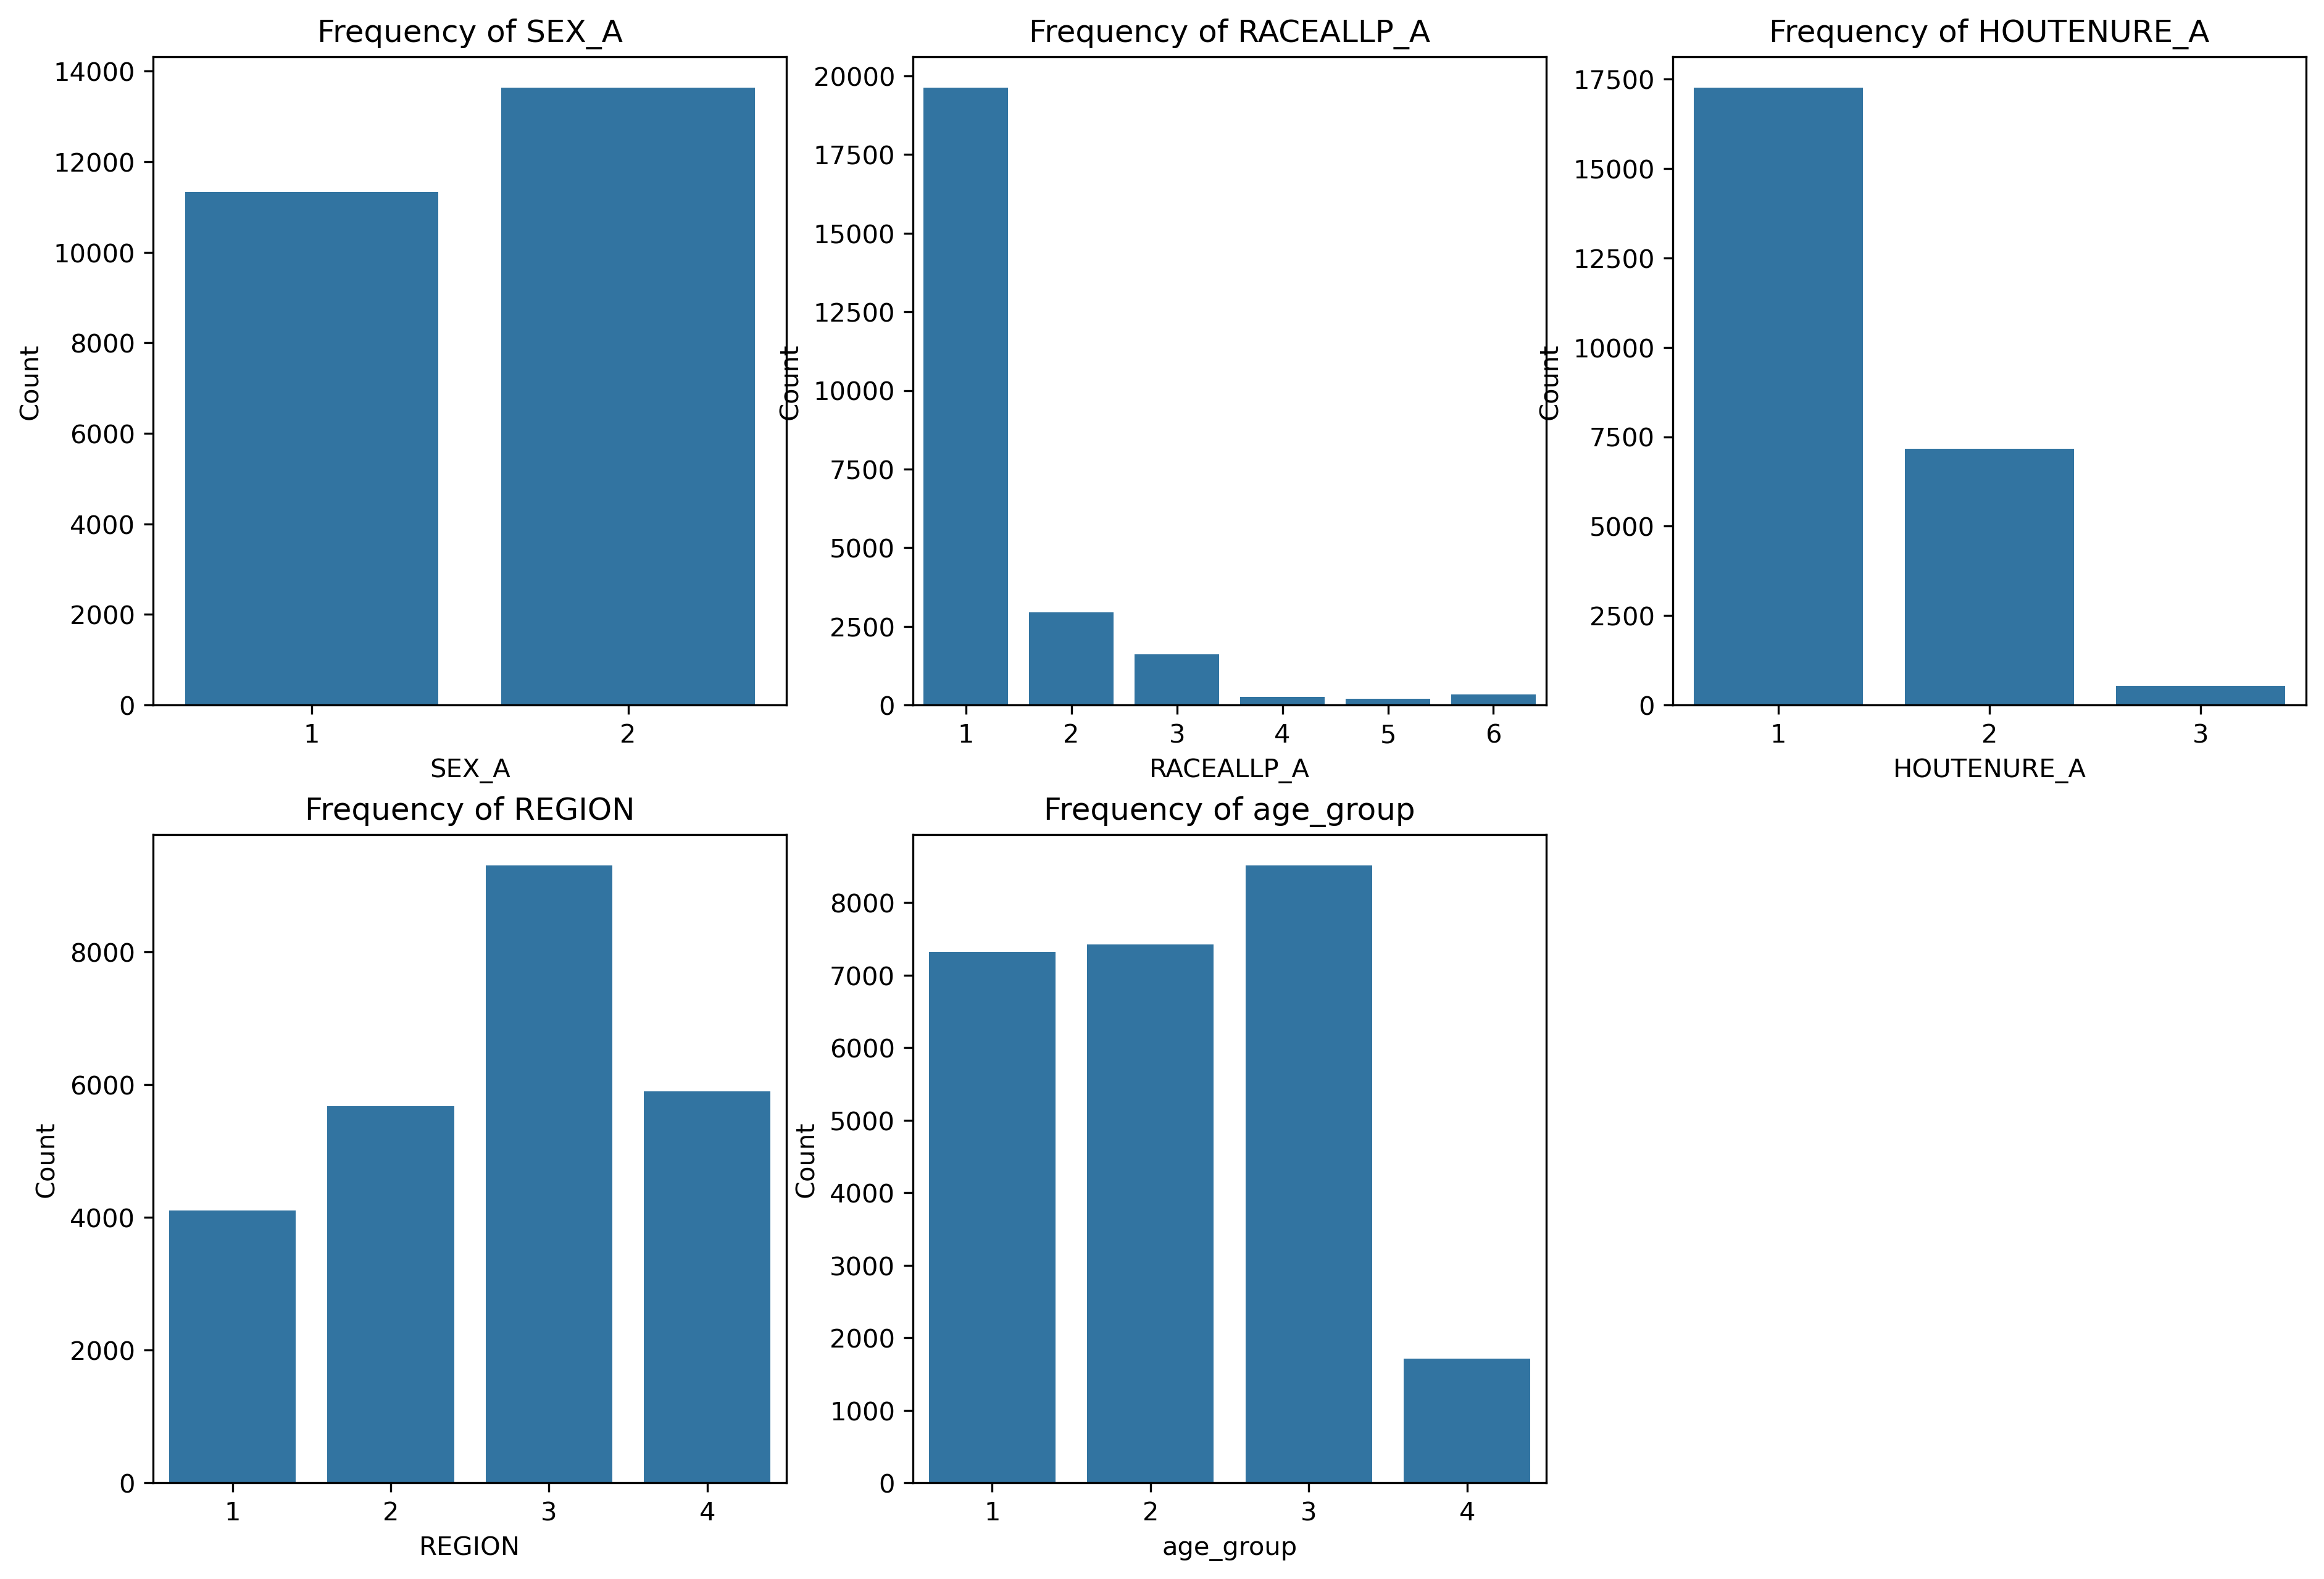
\includegraphics[width=0.9\textwidth]{../Image/singelF.png}
	\caption{Frequency of Demographic Variables}
	\label{fig:SF1}
\end{figure}
\begin{figure}[!h]
	\centering
	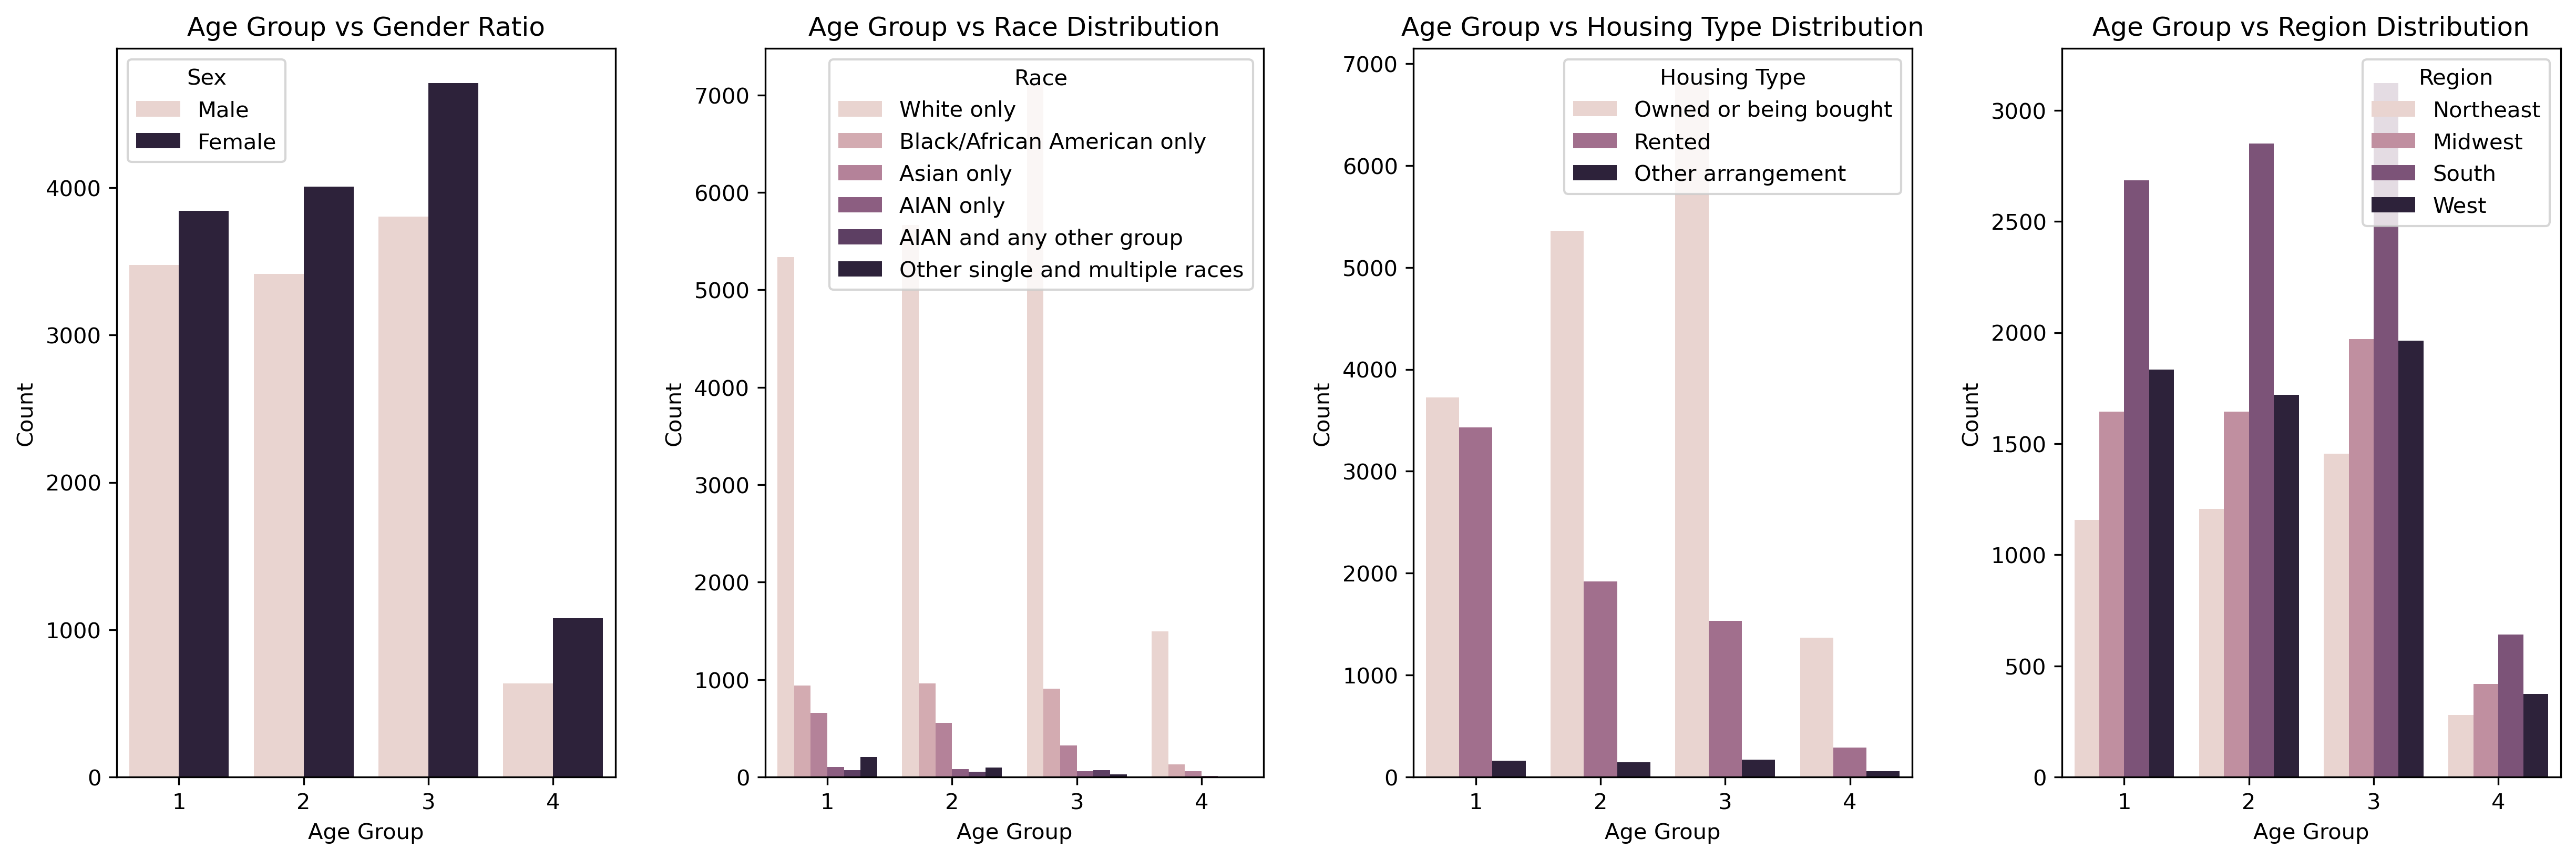
\includegraphics[width=0.9\textwidth]{../Image/age_distributions.png}
	\caption{Age Group Distributions}
	\label{fig:age_distributions}
\end{figure}

\begin{figure}[!h]
	\centering
	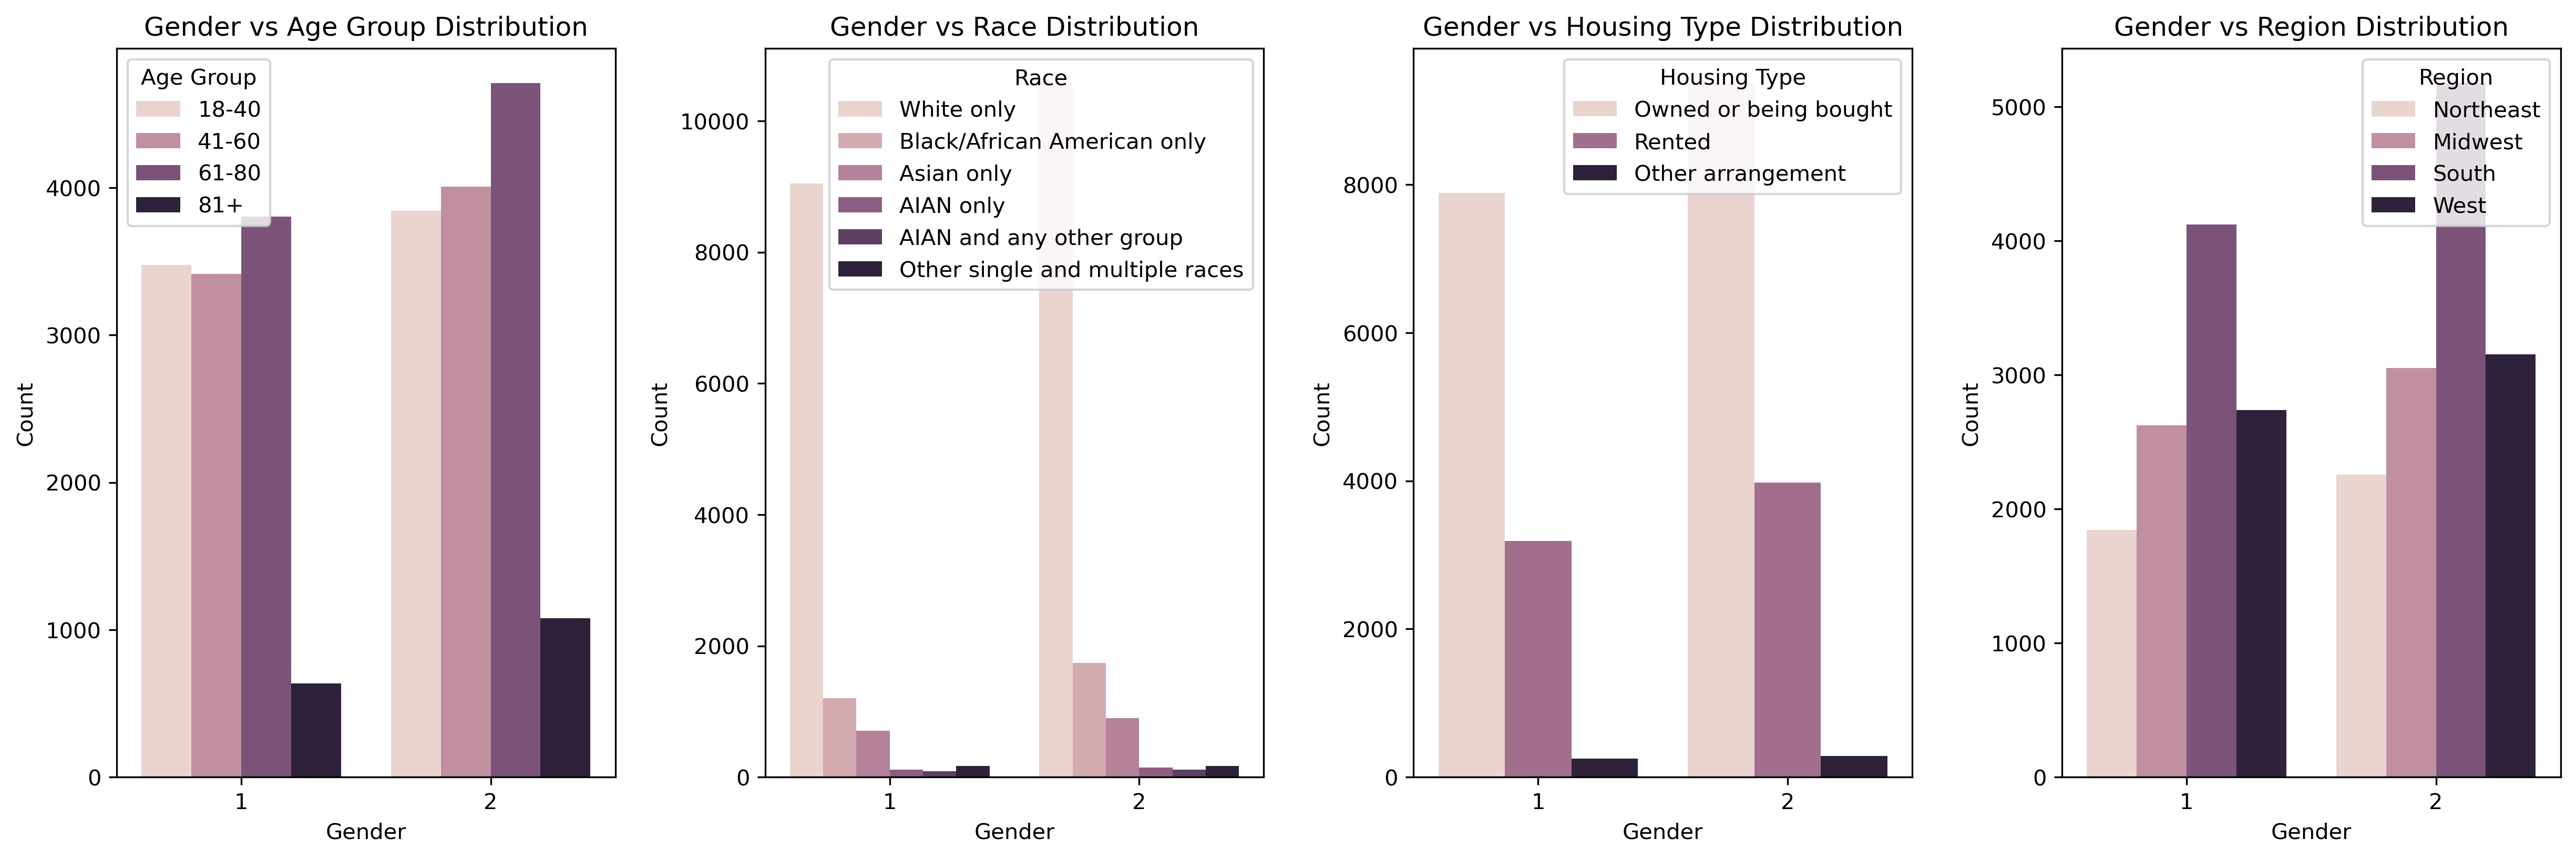
\includegraphics[width=0.9\textwidth]{../Image/sex_distributions.png}
	\caption{Sex Distributions}
	\label{fig:sex_distributions}
\end{figure}
\newpage
\begin{figure}[!h]
	\centering
	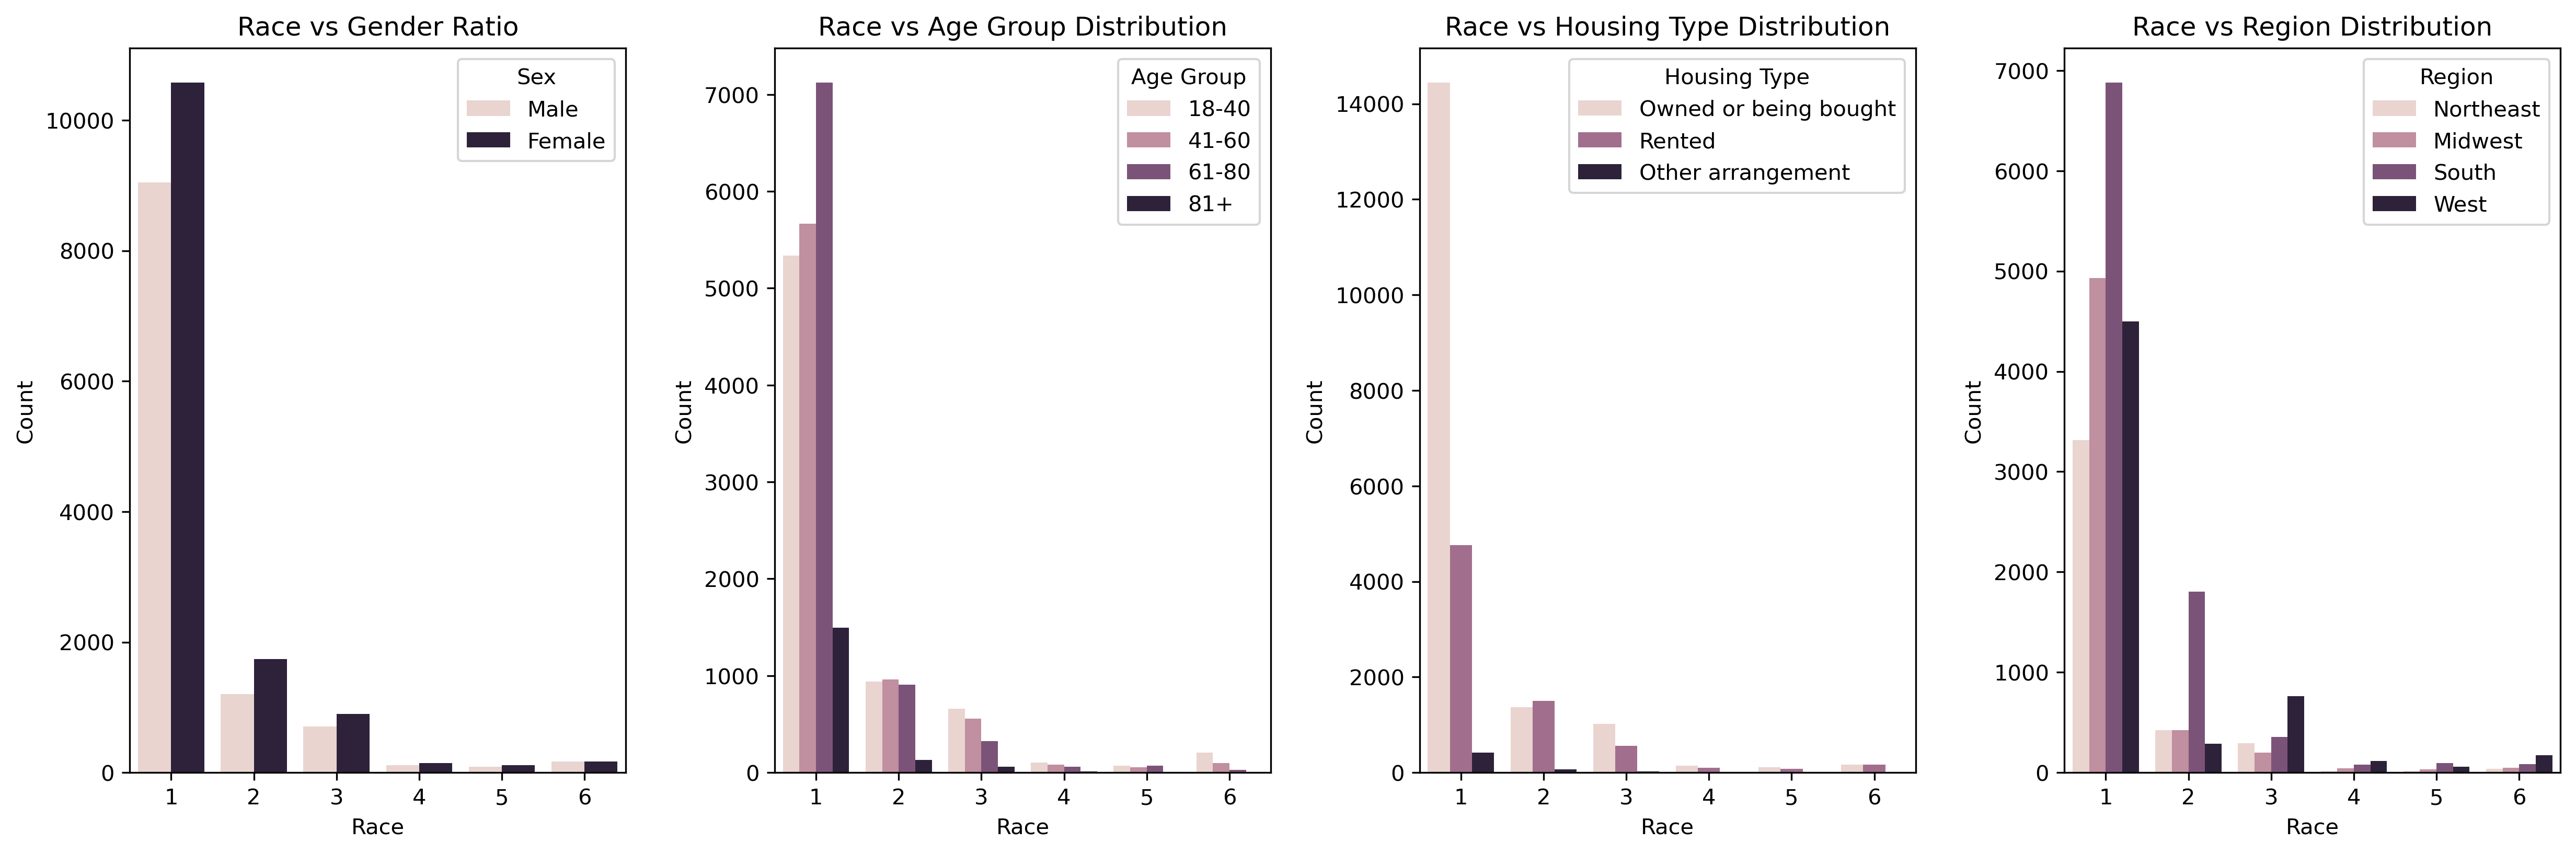
\includegraphics[width=0.9\textwidth]{../Image/race_distributions.png}
	\caption{Race Distributions}
	\label{fig:race_distributions}
\end{figure}
\begin{figure}[!h]
	\centering
	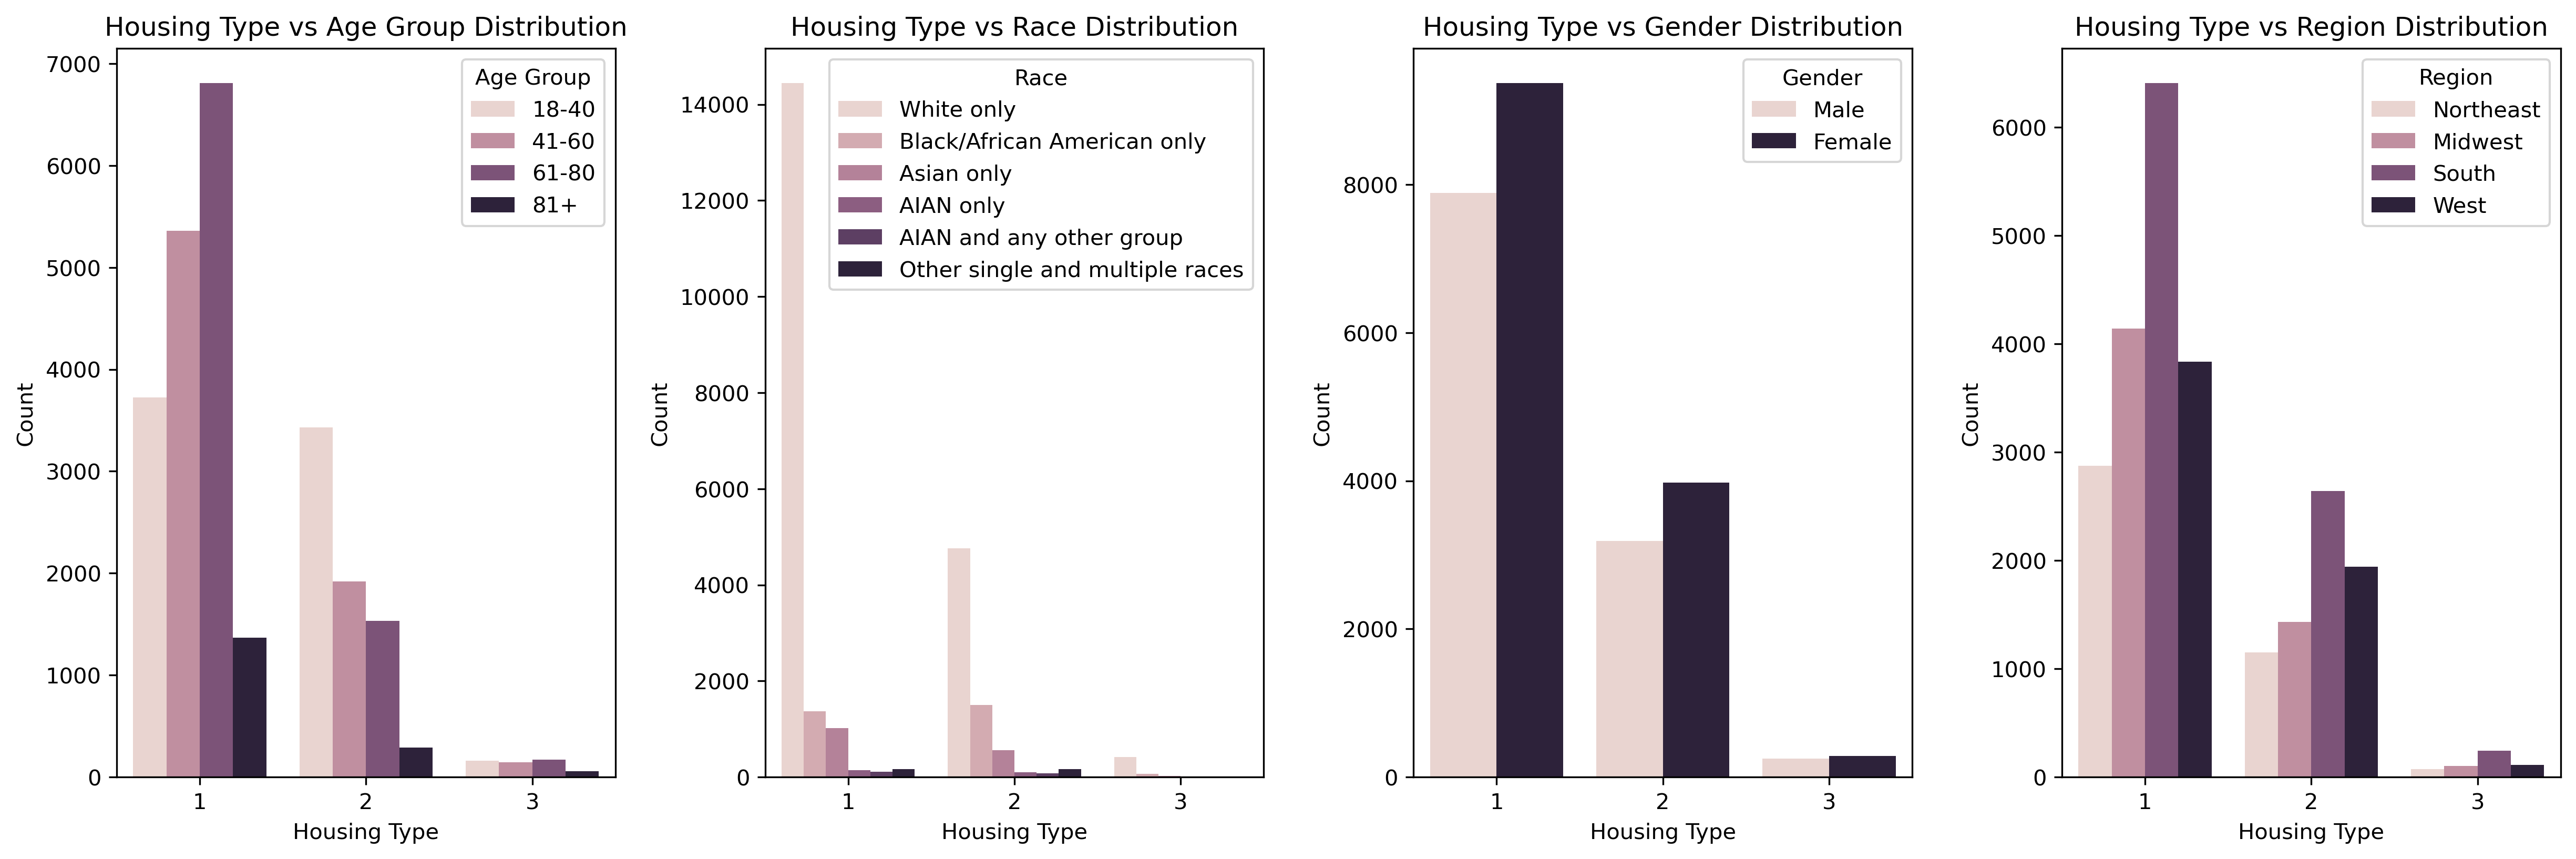
\includegraphics[width=0.9\textwidth]{../Image/house_distributions.png}
	\caption{Residential Distributions}
	\label{fig:house_distributions}
\end{figure}
\begin{figure}[!h]
	\centering
	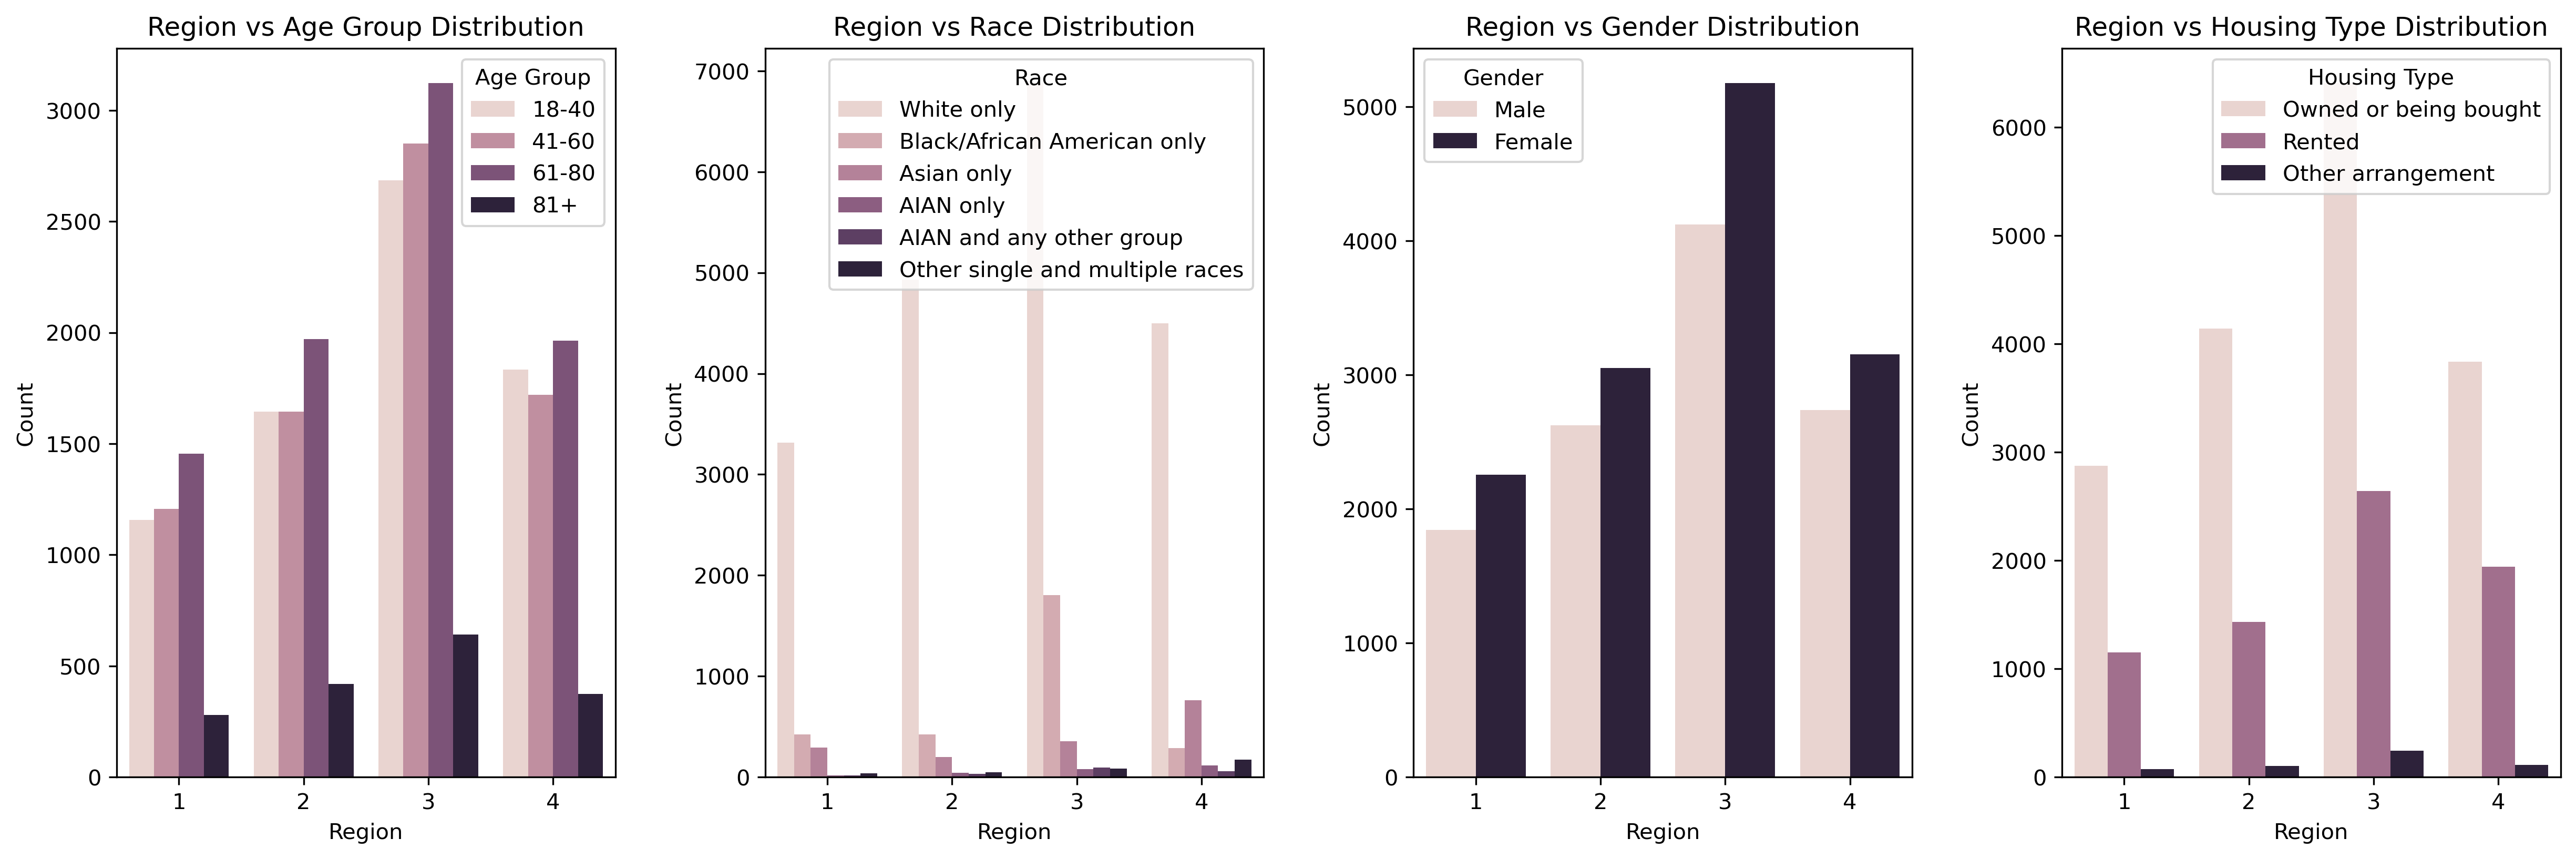
\includegraphics[width=0.9\textwidth]{../Image/region_distributions.png}
	\caption{Region Distributions}
	\label{fig:region_distributions}
\end{figure}

Through these bar charts, we can identify a few issues that may have implications for our subsequent analysis. There is a huge disparity in the number of people counted by race in our dataset, with “white only” far outnumbering any of the other races, even more than they do combined. In terms of residence, there are also significantly more people living in the “west” than anywhere else. In terms of age groups, divided into groups of nearly 20 years old, it can be seen that the number of people over 80 years old is significantly lower than that of any other group. These strengths and weaknesses are reflected in the data, and will be reflected in the habits of life. And lifestyle habits are just as important as a driver of the emergence of these data. The same holds true for cardiovascular diseases. So we can't ignore statistically weak data groups.

First, racial differences may mean that we have a statistical bias in studying certain health issues. For example, certain diseases may be more prevalent in certain races, so an uneven racial distribution may affect the accuracy of results when conducting epidemiologic studies.

Second, differences in geographic location may also have a significant impact on health outcomes. Populations in different regions may have different lifestyles, diets, and healthcare resources, all of which may affect the incidence and diagnosis of cardiovascular diseases. Thus, having significantly more people living in the “west” than in other areas may bias the analysis of the overall data.

Finally, differences in age subgroups are also noteworthy. Age is an important risk factor for cardiovascular disease, and the low proportion of people over the age of 80 may have resulted in an inadequate sample to analyze the health status of the older age groups, which may affect the reliability of our conclusions.

Our conclusions based on this data will still largely receive the influence of these data biases. In this report, I would mostly compare the data of the survey respondents in the same group, such as how many white people have a probability of having a stroke or how many white men have a probability of having a stroke. However, after adding multiple qualifications, the sample size of available studies was low and their findings were not generalizable.

In the future in order to analyze the data more accurately, we may need more and more detailed data in order to weight these variables. In this way, we can minimize the impact of data bias on the results, leading to more reliable findings. These differences and biases need to be carefully considered in the analysis to ensure that our results are scientific and fair to any group.

\newpage
\section{Task 2}
\subsection{Life Styles with Demographics}
In order to explore the relationship between demographic and life styles, I selected several dietary habits, such as the frequency of drinking pure fruit juice and the frequency of eating vegetables, as research references. The table showing below presents the diet of different groups.

\begin{table}[!h]
	\centering
	\scalebox{0.3}{
	\begin{tabular}{lllllllllllllllllllllllllllll}
		\cline{1-29}
		\multicolumn{1}{c}{} &
		\multicolumn{4}{|c}{Number of times drank pure fruit juice} &
		\multicolumn{4}{c}{Number of times drank coffee or tea with sugar} &
		\multicolumn{4}{c}{Number of times eat salad} &
		\multicolumn{4}{c}{Number of times eat fried potatoes} &
		\multicolumn{4}{c}{Number of times eat beans} &
		\multicolumn{4}{c}{Number of times eat pizza} &
		\multicolumn{4}{c}{Number of times eat other vegetables} \\
		\multicolumn{1}{c}{} &
		\multicolumn{1}{|r}{Never} &
		\multicolumn{1}{r}{Daily} &
		\multicolumn{1}{r}{Weekly} &
		\multicolumn{1}{r}{Monthly} &
		\multicolumn{1}{r}{Never} &
		\multicolumn{1}{r}{Daily} &
		\multicolumn{1}{r}{Weekly} &
		\multicolumn{1}{r}{Monthly} &
		\multicolumn{1}{r}{Never} &
		\multicolumn{1}{r}{Daily} &
		\multicolumn{1}{r}{Weekly} &
		\multicolumn{1}{r}{Monthly} &
		\multicolumn{1}{r}{Never} &
		\multicolumn{1}{r}{Daily} &
		\multicolumn{1}{r}{Weekly} &
		\multicolumn{1}{r}{Monthly} &
		\multicolumn{1}{r}{Never} &
		\multicolumn{1}{r}{Daily} &
		\multicolumn{1}{r}{Weekly} &
		\multicolumn{1}{r}{Monthly} &
		\multicolumn{1}{r}{Never} &
		\multicolumn{1}{r}{Daily} &
		\multicolumn{1}{r}{Weekly} &
		\multicolumn{1}{r}{Monthly} &
		\multicolumn{1}{r}{Never} &
		\multicolumn{1}{r}{Daily} &
		\multicolumn{1}{r}{Weekly} &
		\multicolumn{1}{r}{Monthly} \\
		\cline{1-29}
		\multicolumn{1}{r}{AGE} &
		\multicolumn{1}{|r}{} &
		\multicolumn{1}{r}{} &
		\multicolumn{1}{r}{} &
		\multicolumn{1}{r}{} &
		\multicolumn{1}{r}{} &
		\multicolumn{1}{r}{} &
		\multicolumn{1}{r}{} &
		\multicolumn{1}{r}{} &
		\multicolumn{1}{r}{} &
		\multicolumn{1}{r}{} &
		\multicolumn{1}{r}{} &
		\multicolumn{1}{r}{} &
		\multicolumn{1}{r}{} &
		\multicolumn{1}{r}{} &
		\multicolumn{1}{r}{} &
		\multicolumn{1}{r}{} &
		\multicolumn{1}{r}{} &
		\multicolumn{1}{r}{} &
		\multicolumn{1}{r}{} &
		\multicolumn{1}{r}{} &
		\multicolumn{1}{r}{} &
		\multicolumn{1}{r}{} &
		\multicolumn{1}{r}{} &
		\multicolumn{1}{r}{} &
		\multicolumn{1}{r}{} &
		\multicolumn{1}{r}{} &
		\multicolumn{1}{r}{} &
		\multicolumn{1}{r}{} \\
		\multicolumn{1}{r}{18-40\hspace{1em}} &
		\multicolumn{1}{|r}{2,879} &
		\multicolumn{1}{r}{730} &
		\multicolumn{1}{r}{1,799} &
		\multicolumn{1}{r}{1,832} &
		\multicolumn{1}{r}{2,986} &
		\multicolumn{1}{r}{1,842} &
		\multicolumn{1}{r}{1,371} &
		\multicolumn{1}{r}{1,041} &
		\multicolumn{1}{r}{836} &
		\multicolumn{1}{r}{1,114} &
		\multicolumn{1}{r}{3,698} &
		\multicolumn{1}{r}{1,592} &
		\multicolumn{1}{r}{799} &
		\multicolumn{1}{r}{225} &
		\multicolumn{1}{r}{3,543} &
		\multicolumn{1}{r}{2,673} &
		\multicolumn{1}{r}{2,046} &
		\multicolumn{1}{r}{205} &
		\multicolumn{1}{r}{2,345} &
		\multicolumn{1}{r}{2,644} &
		\multicolumn{1}{r}{754} &
		\multicolumn{1}{r}{54} &
		\multicolumn{1}{r}{2,114} &
		\multicolumn{1}{r}{4,318} &
		\multicolumn{1}{r}{306} &
		\multicolumn{1}{r}{2,668} &
		\multicolumn{1}{r}{3,063} &
		\multicolumn{1}{r}{1,203} \\
		\multicolumn{1}{r}{} &
		\multicolumn{1}{|r}{(39.77\%)} &
		\multicolumn{1}{r}{(10.08\%)} &
		\multicolumn{1}{r}{(24.85\%)} &
		\multicolumn{1}{r}{(25.30\%)} &
		\multicolumn{1}{r}{(41.24\%)} &
		\multicolumn{1}{r}{(25.44\%)} &
		\multicolumn{1}{r}{(18.94\%)} &
		\multicolumn{1}{r}{(14.38\%)} &
		\multicolumn{1}{r}{(11.55\%)} &
		\multicolumn{1}{r}{(15.39\%)} &
		\multicolumn{1}{r}{(51.08\%)} &
		\multicolumn{1}{r}{(21.99\%)} &
		\multicolumn{1}{r}{(11.04\%)} &
		\multicolumn{1}{r}{(3.11\%)} &
		\multicolumn{1}{r}{(48.94\%)} &
		\multicolumn{1}{r}{(36.92\%)} &
		\multicolumn{1}{r}{(28.26\%)} &
		\multicolumn{1}{r}{(2.83\%)} &
		\multicolumn{1}{r}{(32.39\%)} &
		\multicolumn{1}{r}{(36.52\%)} &
		\multicolumn{1}{r}{(10.41\%)} &
		\multicolumn{1}{r}{(0.75\%)} &
		\multicolumn{1}{r}{(29.20\%)} &
		\multicolumn{1}{r}{(59.64\%)} &
		\multicolumn{1}{r}{(4.23\%)} &
		\multicolumn{1}{r}{(36.85\%)} &
		\multicolumn{1}{r}{(42.31\%)} &
		\multicolumn{1}{r}{(16.62\%)} \\
		\multicolumn{1}{r}{} &
		\multicolumn{1}{|r}{} &
		\multicolumn{1}{r}{} &
		\multicolumn{1}{r}{} &
		\multicolumn{1}{r}{} &
		\multicolumn{1}{r}{} &
		\multicolumn{1}{r}{} &
		\multicolumn{1}{r}{} &
		\multicolumn{1}{r}{} &
		\multicolumn{1}{r}{} &
		\multicolumn{1}{r}{} &
		\multicolumn{1}{r}{} &
		\multicolumn{1}{r}{} &
		\multicolumn{1}{r}{} &
		\multicolumn{1}{r}{} &
		\multicolumn{1}{r}{} &
		\multicolumn{1}{r}{} &
		\multicolumn{1}{r}{} &
		\multicolumn{1}{r}{} &
		\multicolumn{1}{r}{} &
		\multicolumn{1}{r}{} &
		\multicolumn{1}{r}{} &
		\multicolumn{1}{r}{} &
		\multicolumn{1}{r}{} &
		\multicolumn{1}{r}{} &
		\multicolumn{1}{r}{} &
		\multicolumn{1}{r}{} &
		\multicolumn{1}{r}{} &
		\multicolumn{1}{r}{} \\
		\multicolumn{1}{r}{41-60\hspace{1em}} &
		\multicolumn{1}{|r}{3,601} &
		\multicolumn{1}{r}{733} &
		\multicolumn{1}{r}{1,463} &
		\multicolumn{1}{r}{1,564} &
		\multicolumn{1}{r}{3,491} &
		\multicolumn{1}{r}{2,148} &
		\multicolumn{1}{r}{1,006} &
		\multicolumn{1}{r}{716} &
		\multicolumn{1}{r}{664} &
		\multicolumn{1}{r}{1,315} &
		\multicolumn{1}{r}{3,822} &
		\multicolumn{1}{r}{1,560} &
		\multicolumn{1}{r}{1,447} &
		\multicolumn{1}{r}{174} &
		\multicolumn{1}{r}{2,786} &
		\multicolumn{1}{r}{2,954} &
		\multicolumn{1}{r}{1,823} &
		\multicolumn{1}{r}{209} &
		\multicolumn{1}{r}{2,465} &
		\multicolumn{1}{r}{2,864} &
		\multicolumn{1}{r}{1,172} &
		\multicolumn{1}{r}{55} &
		\multicolumn{1}{r}{1,754} &
		\multicolumn{1}{r}{4,380} &
		\multicolumn{1}{r}{312} &
		\multicolumn{1}{r}{2,762} &
		\multicolumn{1}{r}{3,097} &
		\multicolumn{1}{r}{1,190} \\
		\multicolumn{1}{r}{} &
		\multicolumn{1}{|r}{(48.92\%)} &
		\multicolumn{1}{r}{(9.96\%)} &
		\multicolumn{1}{r}{(19.88\%)} &
		\multicolumn{1}{r}{(21.25\%)} &
		\multicolumn{1}{r}{(47.43\%)} &
		\multicolumn{1}{r}{(29.18\%)} &
		\multicolumn{1}{r}{(13.67\%)} &
		\multicolumn{1}{r}{(9.73\%)} &
		\multicolumn{1}{r}{(9.02\%)} &
		\multicolumn{1}{r}{(17.86\%)} &
		\multicolumn{1}{r}{(51.92\%)} &
		\multicolumn{1}{r}{(21.19\%)} &
		\multicolumn{1}{r}{(19.66\%)} &
		\multicolumn{1}{r}{(2.36\%)} &
		\multicolumn{1}{r}{(37.85\%)} &
		\multicolumn{1}{r}{(40.13\%)} &
		\multicolumn{1}{r}{(24.77\%)} &
		\multicolumn{1}{r}{(2.84\%)} &
		\multicolumn{1}{r}{(33.49\%)} &
		\multicolumn{1}{r}{(38.91\%)} &
		\multicolumn{1}{r}{(15.92\%)} &
		\multicolumn{1}{r}{(0.75\%)} &
		\multicolumn{1}{r}{(23.83\%)} &
		\multicolumn{1}{r}{(59.50\%)} &
		\multicolumn{1}{r}{(4.24\%)} &
		\multicolumn{1}{r}{(37.52\%)} &
		\multicolumn{1}{r}{(42.07\%)} &
		\multicolumn{1}{r}{(16.17\%)} \\
		\multicolumn{1}{r}{} &
		\multicolumn{1}{|r}{} &
		\multicolumn{1}{r}{} &
		\multicolumn{1}{r}{} &
		\multicolumn{1}{r}{} &
		\multicolumn{1}{r}{} &
		\multicolumn{1}{r}{} &
		\multicolumn{1}{r}{} &
		\multicolumn{1}{r}{} &
		\multicolumn{1}{r}{} &
		\multicolumn{1}{r}{} &
		\multicolumn{1}{r}{} &
		\multicolumn{1}{r}{} &
		\multicolumn{1}{r}{} &
		\multicolumn{1}{r}{} &
		\multicolumn{1}{r}{} &
		\multicolumn{1}{r}{} &
		\multicolumn{1}{r}{} &
		\multicolumn{1}{r}{} &
		\multicolumn{1}{r}{} &
		\multicolumn{1}{r}{} &
		\multicolumn{1}{r}{} &
		\multicolumn{1}{r}{} &
		\multicolumn{1}{r}{} &
		\multicolumn{1}{r}{} &
		\multicolumn{1}{r}{} &
		\multicolumn{1}{r}{} &
		\multicolumn{1}{r}{} &
		\multicolumn{1}{r}{} \\
		\multicolumn{1}{r}{61-80\hspace{1em}} &
		\multicolumn{1}{|r}{4,232} &
		\multicolumn{1}{r}{1,113} &
		\multicolumn{1}{r}{1,570} &
		\multicolumn{1}{r}{1,519} &
		\multicolumn{1}{r}{4,693} &
		\multicolumn{1}{r}{2,276} &
		\multicolumn{1}{r}{848} &
		\multicolumn{1}{r}{617} &
		\multicolumn{1}{r}{832} &
		\multicolumn{1}{r}{1,542} &
		\multicolumn{1}{r}{4,322} &
		\multicolumn{1}{r}{1,738} &
		\multicolumn{1}{r}{2,235} &
		\multicolumn{1}{r}{128} &
		\multicolumn{1}{r}{2,657} &
		\multicolumn{1}{r}{3,414} &
		\multicolumn{1}{r}{2,029} &
		\multicolumn{1}{r}{206} &
		\multicolumn{1}{r}{2,686} &
		\multicolumn{1}{r}{3,513} &
		\multicolumn{1}{r}{2,005} &
		\multicolumn{1}{r}{36} &
		\multicolumn{1}{r}{1,281} &
		\multicolumn{1}{r}{5,112} &
		\multicolumn{1}{r}{350} &
		\multicolumn{1}{r}{3,196} &
		\multicolumn{1}{r}{3,422} &
		\multicolumn{1}{r}{1,466} \\
		\multicolumn{1}{r}{} &
		\multicolumn{1}{|r}{(50.18\%)} &
		\multicolumn{1}{r}{(13.20\%)} &
		\multicolumn{1}{r}{(18.62\%)} &
		\multicolumn{1}{r}{(18.01\%)} &
		\multicolumn{1}{r}{(55.64\%)} &
		\multicolumn{1}{r}{(26.99\%)} &
		\multicolumn{1}{r}{(10.05\%)} &
		\multicolumn{1}{r}{(7.32\%)} &
		\multicolumn{1}{r}{(9.86\%)} &
		\multicolumn{1}{r}{(18.28\%)} &
		\multicolumn{1}{r}{(51.24\%)} &
		\multicolumn{1}{r}{(20.61\%)} &
		\multicolumn{1}{r}{(26.50\%)} &
		\multicolumn{1}{r}{(1.52\%)} &
		\multicolumn{1}{r}{(31.50\%)} &
		\multicolumn{1}{r}{(40.48\%)} &
		\multicolumn{1}{r}{(24.06\%)} &
		\multicolumn{1}{r}{(2.44\%)} &
		\multicolumn{1}{r}{(31.85\%)} &
		\multicolumn{1}{r}{(41.65\%)} &
		\multicolumn{1}{r}{(23.77\%)} &
		\multicolumn{1}{r}{(0.43\%)} &
		\multicolumn{1}{r}{(15.19\%)} &
		\multicolumn{1}{r}{(60.61\%)} &
		\multicolumn{1}{r}{(4.15\%)} &
		\multicolumn{1}{r}{(37.89\%)} &
		\multicolumn{1}{r}{(40.57\%)} &
		\multicolumn{1}{r}{(17.38\%)} \\
		\multicolumn{1}{r}{} &
		\multicolumn{1}{|r}{} &
		\multicolumn{1}{r}{} &
		\multicolumn{1}{r}{} &
		\multicolumn{1}{r}{} &
		\multicolumn{1}{r}{} &
		\multicolumn{1}{r}{} &
		\multicolumn{1}{r}{} &
		\multicolumn{1}{r}{} &
		\multicolumn{1}{r}{} &
		\multicolumn{1}{r}{} &
		\multicolumn{1}{r}{} &
		\multicolumn{1}{r}{} &
		\multicolumn{1}{r}{} &
		\multicolumn{1}{r}{} &
		\multicolumn{1}{r}{} &
		\multicolumn{1}{r}{} &
		\multicolumn{1}{r}{} &
		\multicolumn{1}{r}{} &
		\multicolumn{1}{r}{} &
		\multicolumn{1}{r}{} &
		\multicolumn{1}{r}{} &
		\multicolumn{1}{r}{} &
		\multicolumn{1}{r}{} &
		\multicolumn{1}{r}{} &
		\multicolumn{1}{r}{} &
		\multicolumn{1}{r}{} &
		\multicolumn{1}{r}{} &
		\multicolumn{1}{r}{} \\
		\multicolumn{1}{r}{81+\hspace{1em}} &
		\multicolumn{1}{|r}{700} &
		\multicolumn{1}{r}{407} &
		\multicolumn{1}{r}{321} &
		\multicolumn{1}{r}{240} &
		\multicolumn{1}{r}{981} &
		\multicolumn{1}{r}{471} &
		\multicolumn{1}{r}{135} &
		\multicolumn{1}{r}{81} &
		\multicolumn{1}{r}{255} &
		\multicolumn{1}{r}{352} &
		\multicolumn{1}{r}{771} &
		\multicolumn{1}{r}{290} &
		\multicolumn{1}{r}{508} &
		\multicolumn{1}{r}{32} &
		\multicolumn{1}{r}{539} &
		\multicolumn{1}{r}{589} &
		\multicolumn{1}{r}{393} &
		\multicolumn{1}{r}{49} &
		\multicolumn{1}{r}{574} &
		\multicolumn{1}{r}{652} &
		\multicolumn{1}{r}{528} &
		\multicolumn{1}{r}{14} &
		\multicolumn{1}{r}{198} &
		\multicolumn{1}{r}{928} &
		\multicolumn{1}{r}{65} &
		\multicolumn{1}{r}{709} &
		\multicolumn{1}{r}{681} &
		\multicolumn{1}{r}{213} \\
		\multicolumn{1}{r}{} &
		\multicolumn{1}{|r}{(41.97\%)} &
		\multicolumn{1}{r}{(24.40\%)} &
		\multicolumn{1}{r}{(19.24\%)} &
		\multicolumn{1}{r}{(14.39\%)} &
		\multicolumn{1}{r}{(58.81\%)} &
		\multicolumn{1}{r}{(28.24\%)} &
		\multicolumn{1}{r}{(8.09\%)} &
		\multicolumn{1}{r}{(4.86\%)} &
		\multicolumn{1}{r}{(15.29\%)} &
		\multicolumn{1}{r}{(21.10\%)} &
		\multicolumn{1}{r}{(46.22\%)} &
		\multicolumn{1}{r}{(17.39\%)} &
		\multicolumn{1}{r}{(30.46\%)} &
		\multicolumn{1}{r}{(1.92\%)} &
		\multicolumn{1}{r}{(32.31\%)} &
		\multicolumn{1}{r}{(35.31\%)} &
		\multicolumn{1}{r}{(23.56\%)} &
		\multicolumn{1}{r}{(2.94\%)} &
		\multicolumn{1}{r}{(34.41\%)} &
		\multicolumn{1}{r}{(39.09\%)} &
		\multicolumn{1}{r}{(31.65\%)} &
		\multicolumn{1}{r}{(0.84\%)} &
		\multicolumn{1}{r}{(11.87\%)} &
		\multicolumn{1}{r}{(55.64\%)} &
		\multicolumn{1}{r}{(3.90\%)} &
		\multicolumn{1}{r}{(42.51\%)} &
		\multicolumn{1}{r}{(40.83\%)} &
		\multicolumn{1}{r}{(12.77\%)} \\
		\multicolumn{1}{r}{} &
		\multicolumn{1}{|r}{} &
		\multicolumn{1}{r}{} &
		\multicolumn{1}{r}{} &
		\multicolumn{1}{r}{} &
		\multicolumn{1}{r}{} &
		\multicolumn{1}{r}{} &
		\multicolumn{1}{r}{} &
		\multicolumn{1}{r}{} &
		\multicolumn{1}{r}{} &
		\multicolumn{1}{r}{} &
		\multicolumn{1}{r}{} &
		\multicolumn{1}{r}{} &
		\multicolumn{1}{r}{} &
		\multicolumn{1}{r}{} &
		\multicolumn{1}{r}{} &
		\multicolumn{1}{r}{} &
		\multicolumn{1}{r}{} &
		\multicolumn{1}{r}{} &
		\multicolumn{1}{r}{} &
		\multicolumn{1}{r}{} &
		\multicolumn{1}{r}{} &
		\multicolumn{1}{r}{} &
		\multicolumn{1}{r}{} &
		\multicolumn{1}{r}{} &
		\multicolumn{1}{r}{} &
		\multicolumn{1}{r}{} &
		\multicolumn{1}{r}{} &
		\multicolumn{1}{r}{} \\
		\multicolumn{1}{r}{SEX} &
		\multicolumn{1}{|r}{} &
		\multicolumn{1}{r}{} &
		\multicolumn{1}{r}{} &
		\multicolumn{1}{r}{} &
		\multicolumn{1}{r}{} &
		\multicolumn{1}{r}{} &
		\multicolumn{1}{r}{} &
		\multicolumn{1}{r}{} &
		\multicolumn{1}{r}{} &
		\multicolumn{1}{r}{} &
		\multicolumn{1}{r}{} &
		\multicolumn{1}{r}{} &
		\multicolumn{1}{r}{} &
		\multicolumn{1}{r}{} &
		\multicolumn{1}{r}{} &
		\multicolumn{1}{r}{} &
		\multicolumn{1}{r}{} &
		\multicolumn{1}{r}{} &
		\multicolumn{1}{r}{} &
		\multicolumn{1}{r}{} &
		\multicolumn{1}{r}{} &
		\multicolumn{1}{r}{} &
		\multicolumn{1}{r}{} &
		\multicolumn{1}{r}{} &
		\multicolumn{1}{r}{} &
		\multicolumn{1}{r}{} &
		\multicolumn{1}{r}{} &
		\multicolumn{1}{r}{} \\
		\multicolumn{1}{r}{Male\hspace{1em}} &
		\multicolumn{1}{|r}{4,649} &
		\multicolumn{1}{r}{1,543} &
		\multicolumn{1}{r}{2,605} &
		\multicolumn{1}{r}{2,407} &
		\multicolumn{1}{r}{5,810} &
		\multicolumn{1}{r}{2,839} &
		\multicolumn{1}{r}{1,500} &
		\multicolumn{1}{r}{1,055} &
		\multicolumn{1}{r}{1,461} &
		\multicolumn{1}{r}{1,646} &
		\multicolumn{1}{r}{5,633} &
		\multicolumn{1}{r}{2,464} &
		\multicolumn{1}{r}{1,881} &
		\multicolumn{1}{r}{310} &
		\multicolumn{1}{r}{4,917} &
		\multicolumn{1}{r}{4,096} &
		\multicolumn{1}{r}{2,652} &
		\multicolumn{1}{r}{310} &
		\multicolumn{1}{r}{3,924} &
		\multicolumn{1}{r}{4,318} &
		\multicolumn{1}{r}{1,766} &
		\multicolumn{1}{r}{85} &
		\multicolumn{1}{r}{2,804} &
		\multicolumn{1}{r}{6,549} &
		\multicolumn{1}{r}{606} &
		\multicolumn{1}{r}{3,616} &
		\multicolumn{1}{r}{4,990} &
		\multicolumn{1}{r}{1,992} \\
		\multicolumn{1}{r}{} &
		\multicolumn{1}{|r}{(41.49\%)} &
		\multicolumn{1}{r}{(13.77\%)} &
		\multicolumn{1}{r}{(23.25\%)} &
		\multicolumn{1}{r}{(21.48\%)} &
		\multicolumn{1}{r}{(51.86\%)} &
		\multicolumn{1}{r}{(25.34\%)} &
		\multicolumn{1}{r}{(13.39\%)} &
		\multicolumn{1}{r}{(9.42\%)} &
		\multicolumn{1}{r}{(13.04\%)} &
		\multicolumn{1}{r}{(14.69\%)} &
		\multicolumn{1}{r}{(50.28\%)} &
		\multicolumn{1}{r}{(21.99\%)} &
		\multicolumn{1}{r}{(16.79\%)} &
		\multicolumn{1}{r}{(2.77\%)} &
		\multicolumn{1}{r}{(43.89\%)} &
		\multicolumn{1}{r}{(36.56\%)} &
		\multicolumn{1}{r}{(23.67\%)} &
		\multicolumn{1}{r}{(2.77\%)} &
		\multicolumn{1}{r}{(35.02\%)} &
		\multicolumn{1}{r}{(38.54\%)} &
		\multicolumn{1}{r}{(15.76\%)} &
		\multicolumn{1}{r}{(0.76\%)} &
		\multicolumn{1}{r}{(25.03\%)} &
		\multicolumn{1}{r}{(58.45\%)} &
		\multicolumn{1}{r}{(5.41\%)} &
		\multicolumn{1}{r}{(32.27\%)} &
		\multicolumn{1}{r}{(44.54\%)} &
		\multicolumn{1}{r}{(17.78\%)} \\
		\multicolumn{1}{r}{} &
		\multicolumn{1}{|r}{} &
		\multicolumn{1}{r}{} &
		\multicolumn{1}{r}{} &
		\multicolumn{1}{r}{} &
		\multicolumn{1}{r}{} &
		\multicolumn{1}{r}{} &
		\multicolumn{1}{r}{} &
		\multicolumn{1}{r}{} &
		\multicolumn{1}{r}{} &
		\multicolumn{1}{r}{} &
		\multicolumn{1}{r}{} &
		\multicolumn{1}{r}{} &
		\multicolumn{1}{r}{} &
		\multicolumn{1}{r}{} &
		\multicolumn{1}{r}{} &
		\multicolumn{1}{r}{} &
		\multicolumn{1}{r}{} &
		\multicolumn{1}{r}{} &
		\multicolumn{1}{r}{} &
		\multicolumn{1}{r}{} &
		\multicolumn{1}{r}{} &
		\multicolumn{1}{r}{} &
		\multicolumn{1}{r}{} &
		\multicolumn{1}{r}{} &
		\multicolumn{1}{r}{} &
		\multicolumn{1}{r}{} &
		\multicolumn{1}{r}{} &
		\multicolumn{1}{r}{} \\
		\multicolumn{1}{r}{Female\hspace{1em}} &
		\multicolumn{1}{|r}{6,763} &
		\multicolumn{1}{r}{1,440} &
		\multicolumn{1}{r}{2,548} &
		\multicolumn{1}{r}{2,748} &
		\multicolumn{1}{r}{6,341} &
		\multicolumn{1}{r}{3,898} &
		\multicolumn{1}{r}{1,860} &
		\multicolumn{1}{r}{1,400} &
		\multicolumn{1}{r}{1,126} &
		\multicolumn{1}{r}{2,677} &
		\multicolumn{1}{r}{6,980} &
		\multicolumn{1}{r}{2,716} &
		\multicolumn{1}{r}{3,108} &
		\multicolumn{1}{r}{249} &
		\multicolumn{1}{r}{4,608} &
		\multicolumn{1}{r}{5,534} &
		\multicolumn{1}{r}{3,639} &
		\multicolumn{1}{r}{359} &
		\multicolumn{1}{r}{4,146} &
		\multicolumn{1}{r}{5,355} &
		\multicolumn{1}{r}{2,693} &
		\multicolumn{1}{r}{74} &
		\multicolumn{1}{r}{2,543} &
		\multicolumn{1}{r}{8,189} &
		\multicolumn{1}{r}{427} &
		\multicolumn{1}{r}{5,719} &
		\multicolumn{1}{r}{5,273} &
		\multicolumn{1}{r}{2,080} \\
		\multicolumn{1}{r}{} &
		\multicolumn{1}{|r}{(50.10\%)} &
		\multicolumn{1}{r}{(10.67\%)} &
		\multicolumn{1}{r}{(18.88\%)} &
		\multicolumn{1}{r}{(20.36\%)} &
		\multicolumn{1}{r}{(46.97\%)} &
		\multicolumn{1}{r}{(28.88\%)} &
		\multicolumn{1}{r}{(13.78\%)} &
		\multicolumn{1}{r}{(10.37\%)} &
		\multicolumn{1}{r}{(8.34\%)} &
		\multicolumn{1}{r}{(19.83\%)} &
		\multicolumn{1}{r}{(51.71\%)} &
		\multicolumn{1}{r}{(20.12\%)} &
		\multicolumn{1}{r}{(23.02\%)} &
		\multicolumn{1}{r}{(1.84\%)} &
		\multicolumn{1}{r}{(34.14\%)} &
		\multicolumn{1}{r}{(41.00\%)} &
		\multicolumn{1}{r}{(26.96\%)} &
		\multicolumn{1}{r}{(2.66\%)} &
		\multicolumn{1}{r}{(30.71\%)} &
		\multicolumn{1}{r}{(39.67\%)} &
		\multicolumn{1}{r}{(19.95\%)} &
		\multicolumn{1}{r}{(0.55\%)} &
		\multicolumn{1}{r}{(18.84\%)} &
		\multicolumn{1}{r}{(60.66\%)} &
		\multicolumn{1}{r}{(3.16\%)} &
		\multicolumn{1}{r}{(42.37\%)} &
		\multicolumn{1}{r}{(39.06\%)} &
		\multicolumn{1}{r}{(15.41\%)} \\
		\multicolumn{1}{r}{} &
		\multicolumn{1}{|r}{} &
		\multicolumn{1}{r}{} &
		\multicolumn{1}{r}{} &
		\multicolumn{1}{r}{} &
		\multicolumn{1}{r}{} &
		\multicolumn{1}{r}{} &
		\multicolumn{1}{r}{} &
		\multicolumn{1}{r}{} &
		\multicolumn{1}{r}{} &
		\multicolumn{1}{r}{} &
		\multicolumn{1}{r}{} &
		\multicolumn{1}{r}{} &
		\multicolumn{1}{r}{} &
		\multicolumn{1}{r}{} &
		\multicolumn{1}{r}{} &
		\multicolumn{1}{r}{} &
		\multicolumn{1}{r}{} &
		\multicolumn{1}{r}{} &
		\multicolumn{1}{r}{} &
		\multicolumn{1}{r}{} &
		\multicolumn{1}{r}{} &
		\multicolumn{1}{r}{} &
		\multicolumn{1}{r}{} &
		\multicolumn{1}{r}{} &
		\multicolumn{1}{r}{} &
		\multicolumn{1}{r}{} &
		\multicolumn{1}{r}{} &
		\multicolumn{1}{r}{} \\
		\multicolumn{1}{r}{RACE} &
		\multicolumn{1}{|r}{} &
		\multicolumn{1}{r}{} &
		\multicolumn{1}{r}{} &
		\multicolumn{1}{r}{} &
		\multicolumn{1}{r}{} &
		\multicolumn{1}{r}{} &
		\multicolumn{1}{r}{} &
		\multicolumn{1}{r}{} &
		\multicolumn{1}{r}{} &
		\multicolumn{1}{r}{} &
		\multicolumn{1}{r}{} &
		\multicolumn{1}{r}{} &
		\multicolumn{1}{r}{} &
		\multicolumn{1}{r}{} &
		\multicolumn{1}{r}{} &
		\multicolumn{1}{r}{} &
		\multicolumn{1}{r}{} &
		\multicolumn{1}{r}{} &
		\multicolumn{1}{r}{} &
		\multicolumn{1}{r}{} &
		\multicolumn{1}{r}{} &
		\multicolumn{1}{r}{} &
		\multicolumn{1}{r}{} &
		\multicolumn{1}{r}{} &
		\multicolumn{1}{r}{} &
		\multicolumn{1}{r}{} &
		\multicolumn{1}{r}{} &
		\multicolumn{1}{r}{} \\
		\multicolumn{1}{r}{White only\hspace{1em}} &
		\multicolumn{1}{|r}{9,451} &
		\multicolumn{1}{r}{2,186} &
		\multicolumn{1}{r}{3,732} &
		\multicolumn{1}{r}{4,053} &
		\multicolumn{1}{r}{9,957} &
		\multicolumn{1}{r}{5,259} &
		\multicolumn{1}{r}{2,406} &
		\multicolumn{1}{r}{1,800} &
		\multicolumn{1}{r}{1,924} &
		\multicolumn{1}{r}{3,285} &
		\multicolumn{1}{r}{10,058} &
		\multicolumn{1}{r}{4,155} &
		\multicolumn{1}{r}{3,744} &
		\multicolumn{1}{r}{415} &
		\multicolumn{1}{r}{7,609} &
		\multicolumn{1}{r}{7,654} &
		\multicolumn{1}{r}{4,672} &
		\multicolumn{1}{r}{507} &
		\multicolumn{1}{r}{6,509} &
		\multicolumn{1}{r}{7,734} &
		\multicolumn{1}{r}{3,068} &
		\multicolumn{1}{r}{124} &
		\multicolumn{1}{r}{4,531} &
		\multicolumn{1}{r}{11,699} &
		\multicolumn{1}{r}{795} &
		\multicolumn{1}{r}{7,399} &
		\multicolumn{1}{r}{7,980} &
		\multicolumn{1}{r}{3,248} \\
		\multicolumn{1}{r}{} &
		\multicolumn{1}{|r}{(48.66\%)} &
		\multicolumn{1}{r}{(11.26\%)} &
		\multicolumn{1}{r}{(19.22\%)} &
		\multicolumn{1}{r}{(20.87\%)} &
		\multicolumn{1}{r}{(51.27\%)} &
		\multicolumn{1}{r}{(27.08\%)} &
		\multicolumn{1}{r}{(12.39\%)} &
		\multicolumn{1}{r}{(9.27\%)} &
		\multicolumn{1}{r}{(9.91\%)} &
		\multicolumn{1}{r}{(16.91\%)} &
		\multicolumn{1}{r}{(51.79\%)} &
		\multicolumn{1}{r}{(21.39\%)} &
		\multicolumn{1}{r}{(19.28\%)} &
		\multicolumn{1}{r}{(2.14\%)} &
		\multicolumn{1}{r}{(39.18\%)} &
		\multicolumn{1}{r}{(39.41\%)} &
		\multicolumn{1}{r}{(24.06\%)} &
		\multicolumn{1}{r}{(2.61\%)} &
		\multicolumn{1}{r}{(33.51\%)} &
		\multicolumn{1}{r}{(39.82\%)} &
		\multicolumn{1}{r}{(15.80\%)} &
		\multicolumn{1}{r}{(0.64\%)} &
		\multicolumn{1}{r}{(23.33\%)} &
		\multicolumn{1}{r}{(60.24\%)} &
		\multicolumn{1}{r}{(4.09\%)} &
		\multicolumn{1}{r}{(38.10\%)} &
		\multicolumn{1}{r}{(41.09\%)} &
		\multicolumn{1}{r}{(16.72\%)} \\
		\multicolumn{1}{r}{} &
		\multicolumn{1}{|r}{} &
		\multicolumn{1}{r}{} &
		\multicolumn{1}{r}{} &
		\multicolumn{1}{r}{} &
		\multicolumn{1}{r}{} &
		\multicolumn{1}{r}{} &
		\multicolumn{1}{r}{} &
		\multicolumn{1}{r}{} &
		\multicolumn{1}{r}{} &
		\multicolumn{1}{r}{} &
		\multicolumn{1}{r}{} &
		\multicolumn{1}{r}{} &
		\multicolumn{1}{r}{} &
		\multicolumn{1}{r}{} &
		\multicolumn{1}{r}{} &
		\multicolumn{1}{r}{} &
		\multicolumn{1}{r}{} &
		\multicolumn{1}{r}{} &
		\multicolumn{1}{r}{} &
		\multicolumn{1}{r}{} &
		\multicolumn{1}{r}{} &
		\multicolumn{1}{r}{} &
		\multicolumn{1}{r}{} &
		\multicolumn{1}{r}{} &
		\multicolumn{1}{r}{} &
		\multicolumn{1}{r}{} &
		\multicolumn{1}{r}{} &
		\multicolumn{1}{r}{} \\
		\multicolumn{1}{r}{Black/African American only\hspace{1em}} &
		\multicolumn{1}{|r}{896} &
		\multicolumn{1}{r}{563} &
		\multicolumn{1}{r}{857} &
		\multicolumn{1}{r}{587} &
		\multicolumn{1}{r}{1,148} &
		\multicolumn{1}{r}{769} &
		\multicolumn{1}{r}{581} &
		\multicolumn{1}{r}{405} &
		\multicolumn{1}{r}{376} &
		\multicolumn{1}{r}{450} &
		\multicolumn{1}{r}{1,456} &
		\multicolumn{1}{r}{621} &
		\multicolumn{1}{r}{610} &
		\multicolumn{1}{r}{95} &
		\multicolumn{1}{r}{1,128} &
		\multicolumn{1}{r}{1,070} &
		\multicolumn{1}{r}{825} &
		\multicolumn{1}{r}{76} &
		\multicolumn{1}{r}{857} &
		\multicolumn{1}{r}{1,145} &
		\multicolumn{1}{r}{832} &
		\multicolumn{1}{r}{24} &
		\multicolumn{1}{r}{425} &
		\multicolumn{1}{r}{1,622} &
		\multicolumn{1}{r}{140} &
		\multicolumn{1}{r}{898} &
		\multicolumn{1}{r}{1,345} &
		\multicolumn{1}{r}{520} \\
		\multicolumn{1}{r}{} &
		\multicolumn{1}{|r}{(30.86\%)} &
		\multicolumn{1}{r}{(19.39\%)} &
		\multicolumn{1}{r}{(29.52\%)} &
		\multicolumn{1}{r}{(20.22\%)} &
		\multicolumn{1}{r}{(39.55\%)} &
		\multicolumn{1}{r}{(26.49\%)} &
		\multicolumn{1}{r}{(20.01\%)} &
		\multicolumn{1}{r}{(13.95\%)} &
		\multicolumn{1}{r}{(12.95\%)} &
		\multicolumn{1}{r}{(15.50\%)} &
		\multicolumn{1}{r}{(50.16\%)} &
		\multicolumn{1}{r}{(21.39\%)} &
		\multicolumn{1}{r}{(21.01\%)} &
		\multicolumn{1}{r}{(3.27\%)} &
		\multicolumn{1}{r}{(38.86\%)} &
		\multicolumn{1}{r}{(36.86\%)} &
		\multicolumn{1}{r}{(28.42\%)} &
		\multicolumn{1}{r}{(2.62\%)} &
		\multicolumn{1}{r}{(29.52\%)} &
		\multicolumn{1}{r}{(39.44\%)} &
		\multicolumn{1}{r}{(28.66\%)} &
		\multicolumn{1}{r}{(0.83\%)} &
		\multicolumn{1}{r}{(14.64\%)} &
		\multicolumn{1}{r}{(55.87\%)} &
		\multicolumn{1}{r}{(4.82\%)} &
		\multicolumn{1}{r}{(30.93\%)} &
		\multicolumn{1}{r}{(46.33\%)} &
		\multicolumn{1}{r}{(17.91\%)} \\
		\multicolumn{1}{r}{} &
		\multicolumn{1}{|r}{} &
		\multicolumn{1}{r}{} &
		\multicolumn{1}{r}{} &
		\multicolumn{1}{r}{} &
		\multicolumn{1}{r}{} &
		\multicolumn{1}{r}{} &
		\multicolumn{1}{r}{} &
		\multicolumn{1}{r}{} &
		\multicolumn{1}{r}{} &
		\multicolumn{1}{r}{} &
		\multicolumn{1}{r}{} &
		\multicolumn{1}{r}{} &
		\multicolumn{1}{r}{} &
		\multicolumn{1}{r}{} &
		\multicolumn{1}{r}{} &
		\multicolumn{1}{r}{} &
		\multicolumn{1}{r}{} &
		\multicolumn{1}{r}{} &
		\multicolumn{1}{r}{} &
		\multicolumn{1}{r}{} &
		\multicolumn{1}{r}{} &
		\multicolumn{1}{r}{} &
		\multicolumn{1}{r}{} &
		\multicolumn{1}{r}{} &
		\multicolumn{1}{r}{} &
		\multicolumn{1}{r}{} &
		\multicolumn{1}{r}{} &
		\multicolumn{1}{r}{} \\
		\multicolumn{1}{r}{Asian only\hspace{1em}} &
		\multicolumn{1}{|r}{752} &
		\multicolumn{1}{r}{120} &
		\multicolumn{1}{r}{383} &
		\multicolumn{1}{r}{332} &
		\multicolumn{1}{r}{715} &
		\multicolumn{1}{r}{486} &
		\multicolumn{1}{r}{234} &
		\multicolumn{1}{r}{152} &
		\multicolumn{1}{r}{205} &
		\multicolumn{1}{r}{459} &
		\multicolumn{1}{r}{719} &
		\multicolumn{1}{r}{204} &
		\multicolumn{1}{r}{500} &
		\multicolumn{1}{r}{20} &
		\multicolumn{1}{r}{469} &
		\multicolumn{1}{r}{598} &
		\multicolumn{1}{r}{596} &
		\multicolumn{1}{r}{57} &
		\multicolumn{1}{r}{434} &
		\multicolumn{1}{r}{500} &
		\multicolumn{1}{r}{410} &
		\multicolumn{1}{r}{8} &
		\multicolumn{1}{r}{214} &
		\multicolumn{1}{r}{955} &
		\multicolumn{1}{r}{57} &
		\multicolumn{1}{r}{761} &
		\multicolumn{1}{r}{602} &
		\multicolumn{1}{r}{167} \\
		\multicolumn{1}{r}{} &
		\multicolumn{1}{|r}{(47.39\%)} &
		\multicolumn{1}{r}{(7.56\%)} &
		\multicolumn{1}{r}{(24.13\%)} &
		\multicolumn{1}{r}{(20.92\%)} &
		\multicolumn{1}{r}{(45.05\%)} &
		\multicolumn{1}{r}{(30.62\%)} &
		\multicolumn{1}{r}{(14.74\%)} &
		\multicolumn{1}{r}{(9.58\%)} &
		\multicolumn{1}{r}{(12.92\%)} &
		\multicolumn{1}{r}{(28.92\%)} &
		\multicolumn{1}{r}{(45.31\%)} &
		\multicolumn{1}{r}{(12.85\%)} &
		\multicolumn{1}{r}{(31.51\%)} &
		\multicolumn{1}{r}{(1.26\%)} &
		\multicolumn{1}{r}{(29.55\%)} &
		\multicolumn{1}{r}{(37.68\%)} &
		\multicolumn{1}{r}{(37.56\%)} &
		\multicolumn{1}{r}{(3.59\%)} &
		\multicolumn{1}{r}{(27.35\%)} &
		\multicolumn{1}{r}{(31.51\%)} &
		\multicolumn{1}{r}{(25.83\%)} &
		\multicolumn{1}{r}{(0.50\%)} &
		\multicolumn{1}{r}{(13.48\%)} &
		\multicolumn{1}{r}{(60.18\%)} &
		\multicolumn{1}{r}{(3.59\%)} &
		\multicolumn{1}{r}{(47.95\%)} &
		\multicolumn{1}{r}{(37.93\%)} &
		\multicolumn{1}{r}{(10.52\%)} \\
		\multicolumn{1}{r}{} &
		\multicolumn{1}{|r}{} &
		\multicolumn{1}{r}{} &
		\multicolumn{1}{r}{} &
		\multicolumn{1}{r}{} &
		\multicolumn{1}{r}{} &
		\multicolumn{1}{r}{} &
		\multicolumn{1}{r}{} &
		\multicolumn{1}{r}{} &
		\multicolumn{1}{r}{} &
		\multicolumn{1}{r}{} &
		\multicolumn{1}{r}{} &
		\multicolumn{1}{r}{} &
		\multicolumn{1}{r}{} &
		\multicolumn{1}{r}{} &
		\multicolumn{1}{r}{} &
		\multicolumn{1}{r}{} &
		\multicolumn{1}{r}{} &
		\multicolumn{1}{r}{} &
		\multicolumn{1}{r}{} &
		\multicolumn{1}{r}{} &
		\multicolumn{1}{r}{} &
		\multicolumn{1}{r}{} &
		\multicolumn{1}{r}{} &
		\multicolumn{1}{r}{} &
		\multicolumn{1}{r}{} &
		\multicolumn{1}{r}{} &
		\multicolumn{1}{r}{} &
		\multicolumn{1}{r}{} \\
		\multicolumn{1}{r}{AIAN only\hspace{1em}} &
		\multicolumn{1}{|r}{95} &
		\multicolumn{1}{r}{47} &
		\multicolumn{1}{r}{70} &
		\multicolumn{1}{r}{39} &
		\multicolumn{1}{r}{103} &
		\multicolumn{1}{r}{81} &
		\multicolumn{1}{r}{47} &
		\multicolumn{1}{r}{20} &
		\multicolumn{1}{r}{22} &
		\multicolumn{1}{r}{42} &
		\multicolumn{1}{r}{118} &
		\multicolumn{1}{r}{69} &
		\multicolumn{1}{r}{37} &
		\multicolumn{1}{r}{7} &
		\multicolumn{1}{r}{118} &
		\multicolumn{1}{r}{89} &
		\multicolumn{1}{r}{41} &
		\multicolumn{1}{r}{13} &
		\multicolumn{1}{r}{108} &
		\multicolumn{1}{r}{89} &
		\multicolumn{1}{r}{55} &
		\multicolumn{1}{r}{2} &
		\multicolumn{1}{r}{56} &
		\multicolumn{1}{r}{138} &
		\multicolumn{1}{r}{20} &
		\multicolumn{1}{r}{74} &
		\multicolumn{1}{r}{117} &
		\multicolumn{1}{r}{40} \\
		\multicolumn{1}{r}{} &
		\multicolumn{1}{|r}{(37.85\%)} &
		\multicolumn{1}{r}{(18.73\%)} &
		\multicolumn{1}{r}{(27.89\%)} &
		\multicolumn{1}{r}{(15.54\%)} &
		\multicolumn{1}{r}{(41.04\%)} &
		\multicolumn{1}{r}{(32.27\%)} &
		\multicolumn{1}{r}{(18.73\%)} &
		\multicolumn{1}{r}{(7.97\%)} &
		\multicolumn{1}{r}{(8.76\%)} &
		\multicolumn{1}{r}{(16.73\%)} &
		\multicolumn{1}{r}{(47.01\%)} &
		\multicolumn{1}{r}{(27.49\%)} &
		\multicolumn{1}{r}{(14.74\%)} &
		\multicolumn{1}{r}{(2.79\%)} &
		\multicolumn{1}{r}{(47.01\%)} &
		\multicolumn{1}{r}{(35.46\%)} &
		\multicolumn{1}{r}{(16.33\%)} &
		\multicolumn{1}{r}{(5.18\%)} &
		\multicolumn{1}{r}{(43.03\%)} &
		\multicolumn{1}{r}{(35.46\%)} &
		\multicolumn{1}{r}{(21.91\%)} &
		\multicolumn{1}{r}{(0.80\%)} &
		\multicolumn{1}{r}{(22.31\%)} &
		\multicolumn{1}{r}{(54.98\%)} &
		\multicolumn{1}{r}{(7.97\%)} &
		\multicolumn{1}{r}{(29.48\%)} &
		\multicolumn{1}{r}{(46.61\%)} &
		\multicolumn{1}{r}{(15.94\%)} \\
		\multicolumn{1}{r}{} &
		\multicolumn{1}{|r}{} &
		\multicolumn{1}{r}{} &
		\multicolumn{1}{r}{} &
		\multicolumn{1}{r}{} &
		\multicolumn{1}{r}{} &
		\multicolumn{1}{r}{} &
		\multicolumn{1}{r}{} &
		\multicolumn{1}{r}{} &
		\multicolumn{1}{r}{} &
		\multicolumn{1}{r}{} &
		\multicolumn{1}{r}{} &
		\multicolumn{1}{r}{} &
		\multicolumn{1}{r}{} &
		\multicolumn{1}{r}{} &
		\multicolumn{1}{r}{} &
		\multicolumn{1}{r}{} &
		\multicolumn{1}{r}{} &
		\multicolumn{1}{r}{} &
		\multicolumn{1}{r}{} &
		\multicolumn{1}{r}{} &
		\multicolumn{1}{r}{} &
		\multicolumn{1}{r}{} &
		\multicolumn{1}{r}{} &
		\multicolumn{1}{r}{} &
		\multicolumn{1}{r}{} &
		\multicolumn{1}{r}{} &
		\multicolumn{1}{r}{} &
		\multicolumn{1}{r}{} \\
		\multicolumn{1}{r}{AIAN and any other group\hspace{1em}} &
		\multicolumn{1}{|r}{78} &
		\multicolumn{1}{r}{24} &
		\multicolumn{1}{r}{42} &
		\multicolumn{1}{r}{59} &
		\multicolumn{1}{r}{88} &
		\multicolumn{1}{r}{54} &
		\multicolumn{1}{r}{31} &
		\multicolumn{1}{r}{30} &
		\multicolumn{1}{r}{25} &
		\multicolumn{1}{r}{37} &
		\multicolumn{1}{r}{101} &
		\multicolumn{1}{r}{40} &
		\multicolumn{1}{r}{42} &
		\multicolumn{1}{r}{5} &
		\multicolumn{1}{r}{77} &
		\multicolumn{1}{r}{79} &
		\multicolumn{1}{r}{46} &
		\multicolumn{1}{r}{4} &
		\multicolumn{1}{r}{73} &
		\multicolumn{1}{r}{80} &
		\multicolumn{1}{r}{42} &
		\multicolumn{1}{r}{} &
		\multicolumn{1}{r}{41} &
		\multicolumn{1}{r}{120} &
		\multicolumn{1}{r}{9} &
		\multicolumn{1}{r}{73} &
		\multicolumn{1}{r}{85} &
		\multicolumn{1}{r}{36} \\
		\multicolumn{1}{r}{} &
		\multicolumn{1}{|r}{(38.42\%)} &
		\multicolumn{1}{r}{(11.82\%)} &
		\multicolumn{1}{r}{(20.69\%)} &
		\multicolumn{1}{r}{(29.06\%)} &
		\multicolumn{1}{r}{(43.35\%)} &
		\multicolumn{1}{r}{(26.60\%)} &
		\multicolumn{1}{r}{(15.27\%)} &
		\multicolumn{1}{r}{(14.78\%)} &
		\multicolumn{1}{r}{(12.32\%)} &
		\multicolumn{1}{r}{(18.23\%)} &
		\multicolumn{1}{r}{(49.75\%)} &
		\multicolumn{1}{r}{(19.70\%)} &
		\multicolumn{1}{r}{(20.69\%)} &
		\multicolumn{1}{r}{(2.46\%)} &
		\multicolumn{1}{r}{(37.93\%)} &
		\multicolumn{1}{r}{(38.92\%)} &
		\multicolumn{1}{r}{(22.66\%)} &
		\multicolumn{1}{r}{(1.97\%)} &
		\multicolumn{1}{r}{(35.96\%)} &
		\multicolumn{1}{r}{(39.41\%)} &
		\multicolumn{1}{r}{(20.69\%)} &
		\multicolumn{1}{r}{} &
		\multicolumn{1}{r}{(20.20\%)} &
		\multicolumn{1}{r}{(59.11\%)} &
		\multicolumn{1}{r}{(4.43\%)} &
		\multicolumn{1}{r}{(35.96\%)} &
		\multicolumn{1}{r}{(41.87\%)} &
		\multicolumn{1}{r}{(17.73\%)} \\
		\multicolumn{1}{r}{} &
		\multicolumn{1}{|r}{} &
		\multicolumn{1}{r}{} &
		\multicolumn{1}{r}{} &
		\multicolumn{1}{r}{} &
		\multicolumn{1}{r}{} &
		\multicolumn{1}{r}{} &
		\multicolumn{1}{r}{} &
		\multicolumn{1}{r}{} &
		\multicolumn{1}{r}{} &
		\multicolumn{1}{r}{} &
		\multicolumn{1}{r}{} &
		\multicolumn{1}{r}{} &
		\multicolumn{1}{r}{} &
		\multicolumn{1}{r}{} &
		\multicolumn{1}{r}{} &
		\multicolumn{1}{r}{} &
		\multicolumn{1}{r}{} &
		\multicolumn{1}{r}{} &
		\multicolumn{1}{r}{} &
		\multicolumn{1}{r}{} &
		\multicolumn{1}{r}{} &
		\multicolumn{1}{r}{} &
		\multicolumn{1}{r}{} &
		\multicolumn{1}{r}{} &
		\multicolumn{1}{r}{} &
		\multicolumn{1}{r}{} &
		\multicolumn{1}{r}{} &
		\multicolumn{1}{r}{} \\
		\multicolumn{1}{r}{Other single and multiple races\hspace{1em}} &
		\multicolumn{1}{|r}{140} &
		\multicolumn{1}{r}{43} &
		\multicolumn{1}{r}{69} &
		\multicolumn{1}{r}{85} &
		\multicolumn{1}{r}{140} &
		\multicolumn{1}{r}{88} &
		\multicolumn{1}{r}{61} &
		\multicolumn{1}{r}{48} &
		\multicolumn{1}{r}{35} &
		\multicolumn{1}{r}{50} &
		\multicolumn{1}{r}{161} &
		\multicolumn{1}{r}{91} &
		\multicolumn{1}{r}{56} &
		\multicolumn{1}{r}{17} &
		\multicolumn{1}{r}{124} &
		\multicolumn{1}{r}{140} &
		\multicolumn{1}{r}{111} &
		\multicolumn{1}{r}{12} &
		\multicolumn{1}{r}{89} &
		\multicolumn{1}{r}{125} &
		\multicolumn{1}{r}{52} &
		\multicolumn{1}{r}{1} &
		\multicolumn{1}{r}{80} &
		\multicolumn{1}{r}{204} &
		\multicolumn{1}{r}{12} &
		\multicolumn{1}{r}{130} &
		\multicolumn{1}{r}{134} &
		\multicolumn{1}{r}{61} \\
		\multicolumn{1}{r}{} &
		\multicolumn{1}{|r}{(41.54\%)} &
		\multicolumn{1}{r}{(12.76\%)} &
		\multicolumn{1}{r}{(20.47\%)} &
		\multicolumn{1}{r}{(25.22\%)} &
		\multicolumn{1}{r}{(41.54\%)} &
		\multicolumn{1}{r}{(26.11\%)} &
		\multicolumn{1}{r}{(18.10\%)} &
		\multicolumn{1}{r}{(14.24\%)} &
		\multicolumn{1}{r}{(10.39\%)} &
		\multicolumn{1}{r}{(14.84\%)} &
		\multicolumn{1}{r}{(47.77\%)} &
		\multicolumn{1}{r}{(27.00\%)} &
		\multicolumn{1}{r}{(16.62\%)} &
		\multicolumn{1}{r}{(5.04\%)} &
		\multicolumn{1}{r}{(36.80\%)} &
		\multicolumn{1}{r}{(41.54\%)} &
		\multicolumn{1}{r}{(32.94\%)} &
		\multicolumn{1}{r}{(3.56\%)} &
		\multicolumn{1}{r}{(26.41\%)} &
		\multicolumn{1}{r}{(37.09\%)} &
		\multicolumn{1}{r}{(15.43\%)} &
		\multicolumn{1}{r}{(0.30\%)} &
		\multicolumn{1}{r}{(23.74\%)} &
		\multicolumn{1}{r}{(60.53\%)} &
		\multicolumn{1}{r}{(3.56\%)} &
		\multicolumn{1}{r}{(38.58\%)} &
		\multicolumn{1}{r}{(39.76\%)} &
		\multicolumn{1}{r}{(18.10\%)} \\
		\multicolumn{1}{r}{} &
		\multicolumn{1}{|r}{} &
		\multicolumn{1}{r}{} &
		\multicolumn{1}{r}{} &
		\multicolumn{1}{r}{} &
		\multicolumn{1}{r}{} &
		\multicolumn{1}{r}{} &
		\multicolumn{1}{r}{} &
		\multicolumn{1}{r}{} &
		\multicolumn{1}{r}{} &
		\multicolumn{1}{r}{} &
		\multicolumn{1}{r}{} &
		\multicolumn{1}{r}{} &
		\multicolumn{1}{r}{} &
		\multicolumn{1}{r}{} &
		\multicolumn{1}{r}{} &
		\multicolumn{1}{r}{} &
		\multicolumn{1}{r}{} &
		\multicolumn{1}{r}{} &
		\multicolumn{1}{r}{} &
		\multicolumn{1}{r}{} &
		\multicolumn{1}{r}{} &
		\multicolumn{1}{r}{} &
		\multicolumn{1}{r}{} &
		\multicolumn{1}{r}{} &
		\multicolumn{1}{r}{} &
		\multicolumn{1}{r}{} &
		\multicolumn{1}{r}{} &
		\multicolumn{1}{r}{} \\
		\multicolumn{1}{r}{RESIDENCE} &
		\multicolumn{1}{|r}{} &
		\multicolumn{1}{r}{} &
		\multicolumn{1}{r}{} &
		\multicolumn{1}{r}{} &
		\multicolumn{1}{r}{} &
		\multicolumn{1}{r}{} &
		\multicolumn{1}{r}{} &
		\multicolumn{1}{r}{} &
		\multicolumn{1}{r}{} &
		\multicolumn{1}{r}{} &
		\multicolumn{1}{r}{} &
		\multicolumn{1}{r}{} &
		\multicolumn{1}{r}{} &
		\multicolumn{1}{r}{} &
		\multicolumn{1}{r}{} &
		\multicolumn{1}{r}{} &
		\multicolumn{1}{r}{} &
		\multicolumn{1}{r}{} &
		\multicolumn{1}{r}{} &
		\multicolumn{1}{r}{} &
		\multicolumn{1}{r}{} &
		\multicolumn{1}{r}{} &
		\multicolumn{1}{r}{} &
		\multicolumn{1}{r}{} &
		\multicolumn{1}{r}{} &
		\multicolumn{1}{r}{} &
		\multicolumn{1}{r}{} &
		\multicolumn{1}{r}{} \\
		\multicolumn{1}{r}{Owned or being bought\hspace{1em}} &
		\multicolumn{1}{|r}{8,231} &
		\multicolumn{1}{r}{1,882} &
		\multicolumn{1}{r}{3,399} &
		\multicolumn{1}{r}{3,577} &
		\multicolumn{1}{r}{8,819} &
		\multicolumn{1}{r}{4,610} &
		\multicolumn{1}{r}{2,123} &
		\multicolumn{1}{r}{1,537} &
		\multicolumn{1}{r}{1,554} &
		\multicolumn{1}{r}{3,036} &
		\multicolumn{1}{r}{8,931} &
		\multicolumn{1}{r}{3,568} &
		\multicolumn{1}{r}{3,382} &
		\multicolumn{1}{r}{336} &
		\multicolumn{1}{r}{6,500} &
		\multicolumn{1}{r}{6,871} &
		\multicolumn{1}{r}{4,153} &
		\multicolumn{1}{r}{404} &
		\multicolumn{1}{r}{5,583} &
		\multicolumn{1}{r}{6,949} &
		\multicolumn{1}{r}{2,865} &
		\multicolumn{1}{r}{96} &
		\multicolumn{1}{r}{3,686} &
		\multicolumn{1}{r}{10,442} &
		\multicolumn{1}{r}{599} &
		\multicolumn{1}{r}{6,679} &
		\multicolumn{1}{r}{7,064} &
		\multicolumn{1}{r}{2,747} \\
		\multicolumn{1}{r}{} &
		\multicolumn{1}{|r}{(48.17\%)} &
		\multicolumn{1}{r}{(11.01\%)} &
		\multicolumn{1}{r}{(19.89\%)} &
		\multicolumn{1}{r}{(20.93\%)} &
		\multicolumn{1}{r}{(51.61\%)} &
		\multicolumn{1}{r}{(26.98\%)} &
		\multicolumn{1}{r}{(12.42\%)} &
		\multicolumn{1}{r}{(8.99\%)} &
		\multicolumn{1}{r}{(9.09\%)} &
		\multicolumn{1}{r}{(17.77\%)} &
		\multicolumn{1}{r}{(52.26\%)} &
		\multicolumn{1}{r}{(20.88\%)} &
		\multicolumn{1}{r}{(19.79\%)} &
		\multicolumn{1}{r}{(1.97\%)} &
		\multicolumn{1}{r}{(38.04\%)} &
		\multicolumn{1}{r}{(40.21\%)} &
		\multicolumn{1}{r}{(24.30\%)} &
		\multicolumn{1}{r}{(2.36\%)} &
		\multicolumn{1}{r}{(32.67\%)} &
		\multicolumn{1}{r}{(40.66\%)} &
		\multicolumn{1}{r}{(16.77\%)} &
		\multicolumn{1}{r}{(0.56\%)} &
		\multicolumn{1}{r}{(21.57\%)} &
		\multicolumn{1}{r}{(61.10\%)} &
		\multicolumn{1}{r}{(3.51\%)} &
		\multicolumn{1}{r}{(39.08\%)} &
		\multicolumn{1}{r}{(41.34\%)} &
		\multicolumn{1}{r}{(16.07\%)} \\
		\multicolumn{1}{r}{} &
		\multicolumn{1}{|r}{} &
		\multicolumn{1}{r}{} &
		\multicolumn{1}{r}{} &
		\multicolumn{1}{r}{} &
		\multicolumn{1}{r}{} &
		\multicolumn{1}{r}{} &
		\multicolumn{1}{r}{} &
		\multicolumn{1}{r}{} &
		\multicolumn{1}{r}{} &
		\multicolumn{1}{r}{} &
		\multicolumn{1}{r}{} &
		\multicolumn{1}{r}{} &
		\multicolumn{1}{r}{} &
		\multicolumn{1}{r}{} &
		\multicolumn{1}{r}{} &
		\multicolumn{1}{r}{} &
		\multicolumn{1}{r}{} &
		\multicolumn{1}{r}{} &
		\multicolumn{1}{r}{} &
		\multicolumn{1}{r}{} &
		\multicolumn{1}{r}{} &
		\multicolumn{1}{r}{} &
		\multicolumn{1}{r}{} &
		\multicolumn{1}{r}{} &
		\multicolumn{1}{r}{} &
		\multicolumn{1}{r}{} &
		\multicolumn{1}{r}{} &
		\multicolumn{1}{r}{} \\
		\multicolumn{1}{r}{Rented\hspace{1em}} &
		\multicolumn{1}{|r}{2,946} &
		\multicolumn{1}{r}{1,013} &
		\multicolumn{1}{r}{1,640} &
		\multicolumn{1}{r}{1,487} &
		\multicolumn{1}{r}{3,071} &
		\multicolumn{1}{r}{1,980} &
		\multicolumn{1}{r}{1,154} &
		\multicolumn{1}{r}{881} &
		\multicolumn{1}{r}{952} &
		\multicolumn{1}{r}{1,204} &
		\multicolumn{1}{r}{3,431} &
		\multicolumn{1}{r}{1,499} &
		\multicolumn{1}{r}{1,481} &
		\multicolumn{1}{r}{198} &
		\multicolumn{1}{r}{2,825} &
		\multicolumn{1}{r}{2,582} &
		\multicolumn{1}{r}{2,008} &
		\multicolumn{1}{r}{239} &
		\multicolumn{1}{r}{2,302} &
		\multicolumn{1}{r}{2,537} &
		\multicolumn{1}{r}{1,473} &
		\multicolumn{1}{r}{57} &
		\multicolumn{1}{r}{1,549} &
		\multicolumn{1}{r}{4,007} &
		\multicolumn{1}{r}{398} &
		\multicolumn{1}{r}{2,451} &
		\multicolumn{1}{r}{2,988} &
		\multicolumn{1}{r}{1,249} \\
		\multicolumn{1}{r}{} &
		\multicolumn{1}{|r}{(41.57\%)} &
		\multicolumn{1}{r}{(14.30\%)} &
		\multicolumn{1}{r}{(23.14\%)} &
		\multicolumn{1}{r}{(20.99\%)} &
		\multicolumn{1}{r}{(43.34\%)} &
		\multicolumn{1}{r}{(27.94\%)} &
		\multicolumn{1}{r}{(16.29\%)} &
		\multicolumn{1}{r}{(12.43\%)} &
		\multicolumn{1}{r}{(13.43\%)} &
		\multicolumn{1}{r}{(16.99\%)} &
		\multicolumn{1}{r}{(48.42\%)} &
		\multicolumn{1}{r}{(21.15\%)} &
		\multicolumn{1}{r}{(20.90\%)} &
		\multicolumn{1}{r}{(2.79\%)} &
		\multicolumn{1}{r}{(39.87\%)} &
		\multicolumn{1}{r}{(36.44\%)} &
		\multicolumn{1}{r}{(28.34\%)} &
		\multicolumn{1}{r}{(3.37\%)} &
		\multicolumn{1}{r}{(32.49\%)} &
		\multicolumn{1}{r}{(35.80\%)} &
		\multicolumn{1}{r}{(20.79\%)} &
		\multicolumn{1}{r}{(0.80\%)} &
		\multicolumn{1}{r}{(21.86\%)} &
		\multicolumn{1}{r}{(56.55\%)} &
		\multicolumn{1}{r}{(5.62\%)} &
		\multicolumn{1}{r}{(34.59\%)} &
		\multicolumn{1}{r}{(42.17\%)} &
		\multicolumn{1}{r}{(17.63\%)} \\
		\multicolumn{1}{r}{} &
		\multicolumn{1}{|r}{} &
		\multicolumn{1}{r}{} &
		\multicolumn{1}{r}{} &
		\multicolumn{1}{r}{} &
		\multicolumn{1}{r}{} &
		\multicolumn{1}{r}{} &
		\multicolumn{1}{r}{} &
		\multicolumn{1}{r}{} &
		\multicolumn{1}{r}{} &
		\multicolumn{1}{r}{} &
		\multicolumn{1}{r}{} &
		\multicolumn{1}{r}{} &
		\multicolumn{1}{r}{} &
		\multicolumn{1}{r}{} &
		\multicolumn{1}{r}{} &
		\multicolumn{1}{r}{} &
		\multicolumn{1}{r}{} &
		\multicolumn{1}{r}{} &
		\multicolumn{1}{r}{} &
		\multicolumn{1}{r}{} &
		\multicolumn{1}{r}{} &
		\multicolumn{1}{r}{} &
		\multicolumn{1}{r}{} &
		\multicolumn{1}{r}{} &
		\multicolumn{1}{r}{} &
		\multicolumn{1}{r}{} &
		\multicolumn{1}{r}{} &
		\multicolumn{1}{r}{} \\
		\multicolumn{1}{r}{Other arrangement\hspace{1em}} &
		\multicolumn{1}{|r}{235} &
		\multicolumn{1}{r}{88} &
		\multicolumn{1}{r}{114} &
		\multicolumn{1}{r}{91} &
		\multicolumn{1}{r}{261} &
		\multicolumn{1}{r}{147} &
		\multicolumn{1}{r}{83} &
		\multicolumn{1}{r}{37} &
		\multicolumn{1}{r}{81} &
		\multicolumn{1}{r}{83} &
		\multicolumn{1}{r}{251} &
		\multicolumn{1}{r}{113} &
		\multicolumn{1}{r}{126} &
		\multicolumn{1}{r}{25} &
		\multicolumn{1}{r}{200} &
		\multicolumn{1}{r}{177} &
		\multicolumn{1}{r}{130} &
		\multicolumn{1}{r}{26} &
		\multicolumn{1}{r}{185} &
		\multicolumn{1}{r}{187} &
		\multicolumn{1}{r}{121} &
		\multicolumn{1}{r}{6} &
		\multicolumn{1}{r}{112} &
		\multicolumn{1}{r}{289} &
		\multicolumn{1}{r}{36} &
		\multicolumn{1}{r}{205} &
		\multicolumn{1}{r}{211} &
		\multicolumn{1}{r}{76} \\
		\multicolumn{1}{r}{} &
		\multicolumn{1}{|r}{(44.51\%)} &
		\multicolumn{1}{r}{(16.67\%)} &
		\multicolumn{1}{r}{(21.59\%)} &
		\multicolumn{1}{r}{(17.23\%)} &
		\multicolumn{1}{r}{(49.43\%)} &
		\multicolumn{1}{r}{(27.84\%)} &
		\multicolumn{1}{r}{(15.72\%)} &
		\multicolumn{1}{r}{(7.01\%)} &
		\multicolumn{1}{r}{(15.34\%)} &
		\multicolumn{1}{r}{(15.72\%)} &
		\multicolumn{1}{r}{(47.54\%)} &
		\multicolumn{1}{r}{(21.40\%)} &
		\multicolumn{1}{r}{(23.86\%)} &
		\multicolumn{1}{r}{(4.73\%)} &
		\multicolumn{1}{r}{(37.88\%)} &
		\multicolumn{1}{r}{(33.52\%)} &
		\multicolumn{1}{r}{(24.62\%)} &
		\multicolumn{1}{r}{(4.92\%)} &
		\multicolumn{1}{r}{(35.04\%)} &
		\multicolumn{1}{r}{(35.42\%)} &
		\multicolumn{1}{r}{(22.92\%)} &
		\multicolumn{1}{r}{(1.14\%)} &
		\multicolumn{1}{r}{(21.21\%)} &
		\multicolumn{1}{r}{(54.73\%)} &
		\multicolumn{1}{r}{(6.82\%)} &
		\multicolumn{1}{r}{(38.83\%)} &
		\multicolumn{1}{r}{(39.96\%)} &
		\multicolumn{1}{r}{(14.39\%)} \\
		\multicolumn{1}{r}{} &
		\multicolumn{1}{|r}{} &
		\multicolumn{1}{r}{} &
		\multicolumn{1}{r}{} &
		\multicolumn{1}{r}{} &
		\multicolumn{1}{r}{} &
		\multicolumn{1}{r}{} &
		\multicolumn{1}{r}{} &
		\multicolumn{1}{r}{} &
		\multicolumn{1}{r}{} &
		\multicolumn{1}{r}{} &
		\multicolumn{1}{r}{} &
		\multicolumn{1}{r}{} &
		\multicolumn{1}{r}{} &
		\multicolumn{1}{r}{} &
		\multicolumn{1}{r}{} &
		\multicolumn{1}{r}{} &
		\multicolumn{1}{r}{} &
		\multicolumn{1}{r}{} &
		\multicolumn{1}{r}{} &
		\multicolumn{1}{r}{} &
		\multicolumn{1}{r}{} &
		\multicolumn{1}{r}{} &
		\multicolumn{1}{r}{} &
		\multicolumn{1}{r}{} &
		\multicolumn{1}{r}{} &
		\multicolumn{1}{r}{} &
		\multicolumn{1}{r}{} &
		\multicolumn{1}{r}{} \\
		\multicolumn{1}{r}{REGION} &
		\multicolumn{1}{|r}{} &
		\multicolumn{1}{r}{} &
		\multicolumn{1}{r}{} &
		\multicolumn{1}{r}{} &
		\multicolumn{1}{r}{} &
		\multicolumn{1}{r}{} &
		\multicolumn{1}{r}{} &
		\multicolumn{1}{r}{} &
		\multicolumn{1}{r}{} &
		\multicolumn{1}{r}{} &
		\multicolumn{1}{r}{} &
		\multicolumn{1}{r}{} &
		\multicolumn{1}{r}{} &
		\multicolumn{1}{r}{} &
		\multicolumn{1}{r}{} &
		\multicolumn{1}{r}{} &
		\multicolumn{1}{r}{} &
		\multicolumn{1}{r}{} &
		\multicolumn{1}{r}{} &
		\multicolumn{1}{r}{} &
		\multicolumn{1}{r}{} &
		\multicolumn{1}{r}{} &
		\multicolumn{1}{r}{} &
		\multicolumn{1}{r}{} &
		\multicolumn{1}{r}{} &
		\multicolumn{1}{r}{} &
		\multicolumn{1}{r}{} &
		\multicolumn{1}{r}{} \\
		\multicolumn{1}{r}{Northeast\hspace{1em}} &
		\multicolumn{1}{|r}{1,893} &
		\multicolumn{1}{r}{472} &
		\multicolumn{1}{r}{841} &
		\multicolumn{1}{r}{829} &
		\multicolumn{1}{r}{1,957} &
		\multicolumn{1}{r}{1,170} &
		\multicolumn{1}{r}{542} &
		\multicolumn{1}{r}{366} &
		\multicolumn{1}{r}{397} &
		\multicolumn{1}{r}{785} &
		\multicolumn{1}{r}{2,119} &
		\multicolumn{1}{r}{734} &
		\multicolumn{1}{r}{958} &
		\multicolumn{1}{r}{59} &
		\multicolumn{1}{r}{1,427} &
		\multicolumn{1}{r}{1,591} &
		\multicolumn{1}{r}{1,339} &
		\multicolumn{1}{r}{90} &
		\multicolumn{1}{r}{1,114} &
		\multicolumn{1}{r}{1,492} &
		\multicolumn{1}{r}{648} &
		\multicolumn{1}{r}{24} &
		\multicolumn{1}{r}{962} &
		\multicolumn{1}{r}{2,401} &
		\multicolumn{1}{r}{135} &
		\multicolumn{1}{r}{1,674} &
		\multicolumn{1}{r}{1,651} &
		\multicolumn{1}{r}{575} \\
		\multicolumn{1}{r}{} &
		\multicolumn{1}{|r}{(46.91\%)} &
		\multicolumn{1}{r}{(11.70\%)} &
		\multicolumn{1}{r}{(20.84\%)} &
		\multicolumn{1}{r}{(20.55\%)} &
		\multicolumn{1}{r}{(48.50\%)} &
		\multicolumn{1}{r}{(29.00\%)} &
		\multicolumn{1}{r}{(13.43\%)} &
		\multicolumn{1}{r}{(9.07\%)} &
		\multicolumn{1}{r}{(9.84\%)} &
		\multicolumn{1}{r}{(19.45\%)} &
		\multicolumn{1}{r}{(52.52\%)} &
		\multicolumn{1}{r}{(18.19\%)} &
		\multicolumn{1}{r}{(23.74\%)} &
		\multicolumn{1}{r}{(1.46\%)} &
		\multicolumn{1}{r}{(35.37\%)} &
		\multicolumn{1}{r}{(39.43\%)} &
		\multicolumn{1}{r}{(33.18\%)} &
		\multicolumn{1}{r}{(2.23\%)} &
		\multicolumn{1}{r}{(27.61\%)} &
		\multicolumn{1}{r}{(36.98\%)} &
		\multicolumn{1}{r}{(16.06\%)} &
		\multicolumn{1}{r}{(0.59\%)} &
		\multicolumn{1}{r}{(23.84\%)} &
		\multicolumn{1}{r}{(59.50\%)} &
		\multicolumn{1}{r}{(3.35\%)} &
		\multicolumn{1}{r}{(41.49\%)} &
		\multicolumn{1}{r}{(40.92\%)} &
		\multicolumn{1}{r}{(14.25\%)} \\
		\multicolumn{1}{r}{} &
		\multicolumn{1}{|r}{} &
		\multicolumn{1}{r}{} &
		\multicolumn{1}{r}{} &
		\multicolumn{1}{r}{} &
		\multicolumn{1}{r}{} &
		\multicolumn{1}{r}{} &
		\multicolumn{1}{r}{} &
		\multicolumn{1}{r}{} &
		\multicolumn{1}{r}{} &
		\multicolumn{1}{r}{} &
		\multicolumn{1}{r}{} &
		\multicolumn{1}{r}{} &
		\multicolumn{1}{r}{} &
		\multicolumn{1}{r}{} &
		\multicolumn{1}{r}{} &
		\multicolumn{1}{r}{} &
		\multicolumn{1}{r}{} &
		\multicolumn{1}{r}{} &
		\multicolumn{1}{r}{} &
		\multicolumn{1}{r}{} &
		\multicolumn{1}{r}{} &
		\multicolumn{1}{r}{} &
		\multicolumn{1}{r}{} &
		\multicolumn{1}{r}{} &
		\multicolumn{1}{r}{} &
		\multicolumn{1}{r}{} &
		\multicolumn{1}{r}{} &
		\multicolumn{1}{r}{} \\
		\multicolumn{1}{r}{Midwest\hspace{1em}} &
		\multicolumn{1}{|r}{2,670} &
		\multicolumn{1}{r}{707} &
		\multicolumn{1}{r}{1,009} &
		\multicolumn{1}{r}{1,233} &
		\multicolumn{1}{r}{3,193} &
		\multicolumn{1}{r}{1,355} &
		\multicolumn{1}{r}{531} &
		\multicolumn{1}{r}{540} &
		\multicolumn{1}{r}{614} &
		\multicolumn{1}{r}{843} &
		\multicolumn{1}{r}{2,725} &
		\multicolumn{1}{r}{1,437} &
		\multicolumn{1}{r}{950} &
		\multicolumn{1}{r}{131} &
		\multicolumn{1}{r}{2,256} &
		\multicolumn{1}{r}{2,282} &
		\multicolumn{1}{r}{1,472} &
		\multicolumn{1}{r}{116} &
		\multicolumn{1}{r}{1,614} &
		\multicolumn{1}{r}{2,417} &
		\multicolumn{1}{r}{743} &
		\multicolumn{1}{r}{38} &
		\multicolumn{1}{r}{1,474} &
		\multicolumn{1}{r}{3,364} &
		\multicolumn{1}{r}{220} &
		\multicolumn{1}{r}{2,275} &
		\multicolumn{1}{r}{2,034} &
		\multicolumn{1}{r}{1,090} \\
		\multicolumn{1}{r}{} &
		\multicolumn{1}{|r}{(47.52\%)} &
		\multicolumn{1}{r}{(12.58\%)} &
		\multicolumn{1}{r}{(17.96\%)} &
		\multicolumn{1}{r}{(21.94\%)} &
		\multicolumn{1}{r}{(56.83\%)} &
		\multicolumn{1}{r}{(24.11\%)} &
		\multicolumn{1}{r}{(9.45\%)} &
		\multicolumn{1}{r}{(9.61\%)} &
		\multicolumn{1}{r}{(10.93\%)} &
		\multicolumn{1}{r}{(15.00\%)} &
		\multicolumn{1}{r}{(48.50\%)} &
		\multicolumn{1}{r}{(25.57\%)} &
		\multicolumn{1}{r}{(16.91\%)} &
		\multicolumn{1}{r}{(2.33\%)} &
		\multicolumn{1}{r}{(40.15\%)} &
		\multicolumn{1}{r}{(40.61\%)} &
		\multicolumn{1}{r}{(26.20\%)} &
		\multicolumn{1}{r}{(2.06\%)} &
		\multicolumn{1}{r}{(28.72\%)} &
		\multicolumn{1}{r}{(43.01\%)} &
		\multicolumn{1}{r}{(13.22\%)} &
		\multicolumn{1}{r}{(0.68\%)} &
		\multicolumn{1}{r}{(26.23\%)} &
		\multicolumn{1}{r}{(59.87\%)} &
		\multicolumn{1}{r}{(3.92\%)} &
		\multicolumn{1}{r}{(40.49\%)} &
		\multicolumn{1}{r}{(36.20\%)} &
		\multicolumn{1}{r}{(19.40\%)} \\
		\multicolumn{1}{r}{} &
		\multicolumn{1}{|r}{} &
		\multicolumn{1}{r}{} &
		\multicolumn{1}{r}{} &
		\multicolumn{1}{r}{} &
		\multicolumn{1}{r}{} &
		\multicolumn{1}{r}{} &
		\multicolumn{1}{r}{} &
		\multicolumn{1}{r}{} &
		\multicolumn{1}{r}{} &
		\multicolumn{1}{r}{} &
		\multicolumn{1}{r}{} &
		\multicolumn{1}{r}{} &
		\multicolumn{1}{r}{} &
		\multicolumn{1}{r}{} &
		\multicolumn{1}{r}{} &
		\multicolumn{1}{r}{} &
		\multicolumn{1}{r}{} &
		\multicolumn{1}{r}{} &
		\multicolumn{1}{r}{} &
		\multicolumn{1}{r}{} &
		\multicolumn{1}{r}{} &
		\multicolumn{1}{r}{} &
		\multicolumn{1}{r}{} &
		\multicolumn{1}{r}{} &
		\multicolumn{1}{r}{} &
		\multicolumn{1}{r}{} &
		\multicolumn{1}{r}{} &
		\multicolumn{1}{r}{} \\
		\multicolumn{1}{r}{South\hspace{1em}} &
		\multicolumn{1}{|r}{4,116} &
		\multicolumn{1}{r}{1,195} &
		\multicolumn{1}{r}{2,124} &
		\multicolumn{1}{r}{1,779} &
		\multicolumn{1}{r}{3,976} &
		\multicolumn{1}{r}{2,763} &
		\multicolumn{1}{r}{1,519} &
		\multicolumn{1}{r}{956} &
		\multicolumn{1}{r}{1,079} &
		\multicolumn{1}{r}{1,451} &
		\multicolumn{1}{r}{4,761} &
		\multicolumn{1}{r}{1,923} &
		\multicolumn{1}{r}{1,817} &
		\multicolumn{1}{r}{258} &
		\multicolumn{1}{r}{3,691} &
		\multicolumn{1}{r}{3,448} &
		\multicolumn{1}{r}{2,142} &
		\multicolumn{1}{r}{296} &
		\multicolumn{1}{r}{3,298} &
		\multicolumn{1}{r}{3,478} &
		\multicolumn{1}{r}{1,861} &
		\multicolumn{1}{r}{76} &
		\multicolumn{1}{r}{1,877} &
		\multicolumn{1}{r}{5,400} &
		\multicolumn{1}{r}{436} &
		\multicolumn{1}{r}{3,114} &
		\multicolumn{1}{r}{4,176} &
		\multicolumn{1}{r}{1,488} \\
		\multicolumn{1}{r}{} &
		\multicolumn{1}{|r}{(44.67\%)} &
		\multicolumn{1}{r}{(12.97\%)} &
		\multicolumn{1}{r}{(23.05\%)} &
		\multicolumn{1}{r}{(19.31\%)} &
		\multicolumn{1}{r}{(43.15\%)} &
		\multicolumn{1}{r}{(29.99\%)} &
		\multicolumn{1}{r}{(16.49\%)} &
		\multicolumn{1}{r}{(10.38\%)} &
		\multicolumn{1}{r}{(11.71\%)} &
		\multicolumn{1}{r}{(15.75\%)} &
		\multicolumn{1}{r}{(51.67\%)} &
		\multicolumn{1}{r}{(20.87\%)} &
		\multicolumn{1}{r}{(19.72\%)} &
		\multicolumn{1}{r}{(2.80\%)} &
		\multicolumn{1}{r}{(40.06\%)} &
		\multicolumn{1}{r}{(37.42\%)} &
		\multicolumn{1}{r}{(23.25\%)} &
		\multicolumn{1}{r}{(3.21\%)} &
		\multicolumn{1}{r}{(35.79\%)} &
		\multicolumn{1}{r}{(37.75\%)} &
		\multicolumn{1}{r}{(20.20\%)} &
		\multicolumn{1}{r}{(0.82\%)} &
		\multicolumn{1}{r}{(20.37\%)} &
		\multicolumn{1}{r}{(58.61\%)} &
		\multicolumn{1}{r}{(4.73\%)} &
		\multicolumn{1}{r}{(33.80\%)} &
		\multicolumn{1}{r}{(45.32\%)} &
		\multicolumn{1}{r}{(16.15\%)} \\
		\multicolumn{1}{r}{} &
		\multicolumn{1}{|r}{} &
		\multicolumn{1}{r}{} &
		\multicolumn{1}{r}{} &
		\multicolumn{1}{r}{} &
		\multicolumn{1}{r}{} &
		\multicolumn{1}{r}{} &
		\multicolumn{1}{r}{} &
		\multicolumn{1}{r}{} &
		\multicolumn{1}{r}{} &
		\multicolumn{1}{r}{} &
		\multicolumn{1}{r}{} &
		\multicolumn{1}{r}{} &
		\multicolumn{1}{r}{} &
		\multicolumn{1}{r}{} &
		\multicolumn{1}{r}{} &
		\multicolumn{1}{r}{} &
		\multicolumn{1}{r}{} &
		\multicolumn{1}{r}{} &
		\multicolumn{1}{r}{} &
		\multicolumn{1}{r}{} &
		\multicolumn{1}{r}{} &
		\multicolumn{1}{r}{} &
		\multicolumn{1}{r}{} &
		\multicolumn{1}{r}{} &
		\multicolumn{1}{r}{} &
		\multicolumn{1}{r}{} &
		\multicolumn{1}{r}{} &
		\multicolumn{1}{r}{} \\
		\multicolumn{1}{r}{West\hspace{1em}} &
		\multicolumn{1}{|r}{2,733} &
		\multicolumn{1}{r}{609} &
		\multicolumn{1}{r}{1,179} &
		\multicolumn{1}{r}{1,314} &
		\multicolumn{1}{r}{3,025} &
		\multicolumn{1}{r}{1,449} &
		\multicolumn{1}{r}{768} &
		\multicolumn{1}{r}{593} &
		\multicolumn{1}{r}{497} &
		\multicolumn{1}{r}{1,244} &
		\multicolumn{1}{r}{3,008} &
		\multicolumn{1}{r}{1,086} &
		\multicolumn{1}{r}{1,264} &
		\multicolumn{1}{r}{111} &
		\multicolumn{1}{r}{2,151} &
		\multicolumn{1}{r}{2,309} &
		\multicolumn{1}{r}{1,338} &
		\multicolumn{1}{r}{167} &
		\multicolumn{1}{r}{2,044} &
		\multicolumn{1}{r}{2,286} &
		\multicolumn{1}{r}{1,207} &
		\multicolumn{1}{r}{21} &
		\multicolumn{1}{r}{1,034} &
		\multicolumn{1}{r}{3,573} &
		\multicolumn{1}{r}{242} &
		\multicolumn{1}{r}{2,272} &
		\multicolumn{1}{r}{2,402} &
		\multicolumn{1}{r}{919} \\
		\multicolumn{1}{r}{} &
		\multicolumn{1}{|r}{(46.84\%)} &
		\multicolumn{1}{r}{(10.44\%)} &
		\multicolumn{1}{r}{(20.21\%)} &
		\multicolumn{1}{r}{(22.52\%)} &
		\multicolumn{1}{r}{(51.84\%)} &
		\multicolumn{1}{r}{(24.83\%)} &
		\multicolumn{1}{r}{(13.16\%)} &
		\multicolumn{1}{r}{(10.16\%)} &
		\multicolumn{1}{r}{(8.52\%)} &
		\multicolumn{1}{r}{(21.32\%)} &
		\multicolumn{1}{r}{(51.55\%)} &
		\multicolumn{1}{r}{(18.61\%)} &
		\multicolumn{1}{r}{(21.66\%)} &
		\multicolumn{1}{r}{(1.90\%)} &
		\multicolumn{1}{r}{(36.86\%)} &
		\multicolumn{1}{r}{(39.57\%)} &
		\multicolumn{1}{r}{(22.93\%)} &
		\multicolumn{1}{r}{(2.86\%)} &
		\multicolumn{1}{r}{(35.03\%)} &
		\multicolumn{1}{r}{(39.18\%)} &
		\multicolumn{1}{r}{(20.69\%)} &
		\multicolumn{1}{r}{(0.36\%)} &
		\multicolumn{1}{r}{(17.72\%)} &
		\multicolumn{1}{r}{(61.23\%)} &
		\multicolumn{1}{r}{(4.15\%)} &
		\multicolumn{1}{r}{(38.94\%)} &
		\multicolumn{1}{r}{(41.17\%)} &
		\multicolumn{1}{r}{(15.75\%)} \\
		\cline{1-29}
	\end{tabular}
	}
	\caption{Life Styles with Demographics}
	\label{tab:t2}
\end{table}

From the above table, we can see that the proportion of people who drink coffee or tee with sugar is higher than the proportion of people who drink fruit juice at the same age range. The proportion of people who never drink coffee or tee with sugar or who never eat fried potatoes or who never eat pizzad are increasing with age in general, while the proportion of people who eat salads and vegetables daily, which are considered to be healthier, is also increasing. 

\begin{figure}[!h]   
	\begin{minipage}[b]{0.45\linewidth}
		\centering
		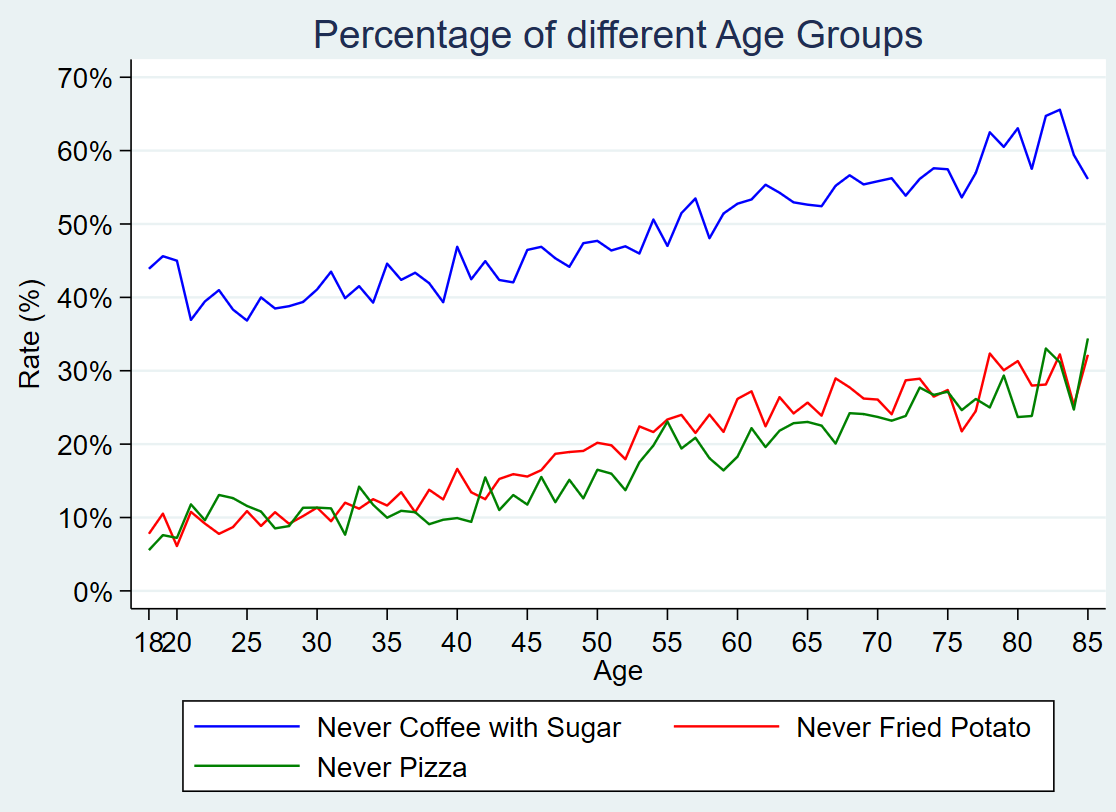
\includegraphics[width=\textwidth]{../Image/Graph01.png}
		\caption{Percentage of different age groups who never drink non-sugar coffee or tee, eat fried potatos or eat pizza}
		\label{fig:G1}
	\end{minipage}
	\hfill
	\begin{minipage}[b]{0.45\linewidth}
		\centering
		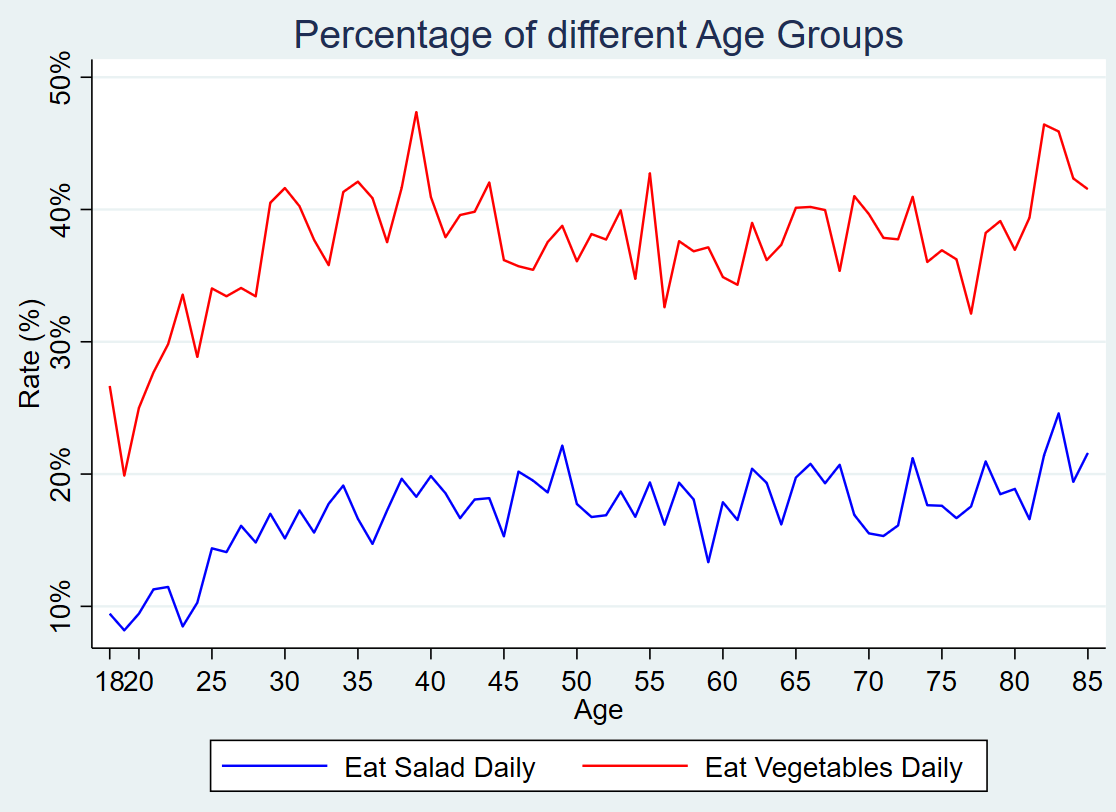
\includegraphics[width=\textwidth]{../Image/Graph02.png}
		\caption{Percentage of different age groups who eat salad daily or eat vegetables daily}
		\label{fig:G2}
	\end{minipage}
\end{figure}

The difference in lifestyle habits is also obvious in gender. The proportion of men who never drink pure fruit juice(41.49\%) is significantly lower than women(50.10\%), while the proportion of women who do not drink coffee or tee with sugar(46.97\%) is also slightly lower than men(51.86\%). In the case of salads and vegetables, the proportion of women(salad 19.83\% vegatables 42.37\%) who ate them every day was also higher than men(salad 14.69\% vegetables 32.27\%). We can see the gender differences in eating habits more directly by looking at the bar charts below.


\begin{figure}[!h]
	\centering
	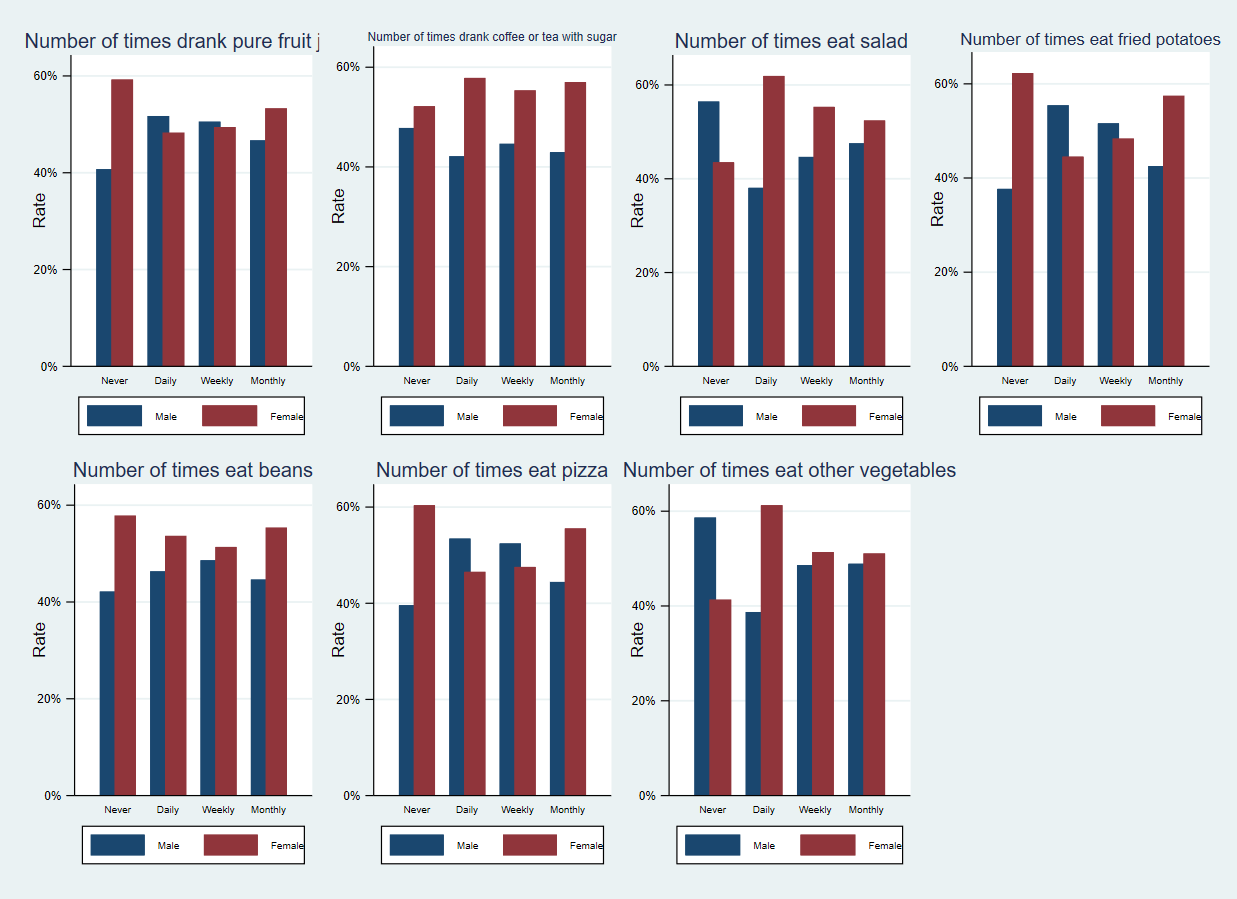
\includegraphics[width=0.9\textwidth]{../Image/Graph03.png}
	\caption{Comparison of Dietary Differences between Men and Women}
	\label{fig:G3}
\end{figure}


Similar differences can also be observed when examining race, housing status, and region in Table 2, reflecting how these factors may influence dietary habits among populations.



\subsection{Cardiovascular Conditions with Demographics}

From Table 1, we could get some rough findings. The percentage of the population who was diagnosed with caediovascular the conditions increases with age. For example, the percentage of coronary heart disease for people over 80 years old is 20.42\%, and the percentage for people between 18 and 40 years old is only 0.33\%. As shown in the figure below, the prevalence of various cardiovascular diseases has shown a significant increasing trend. This suggests that age is an important risk factor with important implications for cardiovascular health management and prevention strategies.

\begin{figure}[!h]
	\centering
	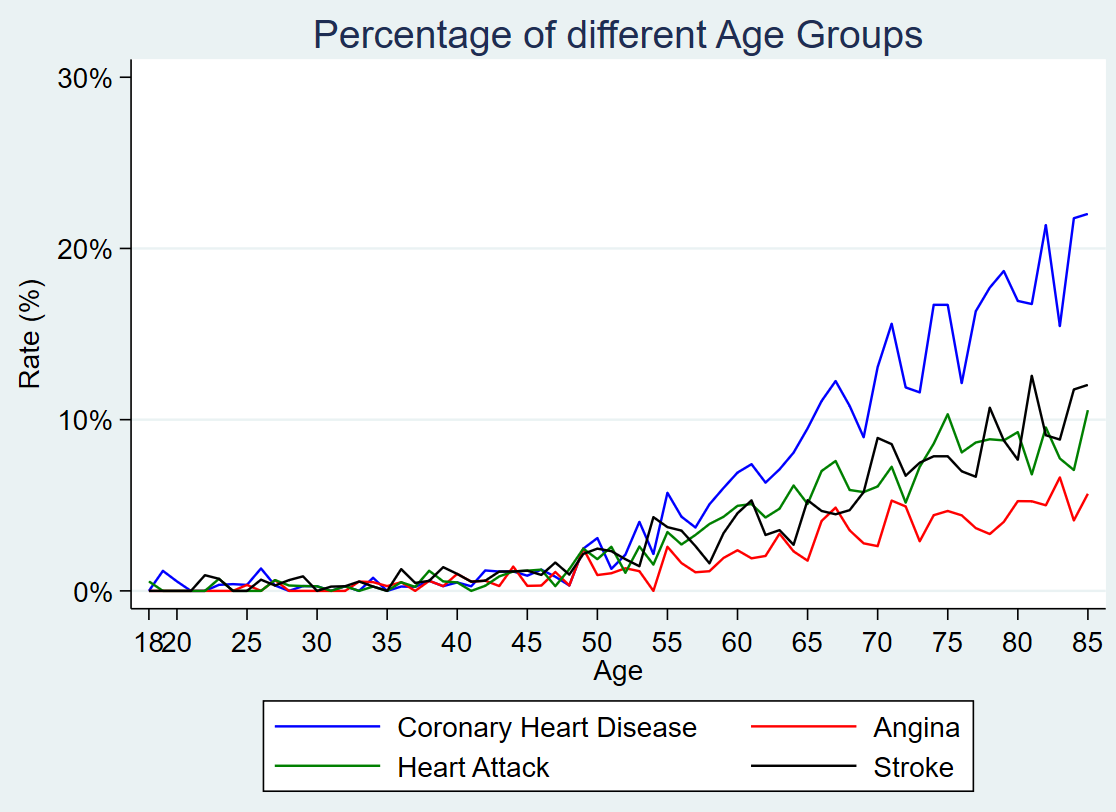
\includegraphics[width=0.4\textwidth]{../Image/Graph04.png}
	\caption{Comparison of Diseases Differences of Different Age}
	\label{fig:G4}
\end{figure}

Cardiovascular disease also has some race differencces, with American Indians or Alaska Natives having a higher cardiovascular prevalence than other races. For example, the the diagnosis rate for coronary heart disease is 7.42\% for American Indians or Alaska Natives compared to 3.39\% for the Asian group. This may reflect genetic factors, cultural practices, or an uneven distribution of health care resources. 

In terms of sex, except stroke(female were slightly higher by 0.3\%), all the other three cardiovascular diseases have a higher group rate of male than female. This may be related to biological sex differences, lifestyle choices, or other health factors and deserves further exploration.

In addition, we can also use the chi-square test method to determine whether the variables are statistically related. The following two images are Chi-square test results showing a statistical association between gender and coronary heart disease and no significant association between gender and stroke.

\begin{figure}[!h]   
	\begin{minipage}[b]{0.45\linewidth}
		\centering
		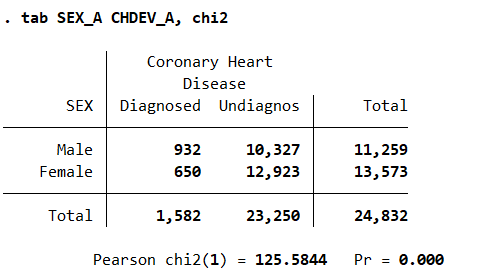
\includegraphics[width=\textwidth]{../Image/Chi2_S1.png}
		\caption{Sex-Coronary Chi-square test}
		\label{fig:S1}
	\end{minipage}
	\hfill
	\begin{minipage}[b]{0.45\linewidth}
		\centering
		\includegraphics[width=\textwidth]{../Image/CHi2_S2.png}
		\caption{Sex-Stroke Chi-square test}
		\label{fig:S2}
	\end{minipage}
\end{figure}

Take the second Chi-square test as an example, Pearson chi2(1) = 1.5553: This value is the Pearson Chi-square statistic, which measures the degree of deviation between the observed data and the expected data. The value of the statistic is relatively small, indicating that the observed data does not differ much from the expected data. Pr = 0.212: The size of this p-value is used to evaluate the significance of the statistical results. Here, a P-value of 0.212 is greater than the usual level of significance (e.g. 0.05), indicating that the observed association between sex and stroke is not statistically significant.

In terms of residence, if we go to the statistics of the population diagnosed with coronary heart disease, which type of people account for a large proportion, as shown in the figure below. We will find that the probability of coronary heart disease in homeowners is much higher than that in renters. However, this is due to the fact that there are nearly twice as many homeowners as renters in the statistics, so a large number of people surveyed with coronary heart disease were homeowners. In fact, by observing Table 1, we can find that the diagnosis rate of coronary heart disease among homeowners (6.84\%) is only slightly higher than that of renters (5.0\%), while the diagnosis rates of the other three diseases are basically the same in the two groups. The extent to which the type of residence had an effect on the presence or absence of a disease was not obvious.


\begin{figure}[!h]
	\centering
	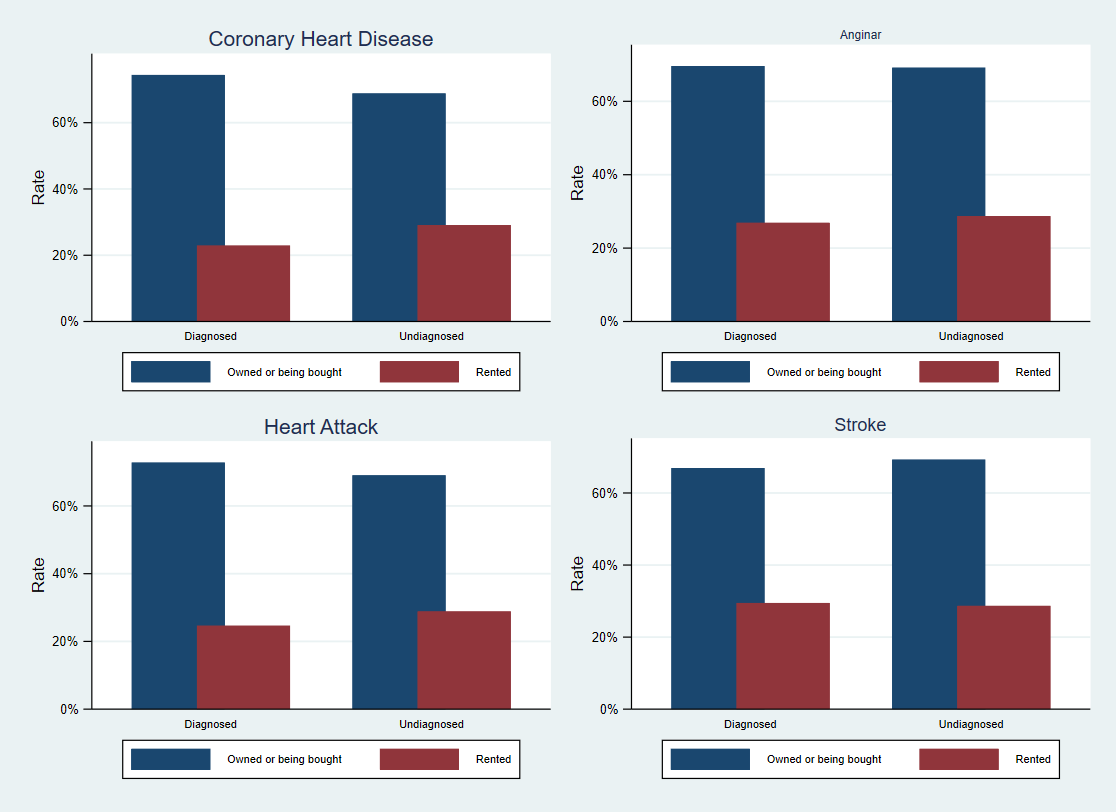
\includegraphics[width=0.5\textwidth]{../Image/Graph05.png}
	\caption{Proportion of Residence Types in the Coronary Heart Disease Population}
	\label{fig:G4}
\end{figure}

Regarding region we found that coronary heart disease was significantly less to be diagnosed in those living in the west(4.87\%) than those living in other regions. It may be related to the specific environment, dietary habits or socioeconomic factors in the region.

\newpage
\section{Task 3}
In order to explore the relationship among lifestyle habits, BMI, and coronary heart disease, I try to visually present the results using tables by combining various conditions. For example, the proportion of people who never eat vegetables, pizza, or fried potatoes who have coronary heart disease or are obese can be found in Tables 3 and 5.

However, the actual value of these probabilities is influenced by the sample size. As we can see from Tables 4 and 6, after applying multiple conditions, the number of people meeting certain criteria is too small, making the probabilities too random to derive any universal patterns. And if we want to refer to more types of data, this method makes the table very long and difficult to read.

When exploring significant correlations between variables, we continue to use the chi-square test as demonstrated in Task 2, looking at the magnitude of the p's value versus 0.05 to determine if the hypothesis is met and to determine if the variables are significant.

Therefore, I am considering using a more standardized statistical method, such as logistic regression analysis, to conduct a more rigorous analysis and reduce the impact of noise in the dataset. It should be noted that the binary output of stata's logistic regression must be 0 or 1, and the diagnosis and undiagnosis of cardiovascular disease in our codebook are 1 and 2, and a 2-to-0 preprocessing is required. And as for the variable of eating frequency we used, 1 is never,2 is daily,3 is weekly and 4monthly. We should reorder it according to the increasing frequency of eating from not eating to eating. In addition, logistic regression is not applicable when studying BMI, because BMI has four outcomes rather than binary variables. So I consider using ordered logistic regression models.

In addition to the above model, I also consider introducing other statistical algorithms and models, to help us more comprehensive understanding of the data, and make predictions. KNN, Decision Tree, Random Forest and CatBoost are commonly used models in machine learning.KNN it's K value represents the number of nearest neighbors selected and KNN decides the category or predicted value of the new data point based on the category of these neighbors.KNN is simple and intuitive but computationally expensive on large data sets and performs poorly on noisy and high dimensional data. Decision tree is a tree-structured model where each node represents a feature, branches represent feature values, and leaf nodes represent categories or regression values. It constructs a tree model by recursively selecting the optimal features to partition the dataset. However, it is prone to overfitting and sensitive to noisy data. Random forest is an integrated learning method that obtains the final result by generating multiple decision trees and voting or averaging their predictions. However, it has a long training and prediction time and high model complexity.CatBoost is an algorithm based on Gradient Boosted Decision Trees (GBDT) that is particularly good at handling categorical features. It reduces the risk of overfitting by converting categorical features to numerical features and using mean coding.CatBoost processes categorical features automatically, reducing the need for manual feature engineering, and performs well with datasets containing a large number of categorical features. However, the model is complex, difficult to interpret, and requires extensive parameter tuning.

\newpage
\thispagestyle {empty}
\begin{table}[!h]
	\centering
	\scalebox{0.5}{
			\begin{tabular}{lllllllll}
				\cline{1-9}
				\multicolumn{1}{c}{} &
				\multicolumn{2}{|c}{Coronary Heart Disease} &
				\multicolumn{2}{c}{Angina} &
				\multicolumn{2}{c}{Heart Attack} &
				\multicolumn{2}{c}{Stroke} \\
				\multicolumn{1}{c}{} &
				\multicolumn{1}{|r}{Diagnosed} &
				\multicolumn{1}{r}{Undiagnosed} &
				\multicolumn{1}{r}{Diagnosed} &
				\multicolumn{1}{r}{Undiagnosed} &
				\multicolumn{1}{r}{Diagnosed} &
				\multicolumn{1}{r}{Undiagnosed} &
				\multicolumn{1}{r}{Diagnosed} &
				\multicolumn{1}{r}{Undiagnosed} \\
				\cline{1-9}
				\multicolumn{1}{l}{Number of times eat other vegetables} &
				\multicolumn{1}{|r}{} &
				\multicolumn{1}{r}{} &
				\multicolumn{1}{r}{} &
				\multicolumn{1}{r}{} &
				\multicolumn{1}{r}{} &
				\multicolumn{1}{r}{} &
				\multicolumn{1}{r}{} &
				\multicolumn{1}{r}{} \\
				\multicolumn{1}{l}{\hspace{1em}Never} &
				\multicolumn{1}{|r}{} &
				\multicolumn{1}{r}{} &
				\multicolumn{1}{r}{} &
				\multicolumn{1}{r}{} &
				\multicolumn{1}{r}{} &
				\multicolumn{1}{r}{} &
				\multicolumn{1}{r}{} &
				\multicolumn{1}{r}{} \\
				\multicolumn{1}{l}{\hspace{2em}Number of times eat pizza} &
				\multicolumn{1}{|r}{} &
				\multicolumn{1}{r}{} &
				\multicolumn{1}{r}{} &
				\multicolumn{1}{r}{} &
				\multicolumn{1}{r}{} &
				\multicolumn{1}{r}{} &
				\multicolumn{1}{r}{} &
				\multicolumn{1}{r}{} \\
				\multicolumn{1}{l}{\hspace{3em}Never} &
				\multicolumn{1}{|r}{} &
				\multicolumn{1}{r}{} &
				\multicolumn{1}{r}{} &
				\multicolumn{1}{r}{} &
				\multicolumn{1}{r}{} &
				\multicolumn{1}{r}{} &
				\multicolumn{1}{r}{} &
				\multicolumn{1}{r}{} \\
				\multicolumn{1}{l}{\hspace{4em}Number of times eat fried potatoes} &
				\multicolumn{1}{|r}{} &
				\multicolumn{1}{r}{} &
				\multicolumn{1}{r}{} &
				\multicolumn{1}{r}{} &
				\multicolumn{1}{r}{} &
				\multicolumn{1}{r}{} &
				\multicolumn{1}{r}{} &
				\multicolumn{1}{r}{} \\
				\multicolumn{1}{l}{\hspace{5em}Never} &
				\multicolumn{1}{|r}{11.42857} &
				\multicolumn{1}{r}{88.57143} &
				\multicolumn{1}{r}{2.142857} &
				\multicolumn{1}{r}{97.85714} &
				\multicolumn{1}{r}{6.428571} &
				\multicolumn{1}{r}{93.57143} &
				\multicolumn{1}{r}{7.142857} &
				\multicolumn{1}{r}{92.85714} \\
				\multicolumn{1}{l}{\hspace{5em}Daily} &
				\multicolumn{1}{|r}{} &
				\multicolumn{1}{r}{100} &
				\multicolumn{1}{r}{} &
				\multicolumn{1}{r}{100} &
				\multicolumn{1}{r}{7.142857} &
				\multicolumn{1}{r}{92.85714} &
				\multicolumn{1}{r}{7.142857} &
				\multicolumn{1}{r}{92.85714} \\
				\multicolumn{1}{l}{\hspace{5em}Weekly} &
				\multicolumn{1}{|r}{6.557377} &
				\multicolumn{1}{r}{93.44262} &
				\multicolumn{1}{r}{3.278689} &
				\multicolumn{1}{r}{96.72131} &
				\multicolumn{1}{r}{8.196721} &
				\multicolumn{1}{r}{91.80328} &
				\multicolumn{1}{r}{9.836066} &
				\multicolumn{1}{r}{90.16393} \\
				\multicolumn{1}{l}{\hspace{5em}Monthly} &
				\multicolumn{1}{|r}{7.8125} &
				\multicolumn{1}{r}{92.1875} &
				\multicolumn{1}{r}{4.6875} &
				\multicolumn{1}{r}{95.3125} &
				\multicolumn{1}{r}{1.5625} &
				\multicolumn{1}{r}{98.4375} &
				\multicolumn{1}{r}{7.8125} &
				\multicolumn{1}{r}{92.1875} \\
				\multicolumn{1}{l}{\hspace{3em}Daily} &
				\multicolumn{1}{|r}{} &
				\multicolumn{1}{r}{} &
				\multicolumn{1}{r}{} &
				\multicolumn{1}{r}{} &
				\multicolumn{1}{r}{} &
				\multicolumn{1}{r}{} &
				\multicolumn{1}{r}{} &
				\multicolumn{1}{r}{} \\
				\multicolumn{1}{l}{\hspace{4em}Number of times eat fried potatoes} &
				\multicolumn{1}{|r}{} &
				\multicolumn{1}{r}{} &
				\multicolumn{1}{r}{} &
				\multicolumn{1}{r}{} &
				\multicolumn{1}{r}{} &
				\multicolumn{1}{r}{} &
				\multicolumn{1}{r}{} &
				\multicolumn{1}{r}{} \\
				\multicolumn{1}{l}{\hspace{5em}Never} &
				\multicolumn{1}{|r}{} &
				\multicolumn{1}{r}{100} &
				\multicolumn{1}{r}{} &
				\multicolumn{1}{r}{100} &
				\multicolumn{1}{r}{} &
				\multicolumn{1}{r}{100} &
				\multicolumn{1}{r}{} &
				\multicolumn{1}{r}{100} \\
				\multicolumn{1}{l}{\hspace{5em}Daily} &
				\multicolumn{1}{|r}{} &
				\multicolumn{1}{r}{100} &
				\multicolumn{1}{r}{} &
				\multicolumn{1}{r}{100} &
				\multicolumn{1}{r}{} &
				\multicolumn{1}{r}{100} &
				\multicolumn{1}{r}{} &
				\multicolumn{1}{r}{100} \\
				\multicolumn{1}{l}{\hspace{5em}Weekly} &
				\multicolumn{1}{|r}{} &
				\multicolumn{1}{r}{100} &
				\multicolumn{1}{r}{} &
				\multicolumn{1}{r}{100} &
				\multicolumn{1}{r}{} &
				\multicolumn{1}{r}{100} &
				\multicolumn{1}{r}{} &
				\multicolumn{1}{r}{100} \\
				\multicolumn{1}{l}{\hspace{5em}Monthly} &
				\multicolumn{1}{|r}{} &
				\multicolumn{1}{r}{100} &
				\multicolumn{1}{r}{} &
				\multicolumn{1}{r}{100} &
				\multicolumn{1}{r}{} &
				\multicolumn{1}{r}{100} &
				\multicolumn{1}{r}{} &
				\multicolumn{1}{r}{100} \\
				\multicolumn{1}{l}{\hspace{3em}Weekly} &
				\multicolumn{1}{|r}{} &
				\multicolumn{1}{r}{} &
				\multicolumn{1}{r}{} &
				\multicolumn{1}{r}{} &
				\multicolumn{1}{r}{} &
				\multicolumn{1}{r}{} &
				\multicolumn{1}{r}{} &
				\multicolumn{1}{r}{} \\
				\multicolumn{1}{l}{\hspace{4em}Number of times eat fried potatoes} &
				\multicolumn{1}{|r}{} &
				\multicolumn{1}{r}{} &
				\multicolumn{1}{r}{} &
				\multicolumn{1}{r}{} &
				\multicolumn{1}{r}{} &
				\multicolumn{1}{r}{} &
				\multicolumn{1}{r}{} &
				\multicolumn{1}{r}{} \\
				\multicolumn{1}{l}{\hspace{5em}Never} &
				\multicolumn{1}{|r}{12} &
				\multicolumn{1}{r}{88} &
				\multicolumn{1}{r}{} &
				\multicolumn{1}{r}{100} &
				\multicolumn{1}{r}{8} &
				\multicolumn{1}{r}{92} &
				\multicolumn{1}{r}{} &
				\multicolumn{1}{r}{100} \\
				\multicolumn{1}{l}{\hspace{5em}Daily} &
				\multicolumn{1}{|r}{} &
				\multicolumn{1}{r}{100} &
				\multicolumn{1}{r}{6.666667} &
				\multicolumn{1}{r}{93.33333} &
				\multicolumn{1}{r}{6.666667} &
				\multicolumn{1}{r}{93.33333} &
				\multicolumn{1}{r}{13.33333} &
				\multicolumn{1}{r}{86.66667} \\
				\multicolumn{1}{l}{\hspace{5em}Weekly} &
				\multicolumn{1}{|r}{8.275862} &
				\multicolumn{1}{r}{91.72414} &
				\multicolumn{1}{r}{1.37931} &
				\multicolumn{1}{r}{98.62069} &
				\multicolumn{1}{r}{1.37931} &
				\multicolumn{1}{r}{98.62069} &
				\multicolumn{1}{r}{2.068966} &
				\multicolumn{1}{r}{97.93103} \\
				\multicolumn{1}{l}{\hspace{5em}Monthly} &
				\multicolumn{1}{|r}{5.555556} &
				\multicolumn{1}{r}{94.44444} &
				\multicolumn{1}{r}{2.777778} &
				\multicolumn{1}{r}{97.22222} &
				\multicolumn{1}{r}{2.777778} &
				\multicolumn{1}{r}{97.22222} &
				\multicolumn{1}{r}{11.11111} &
				\multicolumn{1}{r}{88.88889} \\
				\multicolumn{1}{l}{\hspace{3em}Monthly} &
				\multicolumn{1}{|r}{} &
				\multicolumn{1}{r}{} &
				\multicolumn{1}{r}{} &
				\multicolumn{1}{r}{} &
				\multicolumn{1}{r}{} &
				\multicolumn{1}{r}{} &
				\multicolumn{1}{r}{} &
				\multicolumn{1}{r}{} \\
				\multicolumn{1}{l}{\hspace{4em}Number of times eat fried potatoes} &
				\multicolumn{1}{|r}{} &
				\multicolumn{1}{r}{} &
				\multicolumn{1}{r}{} &
				\multicolumn{1}{r}{} &
				\multicolumn{1}{r}{} &
				\multicolumn{1}{r}{} &
				\multicolumn{1}{r}{} &
				\multicolumn{1}{r}{} \\
				\multicolumn{1}{l}{\hspace{5em}Never} &
				\multicolumn{1}{|r}{7.070707} &
				\multicolumn{1}{r}{92.92929} &
				\multicolumn{1}{r}{3.030303} &
				\multicolumn{1}{r}{96.9697} &
				\multicolumn{1}{r}{6.060606} &
				\multicolumn{1}{r}{93.93939} &
				\multicolumn{1}{r}{3.030303} &
				\multicolumn{1}{r}{96.9697} \\
				\multicolumn{1}{l}{\hspace{5em}Daily} &
				\multicolumn{1}{|r}{22.22222} &
				\multicolumn{1}{r}{77.77778} &
				\multicolumn{1}{r}{5.555556} &
				\multicolumn{1}{r}{94.44444} &
				\multicolumn{1}{r}{11.11111} &
				\multicolumn{1}{r}{88.88889} &
				\multicolumn{1}{r}{16.66667} &
				\multicolumn{1}{r}{83.33333} \\
				\multicolumn{1}{l}{\hspace{5em}Weekly} &
				\multicolumn{1}{|r}{10.17964} &
				\multicolumn{1}{r}{89.82036} &
				\multicolumn{1}{r}{1.197605} &
				\multicolumn{1}{r}{98.8024} &
				\multicolumn{1}{r}{4.790419} &
				\multicolumn{1}{r}{95.20958} &
				\multicolumn{1}{r}{3.592814} &
				\multicolumn{1}{r}{96.40719} \\
				\multicolumn{1}{l}{\hspace{5em}Monthly} &
				\multicolumn{1}{|r}{5.970149} &
				\multicolumn{1}{r}{94.02985} &
				\multicolumn{1}{r}{1.99005} &
				\multicolumn{1}{r}{98.00995} &
				\multicolumn{1}{r}{3.482587} &
				\multicolumn{1}{r}{96.51741} &
				\multicolumn{1}{r}{3.9801} &
				\multicolumn{1}{r}{96.0199} \\
				\multicolumn{1}{l}{\hspace{1em}Daily} &
				\multicolumn{1}{|r}{} &
				\multicolumn{1}{r}{} &
				\multicolumn{1}{r}{} &
				\multicolumn{1}{r}{} &
				\multicolumn{1}{r}{} &
				\multicolumn{1}{r}{} &
				\multicolumn{1}{r}{} &
				\multicolumn{1}{r}{} \\
				\multicolumn{1}{l}{\hspace{2em}Number of times eat pizza} &
				\multicolumn{1}{|r}{} &
				\multicolumn{1}{r}{} &
				\multicolumn{1}{r}{} &
				\multicolumn{1}{r}{} &
				\multicolumn{1}{r}{} &
				\multicolumn{1}{r}{} &
				\multicolumn{1}{r}{} &
				\multicolumn{1}{r}{} \\
				\multicolumn{1}{l}{\hspace{3em}Never} &
				\multicolumn{1}{|r}{} &
				\multicolumn{1}{r}{} &
				\multicolumn{1}{r}{} &
				\multicolumn{1}{r}{} &
				\multicolumn{1}{r}{} &
				\multicolumn{1}{r}{} &
				\multicolumn{1}{r}{} &
				\multicolumn{1}{r}{} \\
				\multicolumn{1}{l}{\hspace{4em}Number of times eat fried potatoes} &
				\multicolumn{1}{|r}{} &
				\multicolumn{1}{r}{} &
				\multicolumn{1}{r}{} &
				\multicolumn{1}{r}{} &
				\multicolumn{1}{r}{} &
				\multicolumn{1}{r}{} &
				\multicolumn{1}{r}{} &
				\multicolumn{1}{r}{} \\
				\multicolumn{1}{l}{\hspace{5em}Never} &
				\multicolumn{1}{|r}{7.182941} &
				\multicolumn{1}{r}{92.81706} &
				\multicolumn{1}{r}{2.469136} &
				\multicolumn{1}{r}{97.53086} &
				\multicolumn{1}{r}{4.040404} &
				\multicolumn{1}{r}{95.9596} &
				\multicolumn{1}{r}{3.928171} &
				\multicolumn{1}{r}{96.07183} \\
				\multicolumn{1}{l}{\hspace{5em}Daily} &
				\multicolumn{1}{|r}{18.75} &
				\multicolumn{1}{r}{81.25} &
				\multicolumn{1}{r}{} &
				\multicolumn{1}{r}{100} &
				\multicolumn{1}{r}{} &
				\multicolumn{1}{r}{100} &
				\multicolumn{1}{r}{9.375} &
				\multicolumn{1}{r}{90.625} \\
				\multicolumn{1}{l}{\hspace{5em}Weekly} &
				\multicolumn{1}{|r}{4.968944} &
				\multicolumn{1}{r}{95.03106} &
				\multicolumn{1}{r}{2.484472} &
				\multicolumn{1}{r}{97.51553} &
				\multicolumn{1}{r}{3.416149} &
				\multicolumn{1}{r}{96.58385} &
				\multicolumn{1}{r}{3.416149} &
				\multicolumn{1}{r}{96.58385} \\
				\multicolumn{1}{l}{\hspace{5em}Monthly} &
				\multicolumn{1}{|r}{8.073394} &
				\multicolumn{1}{r}{91.92661} &
				\multicolumn{1}{r}{2.385321} &
				\multicolumn{1}{r}{97.61468} &
				\multicolumn{1}{r}{5.321101} &
				\multicolumn{1}{r}{94.6789} &
				\multicolumn{1}{r}{3.119266} &
				\multicolumn{1}{r}{96.88073} \\
				\multicolumn{1}{l}{\hspace{3em}Daily} &
				\multicolumn{1}{|r}{} &
				\multicolumn{1}{r}{} &
				\multicolumn{1}{r}{} &
				\multicolumn{1}{r}{} &
				\multicolumn{1}{r}{} &
				\multicolumn{1}{r}{} &
				\multicolumn{1}{r}{} &
				\multicolumn{1}{r}{} \\
				\multicolumn{1}{l}{\hspace{4em}Number of times eat fried potatoes} &
				\multicolumn{1}{|r}{} &
				\multicolumn{1}{r}{} &
				\multicolumn{1}{r}{} &
				\multicolumn{1}{r}{} &
				\multicolumn{1}{r}{} &
				\multicolumn{1}{r}{} &
				\multicolumn{1}{r}{} &
				\multicolumn{1}{r}{} \\
				\multicolumn{1}{l}{\hspace{5em}Never} &
				\multicolumn{1}{|r}{15.38462} &
				\multicolumn{1}{r}{84.61538} &
				\multicolumn{1}{r}{} &
				\multicolumn{1}{r}{100} &
				\multicolumn{1}{r}{} &
				\multicolumn{1}{r}{100} &
				\multicolumn{1}{r}{} &
				\multicolumn{1}{r}{100} \\
				\multicolumn{1}{l}{\hspace{5em}Daily} &
				\multicolumn{1}{|r}{9.677419} &
				\multicolumn{1}{r}{90.32258} &
				\multicolumn{1}{r}{3.225806} &
				\multicolumn{1}{r}{96.77419} &
				\multicolumn{1}{r}{3.225806} &
				\multicolumn{1}{r}{96.77419} &
				\multicolumn{1}{r}{9.677419} &
				\multicolumn{1}{r}{90.32258} \\
				\multicolumn{1}{l}{\hspace{5em}Weekly} &
				\multicolumn{1}{|r}{} &
				\multicolumn{1}{r}{100} &
				\multicolumn{1}{r}{} &
				\multicolumn{1}{r}{100} &
				\multicolumn{1}{r}{} &
				\multicolumn{1}{r}{100} &
				\multicolumn{1}{r}{} &
				\multicolumn{1}{r}{100} \\
				\multicolumn{1}{l}{\hspace{5em}Monthly} &
				\multicolumn{1}{|r}{18.75} &
				\multicolumn{1}{r}{81.25} &
				\multicolumn{1}{r}{6.25} &
				\multicolumn{1}{r}{93.75} &
				\multicolumn{1}{r}{} &
				\multicolumn{1}{r}{100} &
				\multicolumn{1}{r}{6.25} &
				\multicolumn{1}{r}{93.75} \\
				\multicolumn{1}{l}{\hspace{3em}Weekly} &
				\multicolumn{1}{|r}{} &
				\multicolumn{1}{r}{} &
				\multicolumn{1}{r}{} &
				\multicolumn{1}{r}{} &
				\multicolumn{1}{r}{} &
				\multicolumn{1}{r}{} &
				\multicolumn{1}{r}{} &
				\multicolumn{1}{r}{} \\
				\multicolumn{1}{l}{\hspace{4em}Number of times eat fried potatoes} &
				\multicolumn{1}{|r}{} &
				\multicolumn{1}{r}{} &
				\multicolumn{1}{r}{} &
				\multicolumn{1}{r}{} &
				\multicolumn{1}{r}{} &
				\multicolumn{1}{r}{} &
				\multicolumn{1}{r}{} &
				\multicolumn{1}{r}{} \\
				\multicolumn{1}{l}{\hspace{5em}Never} &
				\multicolumn{1}{|r}{6.477733} &
				\multicolumn{1}{r}{93.52227} &
				\multicolumn{1}{r}{2.42915} &
				\multicolumn{1}{r}{97.57085} &
				\multicolumn{1}{r}{3.238866} &
				\multicolumn{1}{r}{96.76113} &
				\multicolumn{1}{r}{3.238866} &
				\multicolumn{1}{r}{96.76113} \\
				\multicolumn{1}{l}{\hspace{5em}Daily} &
				\multicolumn{1}{|r}{2.272727} &
				\multicolumn{1}{r}{97.72727} &
				\multicolumn{1}{r}{2.272727} &
				\multicolumn{1}{r}{97.72727} &
				\multicolumn{1}{r}{3.409091} &
				\multicolumn{1}{r}{96.59091} &
				\multicolumn{1}{r}{2.272727} &
				\multicolumn{1}{r}{97.72727} \\
				\multicolumn{1}{l}{\hspace{5em}Weekly} &
				\multicolumn{1}{|r}{4.036697} &
				\multicolumn{1}{r}{95.9633} &
				\multicolumn{1}{r}{1.651376} &
				\multicolumn{1}{r}{98.34862} &
				\multicolumn{1}{r}{2.385321} &
				\multicolumn{1}{r}{97.61468} &
				\multicolumn{1}{r}{2.568807} &
				\multicolumn{1}{r}{97.43119} \\
				\multicolumn{1}{l}{\hspace{5em}Monthly} &
				\multicolumn{1}{|r}{4.139434} &
				\multicolumn{1}{r}{95.86057} &
				\multicolumn{1}{r}{1.960784} &
				\multicolumn{1}{r}{98.03922} &
				\multicolumn{1}{r}{2.396514} &
				\multicolumn{1}{r}{97.60349} &
				\multicolumn{1}{r}{3.267974} &
				\multicolumn{1}{r}{96.73203} \\
				\multicolumn{1}{l}{\hspace{3em}Monthly} &
				\multicolumn{1}{|r}{} &
				\multicolumn{1}{r}{} &
				\multicolumn{1}{r}{} &
				\multicolumn{1}{r}{} &
				\multicolumn{1}{r}{} &
				\multicolumn{1}{r}{} &
				\multicolumn{1}{r}{} &
				\multicolumn{1}{r}{} \\
				\multicolumn{1}{l}{\hspace{4em}Number of times eat fried potatoes} &
				\multicolumn{1}{|r}{} &
				\multicolumn{1}{r}{} &
				\multicolumn{1}{r}{} &
				\multicolumn{1}{r}{} &
				\multicolumn{1}{r}{} &
				\multicolumn{1}{r}{} &
				\multicolumn{1}{r}{} &
				\multicolumn{1}{r}{} \\
				\multicolumn{1}{l}{\hspace{5em}Never} &
				\multicolumn{1}{|r}{6.325301} &
				\multicolumn{1}{r}{93.6747} &
				\multicolumn{1}{r}{2.108434} &
				\multicolumn{1}{r}{97.89157} &
				\multicolumn{1}{r}{3.012048} &
				\multicolumn{1}{r}{96.98795} &
				\multicolumn{1}{r}{4.417671} &
				\multicolumn{1}{r}{95.58233} \\
				\multicolumn{1}{l}{\hspace{5em}Daily} &
				\multicolumn{1}{|r}{7.758621} &
				\multicolumn{1}{r}{92.24138} &
				\multicolumn{1}{r}{4.310345} &
				\multicolumn{1}{r}{95.68966} &
				\multicolumn{1}{r}{7.758621} &
				\multicolumn{1}{r}{92.24138} &
				\multicolumn{1}{r}{5.172414} &
				\multicolumn{1}{r}{94.82759} \\
				\multicolumn{1}{l}{\hspace{5em}Weekly} &
				\multicolumn{1}{|r}{6.081081} &
				\multicolumn{1}{r}{93.91892} &
				\multicolumn{1}{r}{1.689189} &
				\multicolumn{1}{r}{98.31081} &
				\multicolumn{1}{r}{3.65991} &
				\multicolumn{1}{r}{96.34009} &
				\multicolumn{1}{r}{3.153153} &
				\multicolumn{1}{r}{96.84685} \\
				\multicolumn{1}{l}{\hspace{5em}Monthly} &
				\multicolumn{1}{|r}{5.844418} &
				\multicolumn{1}{r}{94.15558} &
				\multicolumn{1}{r}{1.773478} &
				\multicolumn{1}{r}{98.22652} &
				\multicolumn{1}{r}{2.982668} &
				\multicolumn{1}{r}{97.01733} &
				\multicolumn{1}{r}{3.546957} &
				\multicolumn{1}{r}{96.45304} \\
				\multicolumn{1}{l}{\hspace{1em}Weekly} &
				\multicolumn{1}{|r}{} &
				\multicolumn{1}{r}{} &
				\multicolumn{1}{r}{} &
				\multicolumn{1}{r}{} &
				\multicolumn{1}{r}{} &
				\multicolumn{1}{r}{} &
				\multicolumn{1}{r}{} &
				\multicolumn{1}{r}{} \\
				\multicolumn{1}{l}{\hspace{2em}Number of times eat pizza} &
				\multicolumn{1}{|r}{} &
				\multicolumn{1}{r}{} &
				\multicolumn{1}{r}{} &
				\multicolumn{1}{r}{} &
				\multicolumn{1}{r}{} &
				\multicolumn{1}{r}{} &
				\multicolumn{1}{r}{} &
				\multicolumn{1}{r}{} \\
				\multicolumn{1}{l}{\hspace{3em}Never} &
				\multicolumn{1}{|r}{} &
				\multicolumn{1}{r}{} &
				\multicolumn{1}{r}{} &
				\multicolumn{1}{r}{} &
				\multicolumn{1}{r}{} &
				\multicolumn{1}{r}{} &
				\multicolumn{1}{r}{} &
				\multicolumn{1}{r}{} \\
				\multicolumn{1}{l}{\hspace{4em}Number of times eat fried potatoes} &
				\multicolumn{1}{|r}{} &
				\multicolumn{1}{r}{} &
				\multicolumn{1}{r}{} &
				\multicolumn{1}{r}{} &
				\multicolumn{1}{r}{} &
				\multicolumn{1}{r}{} &
				\multicolumn{1}{r}{} &
				\multicolumn{1}{r}{} \\
				\multicolumn{1}{l}{\hspace{5em}Never} &
				\multicolumn{1}{|r}{10.78014} &
				\multicolumn{1}{r}{89.21986} &
				\multicolumn{1}{r}{3.120567} &
				\multicolumn{1}{r}{96.87943} &
				\multicolumn{1}{r}{5.390071} &
				\multicolumn{1}{r}{94.60993} &
				\multicolumn{1}{r}{4.964539} &
				\multicolumn{1}{r}{95.03546} \\
				\multicolumn{1}{l}{\hspace{5em}Daily} &
				\multicolumn{1}{|r}{11.42857} &
				\multicolumn{1}{r}{88.57143} &
				\multicolumn{1}{r}{5.714286} &
				\multicolumn{1}{r}{94.28571} &
				\multicolumn{1}{r}{8.571429} &
				\multicolumn{1}{r}{91.42857} &
				\multicolumn{1}{r}{8.571429} &
				\multicolumn{1}{r}{91.42857} \\
				\multicolumn{1}{l}{\hspace{5em}Weekly} &
				\multicolumn{1}{|r}{8.350731} &
				\multicolumn{1}{r}{91.64927} &
				\multicolumn{1}{r}{3.131524} &
				\multicolumn{1}{r}{96.86848} &
				\multicolumn{1}{r}{4.80167} &
				\multicolumn{1}{r}{95.19833} &
				\multicolumn{1}{r}{5.845511} &
				\multicolumn{1}{r}{94.15449} \\
				\multicolumn{1}{l}{\hspace{5em}Monthly} &
				\multicolumn{1}{|r}{8.684864} &
				\multicolumn{1}{r}{91.31514} &
				\multicolumn{1}{r}{2.48139} &
				\multicolumn{1}{r}{97.51861} &
				\multicolumn{1}{r}{4.218362} &
				\multicolumn{1}{r}{95.78164} &
				\multicolumn{1}{r}{6.451613} &
				\multicolumn{1}{r}{93.54839} \\
				\multicolumn{1}{l}{\hspace{3em}Daily} &
				\multicolumn{1}{|r}{} &
				\multicolumn{1}{r}{} &
				\multicolumn{1}{r}{} &
				\multicolumn{1}{r}{} &
				\multicolumn{1}{r}{} &
				\multicolumn{1}{r}{} &
				\multicolumn{1}{r}{} &
				\multicolumn{1}{r}{} \\
				\multicolumn{1}{l}{\hspace{4em}Number of times eat fried potatoes} &
				\multicolumn{1}{|r}{} &
				\multicolumn{1}{r}{} &
				\multicolumn{1}{r}{} &
				\multicolumn{1}{r}{} &
				\multicolumn{1}{r}{} &
				\multicolumn{1}{r}{} &
				\multicolumn{1}{r}{} &
				\multicolumn{1}{r}{} \\
				\multicolumn{1}{l}{\hspace{5em}Never} &
				\multicolumn{1}{|r}{} &
				\multicolumn{1}{r}{100} &
				\multicolumn{1}{r}{} &
				\multicolumn{1}{r}{100} &
				\multicolumn{1}{r}{} &
				\multicolumn{1}{r}{100} &
				\multicolumn{1}{r}{11.11111} &
				\multicolumn{1}{r}{88.88889} \\
				\multicolumn{1}{l}{\hspace{5em}Daily} &
				\multicolumn{1}{|r}{20} &
				\multicolumn{1}{r}{80} &
				\multicolumn{1}{r}{} &
				\multicolumn{1}{r}{100} &
				\multicolumn{1}{r}{20} &
				\multicolumn{1}{r}{80} &
				\multicolumn{1}{r}{} &
				\multicolumn{1}{r}{100} \\
				\multicolumn{1}{l}{\hspace{5em}Weekly} &
				\multicolumn{1}{|r}{5.882353} &
				\multicolumn{1}{r}{94.11765} &
				\multicolumn{1}{r}{} &
				\multicolumn{1}{r}{100} &
				\multicolumn{1}{r}{} &
				\multicolumn{1}{r}{100} &
				\multicolumn{1}{r}{} &
				\multicolumn{1}{r}{100} \\
				\multicolumn{1}{l}{\hspace{5em}Monthly} &
				\multicolumn{1}{|r}{7.142857} &
				\multicolumn{1}{r}{92.85714} &
				\multicolumn{1}{r}{} &
				\multicolumn{1}{r}{100} &
				\multicolumn{1}{r}{7.142857} &
				\multicolumn{1}{r}{92.85714} &
				\multicolumn{1}{r}{14.28571} &
				\multicolumn{1}{r}{85.71429} \\
				\multicolumn{1}{l}{\hspace{3em}Weekly} &
				\multicolumn{1}{|r}{} &
				\multicolumn{1}{r}{} &
				\multicolumn{1}{r}{} &
				\multicolumn{1}{r}{} &
				\multicolumn{1}{r}{} &
				\multicolumn{1}{r}{} &
				\multicolumn{1}{r}{} &
				\multicolumn{1}{r}{} \\
				\multicolumn{1}{l}{\hspace{4em}Number of times eat fried potatoes} &
				\multicolumn{1}{|r}{} &
				\multicolumn{1}{r}{} &
				\multicolumn{1}{r}{} &
				\multicolumn{1}{r}{} &
				\multicolumn{1}{r}{} &
				\multicolumn{1}{r}{} &
				\multicolumn{1}{r}{} &
				\multicolumn{1}{r}{} \\
				\multicolumn{1}{l}{\hspace{5em}Never} &
				\multicolumn{1}{|r}{7.534247} &
				\multicolumn{1}{r}{92.46575} &
				\multicolumn{1}{r}{2.054795} &
				\multicolumn{1}{r}{97.94521} &
				\multicolumn{1}{r}{2.739726} &
				\multicolumn{1}{r}{97.26027} &
				\multicolumn{1}{r}{.6849315} &
				\multicolumn{1}{r}{99.31507} \\
				\multicolumn{1}{l}{\hspace{5em}Daily} &
				\multicolumn{1}{|r}{1.449275} &
				\multicolumn{1}{r}{98.55072} &
				\multicolumn{1}{r}{} &
				\multicolumn{1}{r}{100} &
				\multicolumn{1}{r}{} &
				\multicolumn{1}{r}{100} &
				\multicolumn{1}{r}{2.898551} &
				\multicolumn{1}{r}{97.10145} \\
				\multicolumn{1}{l}{\hspace{5em}Weekly} &
				\multicolumn{1}{|r}{4.579393} &
				\multicolumn{1}{r}{95.42061} &
				\multicolumn{1}{r}{1.692384} &
				\multicolumn{1}{r}{98.30762} &
				\multicolumn{1}{r}{2.887008} &
				\multicolumn{1}{r}{97.11299} &
				\multicolumn{1}{r}{2.588352} &
				\multicolumn{1}{r}{97.41165} \\
				\multicolumn{1}{l}{\hspace{5em}Monthly} &
				\multicolumn{1}{|r}{5.092593} &
				\multicolumn{1}{r}{94.90741} &
				\multicolumn{1}{r}{.6944444} &
				\multicolumn{1}{r}{99.30556} &
				\multicolumn{1}{r}{3.240741} &
				\multicolumn{1}{r}{96.75926} &
				\multicolumn{1}{r}{2.083333} &
				\multicolumn{1}{r}{97.91667} \\
				\multicolumn{1}{l}{\hspace{3em}Monthly} &
				\multicolumn{1}{|r}{} &
				\multicolumn{1}{r}{} &
				\multicolumn{1}{r}{} &
				\multicolumn{1}{r}{} &
				\multicolumn{1}{r}{} &
				\multicolumn{1}{r}{} &
				\multicolumn{1}{r}{} &
				\multicolumn{1}{r}{} \\
				\multicolumn{1}{l}{\hspace{4em}Number of times eat fried potatoes} &
				\multicolumn{1}{|r}{} &
				\multicolumn{1}{r}{} &
				\multicolumn{1}{r}{} &
				\multicolumn{1}{r}{} &
				\multicolumn{1}{r}{} &
				\multicolumn{1}{r}{} &
				\multicolumn{1}{r}{} &
				\multicolumn{1}{r}{} \\
				\multicolumn{1}{l}{\hspace{5em}Never} &
				\multicolumn{1}{|r}{8.041958} &
				\multicolumn{1}{r}{91.95804} &
				\multicolumn{1}{r}{1.864802} &
				\multicolumn{1}{r}{98.1352} &
				\multicolumn{1}{r}{3.962704} &
				\multicolumn{1}{r}{96.0373} &
				\multicolumn{1}{r}{4.079254} &
				\multicolumn{1}{r}{95.92075} \\
				\multicolumn{1}{l}{\hspace{5em}Daily} &
				\multicolumn{1}{|r}{7.936508} &
				\multicolumn{1}{r}{92.06349} &
				\multicolumn{1}{r}{4.761905} &
				\multicolumn{1}{r}{95.2381} &
				\multicolumn{1}{r}{3.174603} &
				\multicolumn{1}{r}{96.8254} &
				\multicolumn{1}{r}{3.174603} &
				\multicolumn{1}{r}{96.8254} \\
				\multicolumn{1}{l}{\hspace{5em}Weekly} &
				\multicolumn{1}{|r}{5.583174} &
				\multicolumn{1}{r}{94.41683} &
				\multicolumn{1}{r}{1.873805} &
				\multicolumn{1}{r}{98.1262} &
				\multicolumn{1}{r}{3.632887} &
				\multicolumn{1}{r}{96.36711} &
				\multicolumn{1}{r}{3.32696} &
				\multicolumn{1}{r}{96.67304} \\
				\multicolumn{1}{l}{\hspace{5em}Monthly} &
				\multicolumn{1}{|r}{6.483791} &
				\multicolumn{1}{r}{93.51621} &
				\multicolumn{1}{r}{1.795511} &
				\multicolumn{1}{r}{98.20449} &
				\multicolumn{1}{r}{3.541147} &
				\multicolumn{1}{r}{96.45885} &
				\multicolumn{1}{r}{2.942643} &
				\multicolumn{1}{r}{97.05736} \\
				\multicolumn{1}{l}{\hspace{1em}Monthly} &
				\multicolumn{1}{|r}{} &
				\multicolumn{1}{r}{} &
				\multicolumn{1}{r}{} &
				\multicolumn{1}{r}{} &
				\multicolumn{1}{r}{} &
				\multicolumn{1}{r}{} &
				\multicolumn{1}{r}{} &
				\multicolumn{1}{r}{} \\
				\multicolumn{1}{l}{\hspace{2em}Number of times eat pizza} &
				\multicolumn{1}{|r}{} &
				\multicolumn{1}{r}{} &
				\multicolumn{1}{r}{} &
				\multicolumn{1}{r}{} &
				\multicolumn{1}{r}{} &
				\multicolumn{1}{r}{} &
				\multicolumn{1}{r}{} &
				\multicolumn{1}{r}{} \\
				\multicolumn{1}{l}{\hspace{3em}Never} &
				\multicolumn{1}{|r}{} &
				\multicolumn{1}{r}{} &
				\multicolumn{1}{r}{} &
				\multicolumn{1}{r}{} &
				\multicolumn{1}{r}{} &
				\multicolumn{1}{r}{} &
				\multicolumn{1}{r}{} &
				\multicolumn{1}{r}{} \\
				\multicolumn{1}{l}{\hspace{4em}Number of times eat fried potatoes} &
				\multicolumn{1}{|r}{} &
				\multicolumn{1}{r}{} &
				\multicolumn{1}{r}{} &
				\multicolumn{1}{r}{} &
				\multicolumn{1}{r}{} &
				\multicolumn{1}{r}{} &
				\multicolumn{1}{r}{} &
				\multicolumn{1}{r}{} \\
				\multicolumn{1}{l}{\hspace{5em}Never} &
				\multicolumn{1}{|r}{10.94527} &
				\multicolumn{1}{r}{89.05473} &
				\multicolumn{1}{r}{2.487562} &
				\multicolumn{1}{r}{97.51244} &
				\multicolumn{1}{r}{8.955224} &
				\multicolumn{1}{r}{91.04478} &
				\multicolumn{1}{r}{7.960199} &
				\multicolumn{1}{r}{92.0398} \\
				\multicolumn{1}{l}{\hspace{5em}Daily} &
				\multicolumn{1}{|r}{40} &
				\multicolumn{1}{r}{60} &
				\multicolumn{1}{r}{20} &
				\multicolumn{1}{r}{80} &
				\multicolumn{1}{r}{20} &
				\multicolumn{1}{r}{80} &
				\multicolumn{1}{r}{20} &
				\multicolumn{1}{r}{80} \\
				\multicolumn{1}{l}{\hspace{5em}Weekly} &
				\multicolumn{1}{|r}{9.375} &
				\multicolumn{1}{r}{90.625} &
				\multicolumn{1}{r}{} &
				\multicolumn{1}{r}{100} &
				\multicolumn{1}{r}{7.8125} &
				\multicolumn{1}{r}{92.1875} &
				\multicolumn{1}{r}{4.6875} &
				\multicolumn{1}{r}{95.3125} \\
				\multicolumn{1}{l}{\hspace{5em}Monthly} &
				\multicolumn{1}{|r}{11.73184} &
				\multicolumn{1}{r}{88.26816} &
				\multicolumn{1}{r}{3.351955} &
				\multicolumn{1}{r}{96.64804} &
				\multicolumn{1}{r}{6.98324} &
				\multicolumn{1}{r}{93.01676} &
				\multicolumn{1}{r}{6.703911} &
				\multicolumn{1}{r}{93.29609} \\
				\multicolumn{1}{l}{\hspace{3em}Daily} &
				\multicolumn{1}{|r}{} &
				\multicolumn{1}{r}{} &
				\multicolumn{1}{r}{} &
				\multicolumn{1}{r}{} &
				\multicolumn{1}{r}{} &
				\multicolumn{1}{r}{} &
				\multicolumn{1}{r}{} &
				\multicolumn{1}{r}{} \\
				\multicolumn{1}{l}{\hspace{4em}Number of times eat fried potatoes} &
				\multicolumn{1}{|r}{} &
				\multicolumn{1}{r}{} &
				\multicolumn{1}{r}{} &
				\multicolumn{1}{r}{} &
				\multicolumn{1}{r}{} &
				\multicolumn{1}{r}{} &
				\multicolumn{1}{r}{} &
				\multicolumn{1}{r}{} \\
				\multicolumn{1}{l}{\hspace{5em}Never} &
				\multicolumn{1}{|r}{} &
				\multicolumn{1}{r}{100} &
				\multicolumn{1}{r}{} &
				\multicolumn{1}{r}{100} &
				\multicolumn{1}{r}{} &
				\multicolumn{1}{r}{100} &
				\multicolumn{1}{r}{} &
				\multicolumn{1}{r}{100} \\
				\multicolumn{1}{l}{\hspace{5em}Daily} &
				\multicolumn{1}{|r}{} &
				\multicolumn{1}{r}{100} &
				\multicolumn{1}{r}{} &
				\multicolumn{1}{r}{100} &
				\multicolumn{1}{r}{} &
				\multicolumn{1}{r}{100} &
				\multicolumn{1}{r}{} &
				\multicolumn{1}{r}{100} \\
				\multicolumn{1}{l}{\hspace{5em}Weekly} &
				\multicolumn{1}{|r}{} &
				\multicolumn{1}{r}{100} &
				\multicolumn{1}{r}{} &
				\multicolumn{1}{r}{100} &
				\multicolumn{1}{r}{25} &
				\multicolumn{1}{r}{75} &
				\multicolumn{1}{r}{} &
				\multicolumn{1}{r}{100} \\
				\multicolumn{1}{l}{\hspace{5em}Monthly} &
				\multicolumn{1}{|r}{} &
				\multicolumn{1}{r}{100} &
				\multicolumn{1}{r}{14.28571} &
				\multicolumn{1}{r}{85.71429} &
				\multicolumn{1}{r}{} &
				\multicolumn{1}{r}{100} &
				\multicolumn{1}{r}{14.28571} &
				\multicolumn{1}{r}{85.71429} \\
				\multicolumn{1}{l}{\hspace{3em}Weekly} &
				\multicolumn{1}{|r}{} &
				\multicolumn{1}{r}{} &
				\multicolumn{1}{r}{} &
				\multicolumn{1}{r}{} &
				\multicolumn{1}{r}{} &
				\multicolumn{1}{r}{} &
				\multicolumn{1}{r}{} &
				\multicolumn{1}{r}{} \\
				\multicolumn{1}{l}{\hspace{4em}Number of times eat fried potatoes} &
				\multicolumn{1}{|r}{} &
				\multicolumn{1}{r}{} &
				\multicolumn{1}{r}{} &
				\multicolumn{1}{r}{} &
				\multicolumn{1}{r}{} &
				\multicolumn{1}{r}{} &
				\multicolumn{1}{r}{} &
				\multicolumn{1}{r}{} \\
				\multicolumn{1}{l}{\hspace{5em}Never} &
				\multicolumn{1}{|r}{5.714286} &
				\multicolumn{1}{r}{94.28571} &
				\multicolumn{1}{r}{} &
				\multicolumn{1}{r}{100} &
				\multicolumn{1}{r}{5.714286} &
				\multicolumn{1}{r}{94.28571} &
				\multicolumn{1}{r}{5.714286} &
				\multicolumn{1}{r}{94.28571} \\
				\multicolumn{1}{l}{\hspace{5em}Daily} &
				\multicolumn{1}{|r}{9.090909} &
				\multicolumn{1}{r}{90.90909} &
				\multicolumn{1}{r}{} &
				\multicolumn{1}{r}{100} &
				\multicolumn{1}{r}{} &
				\multicolumn{1}{r}{100} &
				\multicolumn{1}{r}{} &
				\multicolumn{1}{r}{100} \\
				\multicolumn{1}{l}{\hspace{5em}Weekly} &
				\multicolumn{1}{|r}{3.703704} &
				\multicolumn{1}{r}{96.2963} &
				\multicolumn{1}{r}{1.851852} &
				\multicolumn{1}{r}{98.14815} &
				\multicolumn{1}{r}{2.469136} &
				\multicolumn{1}{r}{97.53086} &
				\multicolumn{1}{r}{2.469136} &
				\multicolumn{1}{r}{97.53086} \\
				\multicolumn{1}{l}{\hspace{5em}Monthly} &
				\multicolumn{1}{|r}{2.222222} &
				\multicolumn{1}{r}{97.77778} &
				\multicolumn{1}{r}{2.962963} &
				\multicolumn{1}{r}{97.03704} &
				\multicolumn{1}{r}{2.962963} &
				\multicolumn{1}{r}{97.03704} &
				\multicolumn{1}{r}{2.222222} &
				\multicolumn{1}{r}{97.77778} \\
				\multicolumn{1}{l}{\hspace{3em}Monthly} &
				\multicolumn{1}{|r}{} &
				\multicolumn{1}{r}{} &
				\multicolumn{1}{r}{} &
				\multicolumn{1}{r}{} &
				\multicolumn{1}{r}{} &
				\multicolumn{1}{r}{} &
				\multicolumn{1}{r}{} &
				\multicolumn{1}{r}{} \\
				\multicolumn{1}{l}{\hspace{4em}Number of times eat fried potatoes} &
				\multicolumn{1}{|r}{} &
				\multicolumn{1}{r}{} &
				\multicolumn{1}{r}{} &
				\multicolumn{1}{r}{} &
				\multicolumn{1}{r}{} &
				\multicolumn{1}{r}{} &
				\multicolumn{1}{r}{} &
				\multicolumn{1}{r}{} \\
				\multicolumn{1}{l}{\hspace{5em}Never} &
				\multicolumn{1}{|r}{7.142857} &
				\multicolumn{1}{r}{92.85714} &
				\multicolumn{1}{r}{3.416149} &
				\multicolumn{1}{r}{96.58385} &
				\multicolumn{1}{r}{5.590062} &
				\multicolumn{1}{r}{94.40994} &
				\multicolumn{1}{r}{7.142857} &
				\multicolumn{1}{r}{92.85714} \\
				\multicolumn{1}{l}{\hspace{5em}Daily} &
				\multicolumn{1}{|r}{5} &
				\multicolumn{1}{r}{95} &
				\multicolumn{1}{r}{2.5} &
				\multicolumn{1}{r}{97.5} &
				\multicolumn{1}{r}{10} &
				\multicolumn{1}{r}{90} &
				\multicolumn{1}{r}{2.5} &
				\multicolumn{1}{r}{97.5} \\
				\multicolumn{1}{l}{\hspace{5em}Weekly} &
				\multicolumn{1}{|r}{7.512953} &
				\multicolumn{1}{r}{92.48705} &
				\multicolumn{1}{r}{1.554404} &
				\multicolumn{1}{r}{98.4456} &
				\multicolumn{1}{r}{3.88601} &
				\multicolumn{1}{r}{96.11399} &
				\multicolumn{1}{r}{2.849741} &
				\multicolumn{1}{r}{97.15026} \\
				\multicolumn{1}{l}{\hspace{5em}Monthly} &
				\multicolumn{1}{|r}{5.733333} &
				\multicolumn{1}{r}{94.26667} &
				\multicolumn{1}{r}{1.688889} &
				\multicolumn{1}{r}{98.31111} &
				\multicolumn{1}{r}{3.422222} &
				\multicolumn{1}{r}{96.57778} &
				\multicolumn{1}{r}{3.244444} &
				\multicolumn{1}{r}{96.75556} \\
				\cline{1-9}
			\end{tabular}
	}
	\caption{The Dietary Habits and Cardiovascular Disease Frequency Chart}
	\label{tab:t3}
\end{table}

\newpage
\thispagestyle{empty}
\begin{table}[!h]
	\centering
	\scalebox{0.5}{
		\begin{tabular}{lllllllll}
			\cline{1-9}
			\multicolumn{1}{c}{} &
			\multicolumn{2}{|c}{Coronary Heart Disease} &
			\multicolumn{2}{c}{Angina} &
			\multicolumn{2}{c}{Heart Attack} &
			\multicolumn{2}{c}{Stroke} \\
			\multicolumn{1}{c}{} &
			\multicolumn{1}{|r}{Diagnosed} &
			\multicolumn{1}{r}{Undiagnosed} &
			\multicolumn{1}{r}{Diagnosed} &
			\multicolumn{1}{r}{Undiagnosed} &
			\multicolumn{1}{r}{Diagnosed} &
			\multicolumn{1}{r}{Undiagnosed} &
			\multicolumn{1}{r}{Diagnosed} &
			\multicolumn{1}{r}{Undiagnosed} \\
			\cline{1-9}
			\multicolumn{1}{l}{Number of times eat other vegetables} &
			\multicolumn{1}{|r}{} &
			\multicolumn{1}{r}{} &
			\multicolumn{1}{r}{} &
			\multicolumn{1}{r}{} &
			\multicolumn{1}{r}{} &
			\multicolumn{1}{r}{} &
			\multicolumn{1}{r}{} &
			\multicolumn{1}{r}{} \\
			\multicolumn{1}{l}{\hspace{1em}Never} &
			\multicolumn{1}{|r}{} &
			\multicolumn{1}{r}{} &
			\multicolumn{1}{r}{} &
			\multicolumn{1}{r}{} &
			\multicolumn{1}{r}{} &
			\multicolumn{1}{r}{} &
			\multicolumn{1}{r}{} &
			\multicolumn{1}{r}{} \\
			\multicolumn{1}{l}{\hspace{2em}Number of times eat pizza} &
			\multicolumn{1}{|r}{} &
			\multicolumn{1}{r}{} &
			\multicolumn{1}{r}{} &
			\multicolumn{1}{r}{} &
			\multicolumn{1}{r}{} &
			\multicolumn{1}{r}{} &
			\multicolumn{1}{r}{} &
			\multicolumn{1}{r}{} \\
			\multicolumn{1}{l}{\hspace{3em}Never} &
			\multicolumn{1}{|r}{} &
			\multicolumn{1}{r}{} &
			\multicolumn{1}{r}{} &
			\multicolumn{1}{r}{} &
			\multicolumn{1}{r}{} &
			\multicolumn{1}{r}{} &
			\multicolumn{1}{r}{} &
			\multicolumn{1}{r}{} \\
			\multicolumn{1}{l}{\hspace{4em}Number of times eat fried potatoes} &
			\multicolumn{1}{|r}{} &
			\multicolumn{1}{r}{} &
			\multicolumn{1}{r}{} &
			\multicolumn{1}{r}{} &
			\multicolumn{1}{r}{} &
			\multicolumn{1}{r}{} &
			\multicolumn{1}{r}{} &
			\multicolumn{1}{r}{} \\
			\multicolumn{1}{l}{\hspace{5em}Never} &
			\multicolumn{1}{|r}{16} &
			\multicolumn{1}{r}{124} &
			\multicolumn{1}{r}{3} &
			\multicolumn{1}{r}{137} &
			\multicolumn{1}{r}{9} &
			\multicolumn{1}{r}{131} &
			\multicolumn{1}{r}{10} &
			\multicolumn{1}{r}{130} \\
			\multicolumn{1}{l}{\hspace{5em}Daily} &
			\multicolumn{1}{|r}{} &
			\multicolumn{1}{r}{14} &
			\multicolumn{1}{r}{} &
			\multicolumn{1}{r}{14} &
			\multicolumn{1}{r}{1} &
			\multicolumn{1}{r}{13} &
			\multicolumn{1}{r}{1} &
			\multicolumn{1}{r}{13} \\
			\multicolumn{1}{l}{\hspace{5em}Weekly} &
			\multicolumn{1}{|r}{4} &
			\multicolumn{1}{r}{57} &
			\multicolumn{1}{r}{2} &
			\multicolumn{1}{r}{59} &
			\multicolumn{1}{r}{5} &
			\multicolumn{1}{r}{56} &
			\multicolumn{1}{r}{6} &
			\multicolumn{1}{r}{55} \\
			\multicolumn{1}{l}{\hspace{5em}Monthly} &
			\multicolumn{1}{|r}{5} &
			\multicolumn{1}{r}{59} &
			\multicolumn{1}{r}{3} &
			\multicolumn{1}{r}{61} &
			\multicolumn{1}{r}{1} &
			\multicolumn{1}{r}{63} &
			\multicolumn{1}{r}{5} &
			\multicolumn{1}{r}{59} \\
			\multicolumn{1}{l}{\hspace{3em}Daily} &
			\multicolumn{1}{|r}{} &
			\multicolumn{1}{r}{} &
			\multicolumn{1}{r}{} &
			\multicolumn{1}{r}{} &
			\multicolumn{1}{r}{} &
			\multicolumn{1}{r}{} &
			\multicolumn{1}{r}{} &
			\multicolumn{1}{r}{} \\
			\multicolumn{1}{l}{\hspace{4em}Number of times eat fried potatoes} &
			\multicolumn{1}{|r}{} &
			\multicolumn{1}{r}{} &
			\multicolumn{1}{r}{} &
			\multicolumn{1}{r}{} &
			\multicolumn{1}{r}{} &
			\multicolumn{1}{r}{} &
			\multicolumn{1}{r}{} &
			\multicolumn{1}{r}{} \\
			\multicolumn{1}{l}{\hspace{5em}Never} &
			\multicolumn{1}{|r}{} &
			\multicolumn{1}{r}{3} &
			\multicolumn{1}{r}{} &
			\multicolumn{1}{r}{3} &
			\multicolumn{1}{r}{} &
			\multicolumn{1}{r}{3} &
			\multicolumn{1}{r}{} &
			\multicolumn{1}{r}{3} \\
			\multicolumn{1}{l}{\hspace{5em}Daily} &
			\multicolumn{1}{|r}{} &
			\multicolumn{1}{r}{3} &
			\multicolumn{1}{r}{} &
			\multicolumn{1}{r}{3} &
			\multicolumn{1}{r}{} &
			\multicolumn{1}{r}{3} &
			\multicolumn{1}{r}{} &
			\multicolumn{1}{r}{3} \\
			\multicolumn{1}{l}{\hspace{5em}Weekly} &
			\multicolumn{1}{|r}{} &
			\multicolumn{1}{r}{4} &
			\multicolumn{1}{r}{} &
			\multicolumn{1}{r}{4} &
			\multicolumn{1}{r}{} &
			\multicolumn{1}{r}{4} &
			\multicolumn{1}{r}{} &
			\multicolumn{1}{r}{4} \\
			\multicolumn{1}{l}{\hspace{5em}Monthly} &
			\multicolumn{1}{|r}{} &
			\multicolumn{1}{r}{3} &
			\multicolumn{1}{r}{} &
			\multicolumn{1}{r}{3} &
			\multicolumn{1}{r}{} &
			\multicolumn{1}{r}{3} &
			\multicolumn{1}{r}{} &
			\multicolumn{1}{r}{3} \\
			\multicolumn{1}{l}{\hspace{3em}Weekly} &
			\multicolumn{1}{|r}{} &
			\multicolumn{1}{r}{} &
			\multicolumn{1}{r}{} &
			\multicolumn{1}{r}{} &
			\multicolumn{1}{r}{} &
			\multicolumn{1}{r}{} &
			\multicolumn{1}{r}{} &
			\multicolumn{1}{r}{} \\
			\multicolumn{1}{l}{\hspace{4em}Number of times eat fried potatoes} &
			\multicolumn{1}{|r}{} &
			\multicolumn{1}{r}{} &
			\multicolumn{1}{r}{} &
			\multicolumn{1}{r}{} &
			\multicolumn{1}{r}{} &
			\multicolumn{1}{r}{} &
			\multicolumn{1}{r}{} &
			\multicolumn{1}{r}{} \\
			\multicolumn{1}{l}{\hspace{5em}Never} &
			\multicolumn{1}{|r}{3} &
			\multicolumn{1}{r}{22} &
			\multicolumn{1}{r}{} &
			\multicolumn{1}{r}{25} &
			\multicolumn{1}{r}{2} &
			\multicolumn{1}{r}{23} &
			\multicolumn{1}{r}{} &
			\multicolumn{1}{r}{25} \\
			\multicolumn{1}{l}{\hspace{5em}Daily} &
			\multicolumn{1}{|r}{} &
			\multicolumn{1}{r}{15} &
			\multicolumn{1}{r}{1} &
			\multicolumn{1}{r}{14} &
			\multicolumn{1}{r}{1} &
			\multicolumn{1}{r}{14} &
			\multicolumn{1}{r}{2} &
			\multicolumn{1}{r}{13} \\
			\multicolumn{1}{l}{\hspace{5em}Weekly} &
			\multicolumn{1}{|r}{12} &
			\multicolumn{1}{r}{133} &
			\multicolumn{1}{r}{2} &
			\multicolumn{1}{r}{143} &
			\multicolumn{1}{r}{2} &
			\multicolumn{1}{r}{143} &
			\multicolumn{1}{r}{3} &
			\multicolumn{1}{r}{142} \\
			\multicolumn{1}{l}{\hspace{5em}Monthly} &
			\multicolumn{1}{|r}{2} &
			\multicolumn{1}{r}{34} &
			\multicolumn{1}{r}{1} &
			\multicolumn{1}{r}{35} &
			\multicolumn{1}{r}{1} &
			\multicolumn{1}{r}{35} &
			\multicolumn{1}{r}{4} &
			\multicolumn{1}{r}{32} \\
			\multicolumn{1}{l}{\hspace{3em}Monthly} &
			\multicolumn{1}{|r}{} &
			\multicolumn{1}{r}{} &
			\multicolumn{1}{r}{} &
			\multicolumn{1}{r}{} &
			\multicolumn{1}{r}{} &
			\multicolumn{1}{r}{} &
			\multicolumn{1}{r}{} &
			\multicolumn{1}{r}{} \\
			\multicolumn{1}{l}{\hspace{4em}Number of times eat fried potatoes} &
			\multicolumn{1}{|r}{} &
			\multicolumn{1}{r}{} &
			\multicolumn{1}{r}{} &
			\multicolumn{1}{r}{} &
			\multicolumn{1}{r}{} &
			\multicolumn{1}{r}{} &
			\multicolumn{1}{r}{} &
			\multicolumn{1}{r}{} \\
			\multicolumn{1}{l}{\hspace{5em}Never} &
			\multicolumn{1}{|r}{7} &
			\multicolumn{1}{r}{92} &
			\multicolumn{1}{r}{3} &
			\multicolumn{1}{r}{96} &
			\multicolumn{1}{r}{6} &
			\multicolumn{1}{r}{93} &
			\multicolumn{1}{r}{3} &
			\multicolumn{1}{r}{96} \\
			\multicolumn{1}{l}{\hspace{5em}Daily} &
			\multicolumn{1}{|r}{4} &
			\multicolumn{1}{r}{14} &
			\multicolumn{1}{r}{1} &
			\multicolumn{1}{r}{17} &
			\multicolumn{1}{r}{2} &
			\multicolumn{1}{r}{16} &
			\multicolumn{1}{r}{3} &
			\multicolumn{1}{r}{15} \\
			\multicolumn{1}{l}{\hspace{5em}Weekly} &
			\multicolumn{1}{|r}{17} &
			\multicolumn{1}{r}{150} &
			\multicolumn{1}{r}{2} &
			\multicolumn{1}{r}{165} &
			\multicolumn{1}{r}{8} &
			\multicolumn{1}{r}{159} &
			\multicolumn{1}{r}{6} &
			\multicolumn{1}{r}{161} \\
			\multicolumn{1}{l}{\hspace{5em}Monthly} &
			\multicolumn{1}{|r}{12} &
			\multicolumn{1}{r}{189} &
			\multicolumn{1}{r}{4} &
			\multicolumn{1}{r}{197} &
			\multicolumn{1}{r}{7} &
			\multicolumn{1}{r}{194} &
			\multicolumn{1}{r}{8} &
			\multicolumn{1}{r}{193} \\
			\multicolumn{1}{l}{\hspace{1em}Daily} &
			\multicolumn{1}{|r}{} &
			\multicolumn{1}{r}{} &
			\multicolumn{1}{r}{} &
			\multicolumn{1}{r}{} &
			\multicolumn{1}{r}{} &
			\multicolumn{1}{r}{} &
			\multicolumn{1}{r}{} &
			\multicolumn{1}{r}{} \\
			\multicolumn{1}{l}{\hspace{2em}Number of times eat pizza} &
			\multicolumn{1}{|r}{} &
			\multicolumn{1}{r}{} &
			\multicolumn{1}{r}{} &
			\multicolumn{1}{r}{} &
			\multicolumn{1}{r}{} &
			\multicolumn{1}{r}{} &
			\multicolumn{1}{r}{} &
			\multicolumn{1}{r}{} \\
			\multicolumn{1}{l}{\hspace{3em}Never} &
			\multicolumn{1}{|r}{} &
			\multicolumn{1}{r}{} &
			\multicolumn{1}{r}{} &
			\multicolumn{1}{r}{} &
			\multicolumn{1}{r}{} &
			\multicolumn{1}{r}{} &
			\multicolumn{1}{r}{} &
			\multicolumn{1}{r}{} \\
			\multicolumn{1}{l}{\hspace{4em}Number of times eat fried potatoes} &
			\multicolumn{1}{|r}{} &
			\multicolumn{1}{r}{} &
			\multicolumn{1}{r}{} &
			\multicolumn{1}{r}{} &
			\multicolumn{1}{r}{} &
			\multicolumn{1}{r}{} &
			\multicolumn{1}{r}{} &
			\multicolumn{1}{r}{} \\
			\multicolumn{1}{l}{\hspace{5em}Never} &
			\multicolumn{1}{|r}{64} &
			\multicolumn{1}{r}{827} &
			\multicolumn{1}{r}{22} &
			\multicolumn{1}{r}{869} &
			\multicolumn{1}{r}{36} &
			\multicolumn{1}{r}{855} &
			\multicolumn{1}{r}{35} &
			\multicolumn{1}{r}{856} \\
			\multicolumn{1}{l}{\hspace{5em}Daily} &
			\multicolumn{1}{|r}{6} &
			\multicolumn{1}{r}{26} &
			\multicolumn{1}{r}{} &
			\multicolumn{1}{r}{32} &
			\multicolumn{1}{r}{} &
			\multicolumn{1}{r}{32} &
			\multicolumn{1}{r}{3} &
			\multicolumn{1}{r}{29} \\
			\multicolumn{1}{l}{\hspace{5em}Weekly} &
			\multicolumn{1}{|r}{16} &
			\multicolumn{1}{r}{306} &
			\multicolumn{1}{r}{8} &
			\multicolumn{1}{r}{314} &
			\multicolumn{1}{r}{11} &
			\multicolumn{1}{r}{311} &
			\multicolumn{1}{r}{11} &
			\multicolumn{1}{r}{311} \\
			\multicolumn{1}{l}{\hspace{5em}Monthly} &
			\multicolumn{1}{|r}{44} &
			\multicolumn{1}{r}{501} &
			\multicolumn{1}{r}{13} &
			\multicolumn{1}{r}{532} &
			\multicolumn{1}{r}{29} &
			\multicolumn{1}{r}{516} &
			\multicolumn{1}{r}{17} &
			\multicolumn{1}{r}{528} \\
			\multicolumn{1}{l}{\hspace{3em}Daily} &
			\multicolumn{1}{|r}{} &
			\multicolumn{1}{r}{} &
			\multicolumn{1}{r}{} &
			\multicolumn{1}{r}{} &
			\multicolumn{1}{r}{} &
			\multicolumn{1}{r}{} &
			\multicolumn{1}{r}{} &
			\multicolumn{1}{r}{} \\
			\multicolumn{1}{l}{\hspace{4em}Number of times eat fried potatoes} &
			\multicolumn{1}{|r}{} &
			\multicolumn{1}{r}{} &
			\multicolumn{1}{r}{} &
			\multicolumn{1}{r}{} &
			\multicolumn{1}{r}{} &
			\multicolumn{1}{r}{} &
			\multicolumn{1}{r}{} &
			\multicolumn{1}{r}{} \\
			\multicolumn{1}{l}{\hspace{5em}Never} &
			\multicolumn{1}{|r}{2} &
			\multicolumn{1}{r}{11} &
			\multicolumn{1}{r}{} &
			\multicolumn{1}{r}{13} &
			\multicolumn{1}{r}{} &
			\multicolumn{1}{r}{13} &
			\multicolumn{1}{r}{} &
			\multicolumn{1}{r}{13} \\
			\multicolumn{1}{l}{\hspace{5em}Daily} &
			\multicolumn{1}{|r}{3} &
			\multicolumn{1}{r}{28} &
			\multicolumn{1}{r}{1} &
			\multicolumn{1}{r}{30} &
			\multicolumn{1}{r}{1} &
			\multicolumn{1}{r}{30} &
			\multicolumn{1}{r}{3} &
			\multicolumn{1}{r}{28} \\
			\multicolumn{1}{l}{\hspace{5em}Weekly} &
			\multicolumn{1}{|r}{} &
			\multicolumn{1}{r}{20} &
			\multicolumn{1}{r}{} &
			\multicolumn{1}{r}{20} &
			\multicolumn{1}{r}{} &
			\multicolumn{1}{r}{20} &
			\multicolumn{1}{r}{} &
			\multicolumn{1}{r}{20} \\
			\multicolumn{1}{l}{\hspace{5em}Monthly} &
			\multicolumn{1}{|r}{3} &
			\multicolumn{1}{r}{13} &
			\multicolumn{1}{r}{1} &
			\multicolumn{1}{r}{15} &
			\multicolumn{1}{r}{} &
			\multicolumn{1}{r}{16} &
			\multicolumn{1}{r}{1} &
			\multicolumn{1}{r}{15} \\
			\multicolumn{1}{l}{\hspace{3em}Weekly} &
			\multicolumn{1}{|r}{} &
			\multicolumn{1}{r}{} &
			\multicolumn{1}{r}{} &
			\multicolumn{1}{r}{} &
			\multicolumn{1}{r}{} &
			\multicolumn{1}{r}{} &
			\multicolumn{1}{r}{} &
			\multicolumn{1}{r}{} \\
			\multicolumn{1}{l}{\hspace{4em}Number of times eat fried potatoes} &
			\multicolumn{1}{|r}{} &
			\multicolumn{1}{r}{} &
			\multicolumn{1}{r}{} &
			\multicolumn{1}{r}{} &
			\multicolumn{1}{r}{} &
			\multicolumn{1}{r}{} &
			\multicolumn{1}{r}{} &
			\multicolumn{1}{r}{} \\
			\multicolumn{1}{l}{\hspace{5em}Never} &
			\multicolumn{1}{|r}{16} &
			\multicolumn{1}{r}{231} &
			\multicolumn{1}{r}{6} &
			\multicolumn{1}{r}{241} &
			\multicolumn{1}{r}{8} &
			\multicolumn{1}{r}{239} &
			\multicolumn{1}{r}{8} &
			\multicolumn{1}{r}{239} \\
			\multicolumn{1}{l}{\hspace{5em}Daily} &
			\multicolumn{1}{|r}{2} &
			\multicolumn{1}{r}{86} &
			\multicolumn{1}{r}{2} &
			\multicolumn{1}{r}{86} &
			\multicolumn{1}{r}{3} &
			\multicolumn{1}{r}{85} &
			\multicolumn{1}{r}{2} &
			\multicolumn{1}{r}{86} \\
			\multicolumn{1}{l}{\hspace{5em}Weekly} &
			\multicolumn{1}{|r}{44} &
			\multicolumn{1}{r}{1046} &
			\multicolumn{1}{r}{18} &
			\multicolumn{1}{r}{1072} &
			\multicolumn{1}{r}{26} &
			\multicolumn{1}{r}{1064} &
			\multicolumn{1}{r}{28} &
			\multicolumn{1}{r}{1062} \\
			\multicolumn{1}{l}{\hspace{5em}Monthly} &
			\multicolumn{1}{|r}{19} &
			\multicolumn{1}{r}{440} &
			\multicolumn{1}{r}{9} &
			\multicolumn{1}{r}{450} &
			\multicolumn{1}{r}{11} &
			\multicolumn{1}{r}{448} &
			\multicolumn{1}{r}{15} &
			\multicolumn{1}{r}{444} \\
			\multicolumn{1}{l}{\hspace{3em}Monthly} &
			\multicolumn{1}{|r}{} &
			\multicolumn{1}{r}{} &
			\multicolumn{1}{r}{} &
			\multicolumn{1}{r}{} &
			\multicolumn{1}{r}{} &
			\multicolumn{1}{r}{} &
			\multicolumn{1}{r}{} &
			\multicolumn{1}{r}{} \\
			\multicolumn{1}{l}{\hspace{4em}Number of times eat fried potatoes} &
			\multicolumn{1}{|r}{} &
			\multicolumn{1}{r}{} &
			\multicolumn{1}{r}{} &
			\multicolumn{1}{r}{} &
			\multicolumn{1}{r}{} &
			\multicolumn{1}{r}{} &
			\multicolumn{1}{r}{} &
			\multicolumn{1}{r}{} \\
			\multicolumn{1}{l}{\hspace{5em}Never} &
			\multicolumn{1}{|r}{63} &
			\multicolumn{1}{r}{933} &
			\multicolumn{1}{r}{21} &
			\multicolumn{1}{r}{975} &
			\multicolumn{1}{r}{30} &
			\multicolumn{1}{r}{966} &
			\multicolumn{1}{r}{44} &
			\multicolumn{1}{r}{952} \\
			\multicolumn{1}{l}{\hspace{5em}Daily} &
			\multicolumn{1}{|r}{9} &
			\multicolumn{1}{r}{107} &
			\multicolumn{1}{r}{5} &
			\multicolumn{1}{r}{111} &
			\multicolumn{1}{r}{9} &
			\multicolumn{1}{r}{107} &
			\multicolumn{1}{r}{6} &
			\multicolumn{1}{r}{110} \\
			\multicolumn{1}{l}{\hspace{5em}Weekly} &
			\multicolumn{1}{|r}{108} &
			\multicolumn{1}{r}{1668} &
			\multicolumn{1}{r}{30} &
			\multicolumn{1}{r}{1746} &
			\multicolumn{1}{r}{65} &
			\multicolumn{1}{r}{1711} &
			\multicolumn{1}{r}{56} &
			\multicolumn{1}{r}{1720} \\
			\multicolumn{1}{l}{\hspace{5em}Monthly} &
			\multicolumn{1}{|r}{145} &
			\multicolumn{1}{r}{2336} &
			\multicolumn{1}{r}{44} &
			\multicolumn{1}{r}{2437} &
			\multicolumn{1}{r}{74} &
			\multicolumn{1}{r}{2407} &
			\multicolumn{1}{r}{88} &
			\multicolumn{1}{r}{2393} \\
			\multicolumn{1}{l}{\hspace{1em}Weekly} &
			\multicolumn{1}{|r}{} &
			\multicolumn{1}{r}{} &
			\multicolumn{1}{r}{} &
			\multicolumn{1}{r}{} &
			\multicolumn{1}{r}{} &
			\multicolumn{1}{r}{} &
			\multicolumn{1}{r}{} &
			\multicolumn{1}{r}{} \\
			\multicolumn{1}{l}{\hspace{2em}Number of times eat pizza} &
			\multicolumn{1}{|r}{} &
			\multicolumn{1}{r}{} &
			\multicolumn{1}{r}{} &
			\multicolumn{1}{r}{} &
			\multicolumn{1}{r}{} &
			\multicolumn{1}{r}{} &
			\multicolumn{1}{r}{} &
			\multicolumn{1}{r}{} \\
			\multicolumn{1}{l}{\hspace{3em}Never} &
			\multicolumn{1}{|r}{} &
			\multicolumn{1}{r}{} &
			\multicolumn{1}{r}{} &
			\multicolumn{1}{r}{} &
			\multicolumn{1}{r}{} &
			\multicolumn{1}{r}{} &
			\multicolumn{1}{r}{} &
			\multicolumn{1}{r}{} \\
			\multicolumn{1}{l}{\hspace{4em}Number of times eat fried potatoes} &
			\multicolumn{1}{|r}{} &
			\multicolumn{1}{r}{} &
			\multicolumn{1}{r}{} &
			\multicolumn{1}{r}{} &
			\multicolumn{1}{r}{} &
			\multicolumn{1}{r}{} &
			\multicolumn{1}{r}{} &
			\multicolumn{1}{r}{} \\
			\multicolumn{1}{l}{\hspace{5em}Never} &
			\multicolumn{1}{|r}{76} &
			\multicolumn{1}{r}{629} &
			\multicolumn{1}{r}{22} &
			\multicolumn{1}{r}{683} &
			\multicolumn{1}{r}{38} &
			\multicolumn{1}{r}{667} &
			\multicolumn{1}{r}{35} &
			\multicolumn{1}{r}{670} \\
			\multicolumn{1}{l}{\hspace{5em}Daily} &
			\multicolumn{1}{|r}{4} &
			\multicolumn{1}{r}{31} &
			\multicolumn{1}{r}{2} &
			\multicolumn{1}{r}{33} &
			\multicolumn{1}{r}{3} &
			\multicolumn{1}{r}{32} &
			\multicolumn{1}{r}{3} &
			\multicolumn{1}{r}{32} \\
			\multicolumn{1}{l}{\hspace{5em}Weekly} &
			\multicolumn{1}{|r}{40} &
			\multicolumn{1}{r}{439} &
			\multicolumn{1}{r}{15} &
			\multicolumn{1}{r}{464} &
			\multicolumn{1}{r}{23} &
			\multicolumn{1}{r}{456} &
			\multicolumn{1}{r}{28} &
			\multicolumn{1}{r}{451} \\
			\multicolumn{1}{l}{\hspace{5em}Monthly} &
			\multicolumn{1}{|r}{35} &
			\multicolumn{1}{r}{368} &
			\multicolumn{1}{r}{10} &
			\multicolumn{1}{r}{393} &
			\multicolumn{1}{r}{17} &
			\multicolumn{1}{r}{386} &
			\multicolumn{1}{r}{26} &
			\multicolumn{1}{r}{377} \\
			\multicolumn{1}{l}{\hspace{3em}Daily} &
			\multicolumn{1}{|r}{} &
			\multicolumn{1}{r}{} &
			\multicolumn{1}{r}{} &
			\multicolumn{1}{r}{} &
			\multicolumn{1}{r}{} &
			\multicolumn{1}{r}{} &
			\multicolumn{1}{r}{} &
			\multicolumn{1}{r}{} \\
			\multicolumn{1}{l}{\hspace{4em}Number of times eat fried potatoes} &
			\multicolumn{1}{|r}{} &
			\multicolumn{1}{r}{} &
			\multicolumn{1}{r}{} &
			\multicolumn{1}{r}{} &
			\multicolumn{1}{r}{} &
			\multicolumn{1}{r}{} &
			\multicolumn{1}{r}{} &
			\multicolumn{1}{r}{} \\
			\multicolumn{1}{l}{\hspace{5em}Never} &
			\multicolumn{1}{|r}{} &
			\multicolumn{1}{r}{9} &
			\multicolumn{1}{r}{} &
			\multicolumn{1}{r}{9} &
			\multicolumn{1}{r}{} &
			\multicolumn{1}{r}{9} &
			\multicolumn{1}{r}{1} &
			\multicolumn{1}{r}{8} \\
			\multicolumn{1}{l}{\hspace{5em}Daily} &
			\multicolumn{1}{|r}{1} &
			\multicolumn{1}{r}{4} &
			\multicolumn{1}{r}{} &
			\multicolumn{1}{r}{5} &
			\multicolumn{1}{r}{1} &
			\multicolumn{1}{r}{4} &
			\multicolumn{1}{r}{} &
			\multicolumn{1}{r}{5} \\
			\multicolumn{1}{l}{\hspace{5em}Weekly} &
			\multicolumn{1}{|r}{1} &
			\multicolumn{1}{r}{16} &
			\multicolumn{1}{r}{} &
			\multicolumn{1}{r}{17} &
			\multicolumn{1}{r}{} &
			\multicolumn{1}{r}{17} &
			\multicolumn{1}{r}{} &
			\multicolumn{1}{r}{17} \\
			\multicolumn{1}{l}{\hspace{5em}Monthly} &
			\multicolumn{1}{|r}{1} &
			\multicolumn{1}{r}{13} &
			\multicolumn{1}{r}{} &
			\multicolumn{1}{r}{14} &
			\multicolumn{1}{r}{1} &
			\multicolumn{1}{r}{13} &
			\multicolumn{1}{r}{2} &
			\multicolumn{1}{r}{12} \\
			\multicolumn{1}{l}{\hspace{3em}Weekly} &
			\multicolumn{1}{|r}{} &
			\multicolumn{1}{r}{} &
			\multicolumn{1}{r}{} &
			\multicolumn{1}{r}{} &
			\multicolumn{1}{r}{} &
			\multicolumn{1}{r}{} &
			\multicolumn{1}{r}{} &
			\multicolumn{1}{r}{} \\
			\multicolumn{1}{l}{\hspace{4em}Number of times eat fried potatoes} &
			\multicolumn{1}{|r}{} &
			\multicolumn{1}{r}{} &
			\multicolumn{1}{r}{} &
			\multicolumn{1}{r}{} &
			\multicolumn{1}{r}{} &
			\multicolumn{1}{r}{} &
			\multicolumn{1}{r}{} &
			\multicolumn{1}{r}{} \\
			\multicolumn{1}{l}{\hspace{5em}Never} &
			\multicolumn{1}{|r}{22} &
			\multicolumn{1}{r}{270} &
			\multicolumn{1}{r}{6} &
			\multicolumn{1}{r}{286} &
			\multicolumn{1}{r}{8} &
			\multicolumn{1}{r}{284} &
			\multicolumn{1}{r}{2} &
			\multicolumn{1}{r}{290} \\
			\multicolumn{1}{l}{\hspace{5em}Daily} &
			\multicolumn{1}{|r}{1} &
			\multicolumn{1}{r}{68} &
			\multicolumn{1}{r}{} &
			\multicolumn{1}{r}{69} &
			\multicolumn{1}{r}{} &
			\multicolumn{1}{r}{69} &
			\multicolumn{1}{r}{2} &
			\multicolumn{1}{r}{67} \\
			\multicolumn{1}{l}{\hspace{5em}Weekly} &
			\multicolumn{1}{|r}{92} &
			\multicolumn{1}{r}{1917} &
			\multicolumn{1}{r}{34} &
			\multicolumn{1}{r}{1975} &
			\multicolumn{1}{r}{58} &
			\multicolumn{1}{r}{1951} &
			\multicolumn{1}{r}{52} &
			\multicolumn{1}{r}{1957} \\
			\multicolumn{1}{l}{\hspace{5em}Monthly} &
			\multicolumn{1}{|r}{22} &
			\multicolumn{1}{r}{410} &
			\multicolumn{1}{r}{3} &
			\multicolumn{1}{r}{429} &
			\multicolumn{1}{r}{14} &
			\multicolumn{1}{r}{418} &
			\multicolumn{1}{r}{9} &
			\multicolumn{1}{r}{423} \\
			\multicolumn{1}{l}{\hspace{3em}Monthly} &
			\multicolumn{1}{|r}{} &
			\multicolumn{1}{r}{} &
			\multicolumn{1}{r}{} &
			\multicolumn{1}{r}{} &
			\multicolumn{1}{r}{} &
			\multicolumn{1}{r}{} &
			\multicolumn{1}{r}{} &
			\multicolumn{1}{r}{} \\
			\multicolumn{1}{l}{\hspace{4em}Number of times eat fried potatoes} &
			\multicolumn{1}{|r}{} &
			\multicolumn{1}{r}{} &
			\multicolumn{1}{r}{} &
			\multicolumn{1}{r}{} &
			\multicolumn{1}{r}{} &
			\multicolumn{1}{r}{} &
			\multicolumn{1}{r}{} &
			\multicolumn{1}{r}{} \\
			\multicolumn{1}{l}{\hspace{5em}Never} &
			\multicolumn{1}{|r}{69} &
			\multicolumn{1}{r}{789} &
			\multicolumn{1}{r}{16} &
			\multicolumn{1}{r}{842} &
			\multicolumn{1}{r}{34} &
			\multicolumn{1}{r}{824} &
			\multicolumn{1}{r}{35} &
			\multicolumn{1}{r}{823} \\
			\multicolumn{1}{l}{\hspace{5em}Daily} &
			\multicolumn{1}{|r}{5} &
			\multicolumn{1}{r}{58} &
			\multicolumn{1}{r}{3} &
			\multicolumn{1}{r}{60} &
			\multicolumn{1}{r}{2} &
			\multicolumn{1}{r}{61} &
			\multicolumn{1}{r}{2} &
			\multicolumn{1}{r}{61} \\
			\multicolumn{1}{l}{\hspace{5em}Weekly} &
			\multicolumn{1}{|r}{146} &
			\multicolumn{1}{r}{2469} &
			\multicolumn{1}{r}{49} &
			\multicolumn{1}{r}{2566} &
			\multicolumn{1}{r}{95} &
			\multicolumn{1}{r}{2520} &
			\multicolumn{1}{r}{87} &
			\multicolumn{1}{r}{2528} \\
			\multicolumn{1}{l}{\hspace{5em}Monthly} &
			\multicolumn{1}{|r}{130} &
			\multicolumn{1}{r}{1875} &
			\multicolumn{1}{r}{36} &
			\multicolumn{1}{r}{1969} &
			\multicolumn{1}{r}{71} &
			\multicolumn{1}{r}{1934} &
			\multicolumn{1}{r}{59} &
			\multicolumn{1}{r}{1946} \\
			\multicolumn{1}{l}{\hspace{1em}Monthly} &
			\multicolumn{1}{|r}{} &
			\multicolumn{1}{r}{} &
			\multicolumn{1}{r}{} &
			\multicolumn{1}{r}{} &
			\multicolumn{1}{r}{} &
			\multicolumn{1}{r}{} &
			\multicolumn{1}{r}{} &
			\multicolumn{1}{r}{} \\
			\multicolumn{1}{l}{\hspace{2em}Number of times eat pizza} &
			\multicolumn{1}{|r}{} &
			\multicolumn{1}{r}{} &
			\multicolumn{1}{r}{} &
			\multicolumn{1}{r}{} &
			\multicolumn{1}{r}{} &
			\multicolumn{1}{r}{} &
			\multicolumn{1}{r}{} &
			\multicolumn{1}{r}{} \\
			\multicolumn{1}{l}{\hspace{3em}Never} &
			\multicolumn{1}{|r}{} &
			\multicolumn{1}{r}{} &
			\multicolumn{1}{r}{} &
			\multicolumn{1}{r}{} &
			\multicolumn{1}{r}{} &
			\multicolumn{1}{r}{} &
			\multicolumn{1}{r}{} &
			\multicolumn{1}{r}{} \\
			\multicolumn{1}{l}{\hspace{4em}Number of times eat fried potatoes} &
			\multicolumn{1}{|r}{} &
			\multicolumn{1}{r}{} &
			\multicolumn{1}{r}{} &
			\multicolumn{1}{r}{} &
			\multicolumn{1}{r}{} &
			\multicolumn{1}{r}{} &
			\multicolumn{1}{r}{} &
			\multicolumn{1}{r}{} \\
			\multicolumn{1}{l}{\hspace{5em}Never} &
			\multicolumn{1}{|r}{22} &
			\multicolumn{1}{r}{179} &
			\multicolumn{1}{r}{5} &
			\multicolumn{1}{r}{196} &
			\multicolumn{1}{r}{18} &
			\multicolumn{1}{r}{183} &
			\multicolumn{1}{r}{16} &
			\multicolumn{1}{r}{185} \\
			\multicolumn{1}{l}{\hspace{5em}Daily} &
			\multicolumn{1}{|r}{2} &
			\multicolumn{1}{r}{3} &
			\multicolumn{1}{r}{1} &
			\multicolumn{1}{r}{4} &
			\multicolumn{1}{r}{1} &
			\multicolumn{1}{r}{4} &
			\multicolumn{1}{r}{1} &
			\multicolumn{1}{r}{4} \\
			\multicolumn{1}{l}{\hspace{5em}Weekly} &
			\multicolumn{1}{|r}{6} &
			\multicolumn{1}{r}{58} &
			\multicolumn{1}{r}{} &
			\multicolumn{1}{r}{64} &
			\multicolumn{1}{r}{5} &
			\multicolumn{1}{r}{59} &
			\multicolumn{1}{r}{3} &
			\multicolumn{1}{r}{61} \\
			\multicolumn{1}{l}{\hspace{5em}Monthly} &
			\multicolumn{1}{|r}{42} &
			\multicolumn{1}{r}{316} &
			\multicolumn{1}{r}{12} &
			\multicolumn{1}{r}{346} &
			\multicolumn{1}{r}{25} &
			\multicolumn{1}{r}{333} &
			\multicolumn{1}{r}{24} &
			\multicolumn{1}{r}{334} \\
			\multicolumn{1}{l}{\hspace{3em}Daily} &
			\multicolumn{1}{|r}{} &
			\multicolumn{1}{r}{} &
			\multicolumn{1}{r}{} &
			\multicolumn{1}{r}{} &
			\multicolumn{1}{r}{} &
			\multicolumn{1}{r}{} &
			\multicolumn{1}{r}{} &
			\multicolumn{1}{r}{} \\
			\multicolumn{1}{l}{\hspace{4em}Number of times eat fried potatoes} &
			\multicolumn{1}{|r}{} &
			\multicolumn{1}{r}{} &
			\multicolumn{1}{r}{} &
			\multicolumn{1}{r}{} &
			\multicolumn{1}{r}{} &
			\multicolumn{1}{r}{} &
			\multicolumn{1}{r}{} &
			\multicolumn{1}{r}{} \\
			\multicolumn{1}{l}{\hspace{5em}Never} &
			\multicolumn{1}{|r}{} &
			\multicolumn{1}{r}{2} &
			\multicolumn{1}{r}{} &
			\multicolumn{1}{r}{2} &
			\multicolumn{1}{r}{} &
			\multicolumn{1}{r}{2} &
			\multicolumn{1}{r}{} &
			\multicolumn{1}{r}{2} \\
			\multicolumn{1}{l}{\hspace{5em}Daily} &
			\multicolumn{1}{|r}{} &
			\multicolumn{1}{r}{4} &
			\multicolumn{1}{r}{} &
			\multicolumn{1}{r}{4} &
			\multicolumn{1}{r}{} &
			\multicolumn{1}{r}{4} &
			\multicolumn{1}{r}{} &
			\multicolumn{1}{r}{4} \\
			\multicolumn{1}{l}{\hspace{5em}Weekly} &
			\multicolumn{1}{|r}{} &
			\multicolumn{1}{r}{4} &
			\multicolumn{1}{r}{} &
			\multicolumn{1}{r}{4} &
			\multicolumn{1}{r}{1} &
			\multicolumn{1}{r}{3} &
			\multicolumn{1}{r}{} &
			\multicolumn{1}{r}{4} \\
			\multicolumn{1}{l}{\hspace{5em}Monthly} &
			\multicolumn{1}{|r}{} &
			\multicolumn{1}{r}{7} &
			\multicolumn{1}{r}{1} &
			\multicolumn{1}{r}{6} &
			\multicolumn{1}{r}{} &
			\multicolumn{1}{r}{7} &
			\multicolumn{1}{r}{1} &
			\multicolumn{1}{r}{6} \\
			\multicolumn{1}{l}{\hspace{3em}Weekly} &
			\multicolumn{1}{|r}{} &
			\multicolumn{1}{r}{} &
			\multicolumn{1}{r}{} &
			\multicolumn{1}{r}{} &
			\multicolumn{1}{r}{} &
			\multicolumn{1}{r}{} &
			\multicolumn{1}{r}{} &
			\multicolumn{1}{r}{} \\
			\multicolumn{1}{l}{\hspace{4em}Number of times eat fried potatoes} &
			\multicolumn{1}{|r}{} &
			\multicolumn{1}{r}{} &
			\multicolumn{1}{r}{} &
			\multicolumn{1}{r}{} &
			\multicolumn{1}{r}{} &
			\multicolumn{1}{r}{} &
			\multicolumn{1}{r}{} &
			\multicolumn{1}{r}{} \\
			\multicolumn{1}{l}{\hspace{5em}Never} &
			\multicolumn{1}{|r}{2} &
			\multicolumn{1}{r}{33} &
			\multicolumn{1}{r}{} &
			\multicolumn{1}{r}{35} &
			\multicolumn{1}{r}{2} &
			\multicolumn{1}{r}{33} &
			\multicolumn{1}{r}{2} &
			\multicolumn{1}{r}{33} \\
			\multicolumn{1}{l}{\hspace{5em}Daily} &
			\multicolumn{1}{|r}{1} &
			\multicolumn{1}{r}{10} &
			\multicolumn{1}{r}{} &
			\multicolumn{1}{r}{11} &
			\multicolumn{1}{r}{} &
			\multicolumn{1}{r}{11} &
			\multicolumn{1}{r}{} &
			\multicolumn{1}{r}{11} \\
			\multicolumn{1}{l}{\hspace{5em}Weekly} &
			\multicolumn{1}{|r}{6} &
			\multicolumn{1}{r}{156} &
			\multicolumn{1}{r}{3} &
			\multicolumn{1}{r}{159} &
			\multicolumn{1}{r}{4} &
			\multicolumn{1}{r}{158} &
			\multicolumn{1}{r}{4} &
			\multicolumn{1}{r}{158} \\
			\multicolumn{1}{l}{\hspace{5em}Monthly} &
			\multicolumn{1}{|r}{3} &
			\multicolumn{1}{r}{132} &
			\multicolumn{1}{r}{4} &
			\multicolumn{1}{r}{131} &
			\multicolumn{1}{r}{4} &
			\multicolumn{1}{r}{131} &
			\multicolumn{1}{r}{3} &
			\multicolumn{1}{r}{132} \\
			\multicolumn{1}{l}{\hspace{3em}Monthly} &
			\multicolumn{1}{|r}{} &
			\multicolumn{1}{r}{} &
			\multicolumn{1}{r}{} &
			\multicolumn{1}{r}{} &
			\multicolumn{1}{r}{} &
			\multicolumn{1}{r}{} &
			\multicolumn{1}{r}{} &
			\multicolumn{1}{r}{} \\
			\multicolumn{1}{l}{\hspace{4em}Number of times eat fried potatoes} &
			\multicolumn{1}{|r}{} &
			\multicolumn{1}{r}{} &
			\multicolumn{1}{r}{} &
			\multicolumn{1}{r}{} &
			\multicolumn{1}{r}{} &
			\multicolumn{1}{r}{} &
			\multicolumn{1}{r}{} &
			\multicolumn{1}{r}{} \\
			\multicolumn{1}{l}{\hspace{5em}Never} &
			\multicolumn{1}{|r}{23} &
			\multicolumn{1}{r}{299} &
			\multicolumn{1}{r}{11} &
			\multicolumn{1}{r}{311} &
			\multicolumn{1}{r}{18} &
			\multicolumn{1}{r}{304} &
			\multicolumn{1}{r}{23} &
			\multicolumn{1}{r}{299} \\
			\multicolumn{1}{l}{\hspace{5em}Daily} &
			\multicolumn{1}{|r}{2} &
			\multicolumn{1}{r}{38} &
			\multicolumn{1}{r}{1} &
			\multicolumn{1}{r}{39} &
			\multicolumn{1}{r}{4} &
			\multicolumn{1}{r}{36} &
			\multicolumn{1}{r}{1} &
			\multicolumn{1}{r}{39} \\
			\multicolumn{1}{l}{\hspace{5em}Weekly} &
			\multicolumn{1}{|r}{29} &
			\multicolumn{1}{r}{357} &
			\multicolumn{1}{r}{6} &
			\multicolumn{1}{r}{380} &
			\multicolumn{1}{r}{15} &
			\multicolumn{1}{r}{371} &
			\multicolumn{1}{r}{11} &
			\multicolumn{1}{r}{375} \\
			\multicolumn{1}{l}{\hspace{5em}Monthly} &
			\multicolumn{1}{|r}{129} &
			\multicolumn{1}{r}{2121} &
			\multicolumn{1}{r}{38} &
			\multicolumn{1}{r}{2212} &
			\multicolumn{1}{r}{77} &
			\multicolumn{1}{r}{2173} &
			\multicolumn{1}{r}{73} &
			\multicolumn{1}{r}{2177} \\
			\cline{1-9}
		\end{tabular}
	}
	\caption{The Dietary Habits and The Number of Cardiovascular Diseases Chart}
	\label{tab:t4}
\end{table}	

\newpage
\thispagestyle {empty}
\begin{table}[!h]
	\centering
	\scalebox{0.5}{
		\begin{tabular}{lllll}
			\cline{1-5}
			\multicolumn{1}{c}{} &
			\multicolumn{4}{|c}{BMI} \\
			\multicolumn{1}{c}{} &
			\multicolumn{1}{|r}{Underweight} &
			\multicolumn{1}{r}{Healthy weight} &
			\multicolumn{1}{r}{Overweight} &
			\multicolumn{1}{r}{Obese} \\
			\cline{1-5}
			\multicolumn{1}{l}{Number of times eat other vegetables} &
			\multicolumn{1}{|r}{} &
			\multicolumn{1}{r}{} &
			\multicolumn{1}{r}{} &
			\multicolumn{1}{r}{} \\
			\multicolumn{1}{l}{\hspace{1em}Never} &
			\multicolumn{1}{|r}{} &
			\multicolumn{1}{r}{} &
			\multicolumn{1}{r}{} &
			\multicolumn{1}{r}{} \\
			\multicolumn{1}{l}{\hspace{2em}Number of times eat pizza} &
			\multicolumn{1}{|r}{} &
			\multicolumn{1}{r}{} &
			\multicolumn{1}{r}{} &
			\multicolumn{1}{r}{} \\
			\multicolumn{1}{l}{\hspace{3em}Never} &
			\multicolumn{1}{|r}{} &
			\multicolumn{1}{r}{} &
			\multicolumn{1}{r}{} &
			\multicolumn{1}{r}{} \\
			\multicolumn{1}{l}{\hspace{4em}Number of times eat fried potatoes} &
			\multicolumn{1}{|r}{} &
			\multicolumn{1}{r}{} &
			\multicolumn{1}{r}{} &
			\multicolumn{1}{r}{} \\
			\multicolumn{1}{l}{\hspace{5em}Never} &
			\multicolumn{1}{|r}{2.142857} &
			\multicolumn{1}{r}{40.71429} &
			\multicolumn{1}{r}{29.28571} &
			\multicolumn{1}{r}{27.85714} \\
			\multicolumn{1}{l}{\hspace{5em}Daily} &
			\multicolumn{1}{|r}{} &
			\multicolumn{1}{r}{35.71429} &
			\multicolumn{1}{r}{50} &
			\multicolumn{1}{r}{14.28571} \\
			\multicolumn{1}{l}{\hspace{5em}Weekly} &
			\multicolumn{1}{|r}{3.278689} &
			\multicolumn{1}{r}{29.5082} &
			\multicolumn{1}{r}{31.14754} &
			\multicolumn{1}{r}{36.06557} \\
			\multicolumn{1}{l}{\hspace{5em}Monthly} &
			\multicolumn{1}{|r}{1.5625} &
			\multicolumn{1}{r}{25} &
			\multicolumn{1}{r}{35.9375} &
			\multicolumn{1}{r}{37.5} \\
			\multicolumn{1}{l}{\hspace{3em}Daily} &
			\multicolumn{1}{|r}{} &
			\multicolumn{1}{r}{} &
			\multicolumn{1}{r}{} &
			\multicolumn{1}{r}{} \\
			\multicolumn{1}{l}{\hspace{4em}Number of times eat fried potatoes} &
			\multicolumn{1}{|r}{} &
			\multicolumn{1}{r}{} &
			\multicolumn{1}{r}{} &
			\multicolumn{1}{r}{} \\
			\multicolumn{1}{l}{\hspace{5em}Never} &
			\multicolumn{1}{|r}{33.33333} &
			\multicolumn{1}{r}{33.33333} &
			\multicolumn{1}{r}{33.33333} &
			\multicolumn{1}{r}{} \\
			\multicolumn{1}{l}{\hspace{5em}Daily} &
			\multicolumn{1}{|r}{} &
			\multicolumn{1}{r}{66.66667} &
			\multicolumn{1}{r}{33.33333} &
			\multicolumn{1}{r}{} \\
			\multicolumn{1}{l}{\hspace{5em}Weekly} &
			\multicolumn{1}{|r}{} &
			\multicolumn{1}{r}{} &
			\multicolumn{1}{r}{75} &
			\multicolumn{1}{r}{25} \\
			\multicolumn{1}{l}{\hspace{5em}Monthly} &
			\multicolumn{1}{|r}{} &
			\multicolumn{1}{r}{66.66667} &
			\multicolumn{1}{r}{} &
			\multicolumn{1}{r}{33.33333} \\
			\multicolumn{1}{l}{\hspace{3em}Weekly} &
			\multicolumn{1}{|r}{} &
			\multicolumn{1}{r}{} &
			\multicolumn{1}{r}{} &
			\multicolumn{1}{r}{} \\
			\multicolumn{1}{l}{\hspace{4em}Number of times eat fried potatoes} &
			\multicolumn{1}{|r}{} &
			\multicolumn{1}{r}{} &
			\multicolumn{1}{r}{} &
			\multicolumn{1}{r}{} \\
			\multicolumn{1}{l}{\hspace{5em}Never} &
			\multicolumn{1}{|r}{} &
			\multicolumn{1}{r}{24} &
			\multicolumn{1}{r}{44} &
			\multicolumn{1}{r}{32} \\
			\multicolumn{1}{l}{\hspace{5em}Daily} &
			\multicolumn{1}{|r}{} &
			\multicolumn{1}{r}{20} &
			\multicolumn{1}{r}{26.66667} &
			\multicolumn{1}{r}{53.33333} \\
			\multicolumn{1}{l}{\hspace{5em}Weekly} &
			\multicolumn{1}{|r}{2.068966} &
			\multicolumn{1}{r}{24.82759} &
			\multicolumn{1}{r}{31.03448} &
			\multicolumn{1}{r}{42.06897} \\
			\multicolumn{1}{l}{\hspace{5em}Monthly} &
			\multicolumn{1}{|r}{2.777778} &
			\multicolumn{1}{r}{22.22222} &
			\multicolumn{1}{r}{36.11111} &
			\multicolumn{1}{r}{38.88889} \\
			\multicolumn{1}{l}{\hspace{3em}Monthly} &
			\multicolumn{1}{|r}{} &
			\multicolumn{1}{r}{} &
			\multicolumn{1}{r}{} &
			\multicolumn{1}{r}{} \\
			\multicolumn{1}{l}{\hspace{4em}Number of times eat fried potatoes} &
			\multicolumn{1}{|r}{} &
			\multicolumn{1}{r}{} &
			\multicolumn{1}{r}{} &
			\multicolumn{1}{r}{} \\
			\multicolumn{1}{l}{\hspace{5em}Never} &
			\multicolumn{1}{|r}{1.010101} &
			\multicolumn{1}{r}{27.27273} &
			\multicolumn{1}{r}{36.36364} &
			\multicolumn{1}{r}{35.35354} \\
			\multicolumn{1}{l}{\hspace{5em}Daily} &
			\multicolumn{1}{|r}{} &
			\multicolumn{1}{r}{22.22222} &
			\multicolumn{1}{r}{16.66667} &
			\multicolumn{1}{r}{61.11111} \\
			\multicolumn{1}{l}{\hspace{5em}Weekly} &
			\multicolumn{1}{|r}{2.994012} &
			\multicolumn{1}{r}{21.55689} &
			\multicolumn{1}{r}{44.31138} &
			\multicolumn{1}{r}{31.13772} \\
			\multicolumn{1}{l}{\hspace{5em}Monthly} &
			\multicolumn{1}{|r}{1.492537} &
			\multicolumn{1}{r}{28.85572} &
			\multicolumn{1}{r}{28.35821} &
			\multicolumn{1}{r}{41.29353} \\
			\multicolumn{1}{l}{\hspace{1em}Daily} &
			\multicolumn{1}{|r}{} &
			\multicolumn{1}{r}{} &
			\multicolumn{1}{r}{} &
			\multicolumn{1}{r}{} \\
			\multicolumn{1}{l}{\hspace{2em}Number of times eat pizza} &
			\multicolumn{1}{|r}{} &
			\multicolumn{1}{r}{} &
			\multicolumn{1}{r}{} &
			\multicolumn{1}{r}{} \\
			\multicolumn{1}{l}{\hspace{3em}Never} &
			\multicolumn{1}{|r}{} &
			\multicolumn{1}{r}{} &
			\multicolumn{1}{r}{} &
			\multicolumn{1}{r}{} \\
			\multicolumn{1}{l}{\hspace{4em}Number of times eat fried potatoes} &
			\multicolumn{1}{|r}{} &
			\multicolumn{1}{r}{} &
			\multicolumn{1}{r}{} &
			\multicolumn{1}{r}{} \\
			\multicolumn{1}{l}{\hspace{5em}Never} &
			\multicolumn{1}{|r}{3.479237} &
			\multicolumn{1}{r}{41.18967} &
			\multicolumn{1}{r}{31.98653} &
			\multicolumn{1}{r}{23.34456} \\
			\multicolumn{1}{l}{\hspace{5em}Daily} &
			\multicolumn{1}{|r}{6.25} &
			\multicolumn{1}{r}{43.75} &
			\multicolumn{1}{r}{25} &
			\multicolumn{1}{r}{25} \\
			\multicolumn{1}{l}{\hspace{5em}Weekly} &
			\multicolumn{1}{|r}{1.552795} &
			\multicolumn{1}{r}{32.91925} &
			\multicolumn{1}{r}{35.40373} &
			\multicolumn{1}{r}{30.12422} \\
			\multicolumn{1}{l}{\hspace{5em}Monthly} &
			\multicolumn{1}{|r}{2.385321} &
			\multicolumn{1}{r}{37.24771} &
			\multicolumn{1}{r}{34.12844} &
			\multicolumn{1}{r}{26.23853} \\
			\multicolumn{1}{l}{\hspace{3em}Daily} &
			\multicolumn{1}{|r}{} &
			\multicolumn{1}{r}{} &
			\multicolumn{1}{r}{} &
			\multicolumn{1}{r}{} \\
			\multicolumn{1}{l}{\hspace{4em}Number of times eat fried potatoes} &
			\multicolumn{1}{|r}{} &
			\multicolumn{1}{r}{} &
			\multicolumn{1}{r}{} &
			\multicolumn{1}{r}{} \\
			\multicolumn{1}{l}{\hspace{5em}Never} &
			\multicolumn{1}{|r}{7.692308} &
			\multicolumn{1}{r}{46.15385} &
			\multicolumn{1}{r}{23.07692} &
			\multicolumn{1}{r}{23.07692} \\
			\multicolumn{1}{l}{\hspace{5em}Daily} &
			\multicolumn{1}{|r}{} &
			\multicolumn{1}{r}{35.48387} &
			\multicolumn{1}{r}{35.48387} &
			\multicolumn{1}{r}{29.03226} \\
			\multicolumn{1}{l}{\hspace{5em}Weekly} &
			\multicolumn{1}{|r}{} &
			\multicolumn{1}{r}{35} &
			\multicolumn{1}{r}{40} &
			\multicolumn{1}{r}{25} \\
			\multicolumn{1}{l}{\hspace{5em}Monthly} &
			\multicolumn{1}{|r}{} &
			\multicolumn{1}{r}{37.5} &
			\multicolumn{1}{r}{31.25} &
			\multicolumn{1}{r}{31.25} \\
			\multicolumn{1}{l}{\hspace{3em}Weekly} &
			\multicolumn{1}{|r}{} &
			\multicolumn{1}{r}{} &
			\multicolumn{1}{r}{} &
			\multicolumn{1}{r}{} \\
			\multicolumn{1}{l}{\hspace{4em}Number of times eat fried potatoes} &
			\multicolumn{1}{|r}{} &
			\multicolumn{1}{r}{} &
			\multicolumn{1}{r}{} &
			\multicolumn{1}{r}{} \\
			\multicolumn{1}{l}{\hspace{5em}Never} &
			\multicolumn{1}{|r}{2.024291} &
			\multicolumn{1}{r}{39.27126} &
			\multicolumn{1}{r}{31.98381} &
			\multicolumn{1}{r}{26.72065} \\
			\multicolumn{1}{l}{\hspace{5em}Daily} &
			\multicolumn{1}{|r}{1.136364} &
			\multicolumn{1}{r}{34.09091} &
			\multicolumn{1}{r}{27.27273} &
			\multicolumn{1}{r}{37.5} \\
			\multicolumn{1}{l}{\hspace{5em}Weekly} &
			\multicolumn{1}{|r}{1.100917} &
			\multicolumn{1}{r}{33.30275} &
			\multicolumn{1}{r}{32.66055} &
			\multicolumn{1}{r}{32.93578} \\
			\multicolumn{1}{l}{\hspace{5em}Monthly} &
			\multicolumn{1}{|r}{1.089325} &
			\multicolumn{1}{r}{38.34423} &
			\multicolumn{1}{r}{34.20479} &
			\multicolumn{1}{r}{26.36166} \\
			\multicolumn{1}{l}{\hspace{3em}Monthly} &
			\multicolumn{1}{|r}{} &
			\multicolumn{1}{r}{} &
			\multicolumn{1}{r}{} &
			\multicolumn{1}{r}{} \\
			\multicolumn{1}{l}{\hspace{4em}Number of times eat fried potatoes} &
			\multicolumn{1}{|r}{} &
			\multicolumn{1}{r}{} &
			\multicolumn{1}{r}{} &
			\multicolumn{1}{r}{} \\
			\multicolumn{1}{l}{\hspace{5em}Never} &
			\multicolumn{1}{|r}{2.108434} &
			\multicolumn{1}{r}{38.85542} &
			\multicolumn{1}{r}{34.73896} &
			\multicolumn{1}{r}{24.29719} \\
			\multicolumn{1}{l}{\hspace{5em}Daily} &
			\multicolumn{1}{|r}{.862069} &
			\multicolumn{1}{r}{41.37931} &
			\multicolumn{1}{r}{27.58621} &
			\multicolumn{1}{r}{30.17241} \\
			\multicolumn{1}{l}{\hspace{5em}Weekly} &
			\multicolumn{1}{|r}{1.182432} &
			\multicolumn{1}{r}{31.25} &
			\multicolumn{1}{r}{34.74099} &
			\multicolumn{1}{r}{32.82658} \\
			\multicolumn{1}{l}{\hspace{5em}Monthly} &
			\multicolumn{1}{|r}{1.330109} &
			\multicolumn{1}{r}{32.20476} &
			\multicolumn{1}{r}{36.35631} &
			\multicolumn{1}{r}{30.10883} \\
			\multicolumn{1}{l}{\hspace{1em}Weekly} &
			\multicolumn{1}{|r}{} &
			\multicolumn{1}{r}{} &
			\multicolumn{1}{r}{} &
			\multicolumn{1}{r}{} \\
			\multicolumn{1}{l}{\hspace{2em}Number of times eat pizza} &
			\multicolumn{1}{|r}{} &
			\multicolumn{1}{r}{} &
			\multicolumn{1}{r}{} &
			\multicolumn{1}{r}{} \\
			\multicolumn{1}{l}{\hspace{3em}Never} &
			\multicolumn{1}{|r}{} &
			\multicolumn{1}{r}{} &
			\multicolumn{1}{r}{} &
			\multicolumn{1}{r}{} \\
			\multicolumn{1}{l}{\hspace{4em}Number of times eat fried potatoes} &
			\multicolumn{1}{|r}{} &
			\multicolumn{1}{r}{} &
			\multicolumn{1}{r}{} &
			\multicolumn{1}{r}{} \\
			\multicolumn{1}{l}{\hspace{5em}Never} &
			\multicolumn{1}{|r}{1.276596} &
			\multicolumn{1}{r}{35.74468} &
			\multicolumn{1}{r}{34.60993} &
			\multicolumn{1}{r}{28.36879} \\
			\multicolumn{1}{l}{\hspace{5em}Daily} &
			\multicolumn{1}{|r}{} &
			\multicolumn{1}{r}{37.14286} &
			\multicolumn{1}{r}{37.14286} &
			\multicolumn{1}{r}{25.71429} \\
			\multicolumn{1}{l}{\hspace{5em}Weekly} &
			\multicolumn{1}{|r}{2.296451} &
			\multicolumn{1}{r}{31.52401} &
			\multicolumn{1}{r}{35.69937} &
			\multicolumn{1}{r}{30.48017} \\
			\multicolumn{1}{l}{\hspace{5em}Monthly} &
			\multicolumn{1}{|r}{1.240695} &
			\multicolumn{1}{r}{32.00993} &
			\multicolumn{1}{r}{37.22084} &
			\multicolumn{1}{r}{29.52854} \\
			\multicolumn{1}{l}{\hspace{3em}Daily} &
			\multicolumn{1}{|r}{} &
			\multicolumn{1}{r}{} &
			\multicolumn{1}{r}{} &
			\multicolumn{1}{r}{} \\
			\multicolumn{1}{l}{\hspace{4em}Number of times eat fried potatoes} &
			\multicolumn{1}{|r}{} &
			\multicolumn{1}{r}{} &
			\multicolumn{1}{r}{} &
			\multicolumn{1}{r}{} \\
			\multicolumn{1}{l}{\hspace{5em}Never} &
			\multicolumn{1}{|r}{11.11111} &
			\multicolumn{1}{r}{44.44444} &
			\multicolumn{1}{r}{33.33333} &
			\multicolumn{1}{r}{11.11111} \\
			\multicolumn{1}{l}{\hspace{5em}Daily} &
			\multicolumn{1}{|r}{} &
			\multicolumn{1}{r}{40} &
			\multicolumn{1}{r}{60} &
			\multicolumn{1}{r}{} \\
			\multicolumn{1}{l}{\hspace{5em}Weekly} &
			\multicolumn{1}{|r}{11.76471} &
			\multicolumn{1}{r}{5.882353} &
			\multicolumn{1}{r}{52.94118} &
			\multicolumn{1}{r}{29.41176} \\
			\multicolumn{1}{l}{\hspace{5em}Monthly} &
			\multicolumn{1}{|r}{} &
			\multicolumn{1}{r}{28.57143} &
			\multicolumn{1}{r}{21.42857} &
			\multicolumn{1}{r}{50} \\
			\multicolumn{1}{l}{\hspace{3em}Weekly} &
			\multicolumn{1}{|r}{} &
			\multicolumn{1}{r}{} &
			\multicolumn{1}{r}{} &
			\multicolumn{1}{r}{} \\
			\multicolumn{1}{l}{\hspace{4em}Number of times eat fried potatoes} &
			\multicolumn{1}{|r}{} &
			\multicolumn{1}{r}{} &
			\multicolumn{1}{r}{} &
			\multicolumn{1}{r}{} \\
			\multicolumn{1}{l}{\hspace{5em}Never} &
			\multicolumn{1}{|r}{.6849315} &
			\multicolumn{1}{r}{37.32877} &
			\multicolumn{1}{r}{31.50685} &
			\multicolumn{1}{r}{30.47945} \\
			\multicolumn{1}{l}{\hspace{5em}Daily} &
			\multicolumn{1}{|r}{1.449275} &
			\multicolumn{1}{r}{28.98551} &
			\multicolumn{1}{r}{40.57971} &
			\multicolumn{1}{r}{28.98551} \\
			\multicolumn{1}{l}{\hspace{5em}Weekly} &
			\multicolumn{1}{|r}{1.592832} &
			\multicolumn{1}{r}{29.31807} &
			\multicolumn{1}{r}{35.54007} &
			\multicolumn{1}{r}{33.54903} \\
			\multicolumn{1}{l}{\hspace{5em}Monthly} &
			\multicolumn{1}{|r}{.462963} &
			\multicolumn{1}{r}{31.01852} &
			\multicolumn{1}{r}{37.73148} &
			\multicolumn{1}{r}{30.78704} \\
			\multicolumn{1}{l}{\hspace{3em}Monthly} &
			\multicolumn{1}{|r}{} &
			\multicolumn{1}{r}{} &
			\multicolumn{1}{r}{} &
			\multicolumn{1}{r}{} \\
			\multicolumn{1}{l}{\hspace{4em}Number of times eat fried potatoes} &
			\multicolumn{1}{|r}{} &
			\multicolumn{1}{r}{} &
			\multicolumn{1}{r}{} &
			\multicolumn{1}{r}{} \\
			\multicolumn{1}{l}{\hspace{5em}Never} &
			\multicolumn{1}{|r}{2.564103} &
			\multicolumn{1}{r}{35.31469} &
			\multicolumn{1}{r}{30.18648} &
			\multicolumn{1}{r}{31.93473} \\
			\multicolumn{1}{l}{\hspace{5em}Daily} &
			\multicolumn{1}{|r}{} &
			\multicolumn{1}{r}{26.98413} &
			\multicolumn{1}{r}{26.98413} &
			\multicolumn{1}{r}{46.03175} \\
			\multicolumn{1}{l}{\hspace{5em}Weekly} &
			\multicolumn{1}{|r}{1.414914} &
			\multicolumn{1}{r}{29.10134} &
			\multicolumn{1}{r}{33.61377} &
			\multicolumn{1}{r}{35.86998} \\
			\multicolumn{1}{l}{\hspace{5em}Monthly} &
			\multicolumn{1}{|r}{1.745636} &
			\multicolumn{1}{r}{30.97257} &
			\multicolumn{1}{r}{34.26434} &
			\multicolumn{1}{r}{33.01746} \\
			\multicolumn{1}{l}{\hspace{1em}Monthly} &
			\multicolumn{1}{|r}{} &
			\multicolumn{1}{r}{} &
			\multicolumn{1}{r}{} &
			\multicolumn{1}{r}{} \\
			\multicolumn{1}{l}{\hspace{2em}Number of times eat pizza} &
			\multicolumn{1}{|r}{} &
			\multicolumn{1}{r}{} &
			\multicolumn{1}{r}{} &
			\multicolumn{1}{r}{} \\
			\multicolumn{1}{l}{\hspace{3em}Never} &
			\multicolumn{1}{|r}{} &
			\multicolumn{1}{r}{} &
			\multicolumn{1}{r}{} &
			\multicolumn{1}{r}{} \\
			\multicolumn{1}{l}{\hspace{4em}Number of times eat fried potatoes} &
			\multicolumn{1}{|r}{} &
			\multicolumn{1}{r}{} &
			\multicolumn{1}{r}{} &
			\multicolumn{1}{r}{} \\
			\multicolumn{1}{l}{\hspace{5em}Never} &
			\multicolumn{1}{|r}{1.492537} &
			\multicolumn{1}{r}{25.37313} &
			\multicolumn{1}{r}{41.29353} &
			\multicolumn{1}{r}{31.8408} \\
			\multicolumn{1}{l}{\hspace{5em}Daily} &
			\multicolumn{1}{|r}{} &
			\multicolumn{1}{r}{20} &
			\multicolumn{1}{r}{40} &
			\multicolumn{1}{r}{40} \\
			\multicolumn{1}{l}{\hspace{5em}Weekly} &
			\multicolumn{1}{|r}{4.6875} &
			\multicolumn{1}{r}{37.5} &
			\multicolumn{1}{r}{21.875} &
			\multicolumn{1}{r}{35.9375} \\
			\multicolumn{1}{l}{\hspace{5em}Monthly} &
			\multicolumn{1}{|r}{1.117318} &
			\multicolumn{1}{r}{31.00559} &
			\multicolumn{1}{r}{31.56425} &
			\multicolumn{1}{r}{36.31285} \\
			\multicolumn{1}{l}{\hspace{3em}Daily} &
			\multicolumn{1}{|r}{} &
			\multicolumn{1}{r}{} &
			\multicolumn{1}{r}{} &
			\multicolumn{1}{r}{} \\
			\multicolumn{1}{l}{\hspace{4em}Number of times eat fried potatoes} &
			\multicolumn{1}{|r}{} &
			\multicolumn{1}{r}{} &
			\multicolumn{1}{r}{} &
			\multicolumn{1}{r}{} \\
			\multicolumn{1}{l}{\hspace{5em}Never} &
			\multicolumn{1}{|r}{} &
			\multicolumn{1}{r}{50} &
			\multicolumn{1}{r}{} &
			\multicolumn{1}{r}{50} \\
			\multicolumn{1}{l}{\hspace{5em}Daily} &
			\multicolumn{1}{|r}{} &
			\multicolumn{1}{r}{25} &
			\multicolumn{1}{r}{25} &
			\multicolumn{1}{r}{50} \\
			\multicolumn{1}{l}{\hspace{5em}Weekly} &
			\multicolumn{1}{|r}{} &
			\multicolumn{1}{r}{} &
			\multicolumn{1}{r}{75} &
			\multicolumn{1}{r}{25} \\
			\multicolumn{1}{l}{\hspace{5em}Monthly} &
			\multicolumn{1}{|r}{} &
			\multicolumn{1}{r}{28.57143} &
			\multicolumn{1}{r}{42.85714} &
			\multicolumn{1}{r}{28.57143} \\
			\multicolumn{1}{l}{\hspace{3em}Weekly} &
			\multicolumn{1}{|r}{} &
			\multicolumn{1}{r}{} &
			\multicolumn{1}{r}{} &
			\multicolumn{1}{r}{} \\
			\multicolumn{1}{l}{\hspace{4em}Number of times eat fried potatoes} &
			\multicolumn{1}{|r}{} &
			\multicolumn{1}{r}{} &
			\multicolumn{1}{r}{} &
			\multicolumn{1}{r}{} \\
			\multicolumn{1}{l}{\hspace{5em}Never} &
			\multicolumn{1}{|r}{2.857143} &
			\multicolumn{1}{r}{37.14286} &
			\multicolumn{1}{r}{25.71429} &
			\multicolumn{1}{r}{34.28571} \\
			\multicolumn{1}{l}{\hspace{5em}Daily} &
			\multicolumn{1}{|r}{9.090909} &
			\multicolumn{1}{r}{36.36364} &
			\multicolumn{1}{r}{18.18182} &
			\multicolumn{1}{r}{36.36364} \\
			\multicolumn{1}{l}{\hspace{5em}Weekly} &
			\multicolumn{1}{|r}{1.234568} &
			\multicolumn{1}{r}{30.8642} &
			\multicolumn{1}{r}{29.01235} &
			\multicolumn{1}{r}{38.88889} \\
			\multicolumn{1}{l}{\hspace{5em}Monthly} &
			\multicolumn{1}{|r}{.7407407} &
			\multicolumn{1}{r}{28.14815} &
			\multicolumn{1}{r}{40.74074} &
			\multicolumn{1}{r}{30.37037} \\
			\multicolumn{1}{l}{\hspace{3em}Monthly} &
			\multicolumn{1}{|r}{} &
			\multicolumn{1}{r}{} &
			\multicolumn{1}{r}{} &
			\multicolumn{1}{r}{} \\
			\multicolumn{1}{l}{\hspace{4em}Number of times eat fried potatoes} &
			\multicolumn{1}{|r}{} &
			\multicolumn{1}{r}{} &
			\multicolumn{1}{r}{} &
			\multicolumn{1}{r}{} \\
			\multicolumn{1}{l}{\hspace{5em}Never} &
			\multicolumn{1}{|r}{1.552795} &
			\multicolumn{1}{r}{32.91925} &
			\multicolumn{1}{r}{30.74534} &
			\multicolumn{1}{r}{34.78261} \\
			\multicolumn{1}{l}{\hspace{5em}Daily} &
			\multicolumn{1}{|r}{} &
			\multicolumn{1}{r}{35} &
			\multicolumn{1}{r}{20} &
			\multicolumn{1}{r}{45} \\
			\multicolumn{1}{l}{\hspace{5em}Weekly} &
			\multicolumn{1}{|r}{2.072539} &
			\multicolumn{1}{r}{25.90674} &
			\multicolumn{1}{r}{33.41969} &
			\multicolumn{1}{r}{38.60104} \\
			\multicolumn{1}{l}{\hspace{5em}Monthly} &
			\multicolumn{1}{|r}{1.511111} &
			\multicolumn{1}{r}{27.46667} &
			\multicolumn{1}{r}{33.33333} &
			\multicolumn{1}{r}{37.68889} \\
			\cline{1-5}
		\end{tabular}		
	}
	\caption{The Dietary Habits and BMI Frequency Chart}
	\label{tab:t5}
\end{table}

\newpage
\thispagestyle{empty}
\begin{table}[!h]
	\centering
	\scalebox{0.5}{
		\begin{tabular}{lllll}
			\cline{1-5}
			\multicolumn{1}{c}{} &
			\multicolumn{4}{|c}{BMI} \\
			\multicolumn{1}{c}{} &
			\multicolumn{1}{|r}{Underweight} &
			\multicolumn{1}{r}{Healthy weight} &
			\multicolumn{1}{r}{Overweight} &
			\multicolumn{1}{r}{Obese} \\
			\cline{1-5}
			\multicolumn{1}{l}{Number of times eat other vegetables} &
			\multicolumn{1}{|r}{} &
			\multicolumn{1}{r}{} &
			\multicolumn{1}{r}{} &
			\multicolumn{1}{r}{} \\
			\multicolumn{1}{l}{\hspace{1em}Never} &
			\multicolumn{1}{|r}{} &
			\multicolumn{1}{r}{} &
			\multicolumn{1}{r}{} &
			\multicolumn{1}{r}{} \\
			\multicolumn{1}{l}{\hspace{2em}Number of times eat pizza} &
			\multicolumn{1}{|r}{} &
			\multicolumn{1}{r}{} &
			\multicolumn{1}{r}{} &
			\multicolumn{1}{r}{} \\
			\multicolumn{1}{l}{\hspace{3em}Never} &
			\multicolumn{1}{|r}{} &
			\multicolumn{1}{r}{} &
			\multicolumn{1}{r}{} &
			\multicolumn{1}{r}{} \\
			\multicolumn{1}{l}{\hspace{4em}Number of times eat fried potatoes} &
			\multicolumn{1}{|r}{} &
			\multicolumn{1}{r}{} &
			\multicolumn{1}{r}{} &
			\multicolumn{1}{r}{} \\
			\multicolumn{1}{l}{\hspace{5em}Never} &
			\multicolumn{1}{|r}{3} &
			\multicolumn{1}{r}{57} &
			\multicolumn{1}{r}{41} &
			\multicolumn{1}{r}{39} \\
			\multicolumn{1}{l}{\hspace{5em}Daily} &
			\multicolumn{1}{|r}{} &
			\multicolumn{1}{r}{5} &
			\multicolumn{1}{r}{7} &
			\multicolumn{1}{r}{2} \\
			\multicolumn{1}{l}{\hspace{5em}Weekly} &
			\multicolumn{1}{|r}{2} &
			\multicolumn{1}{r}{18} &
			\multicolumn{1}{r}{19} &
			\multicolumn{1}{r}{22} \\
			\multicolumn{1}{l}{\hspace{5em}Monthly} &
			\multicolumn{1}{|r}{1} &
			\multicolumn{1}{r}{16} &
			\multicolumn{1}{r}{23} &
			\multicolumn{1}{r}{24} \\
			\multicolumn{1}{l}{\hspace{3em}Daily} &
			\multicolumn{1}{|r}{} &
			\multicolumn{1}{r}{} &
			\multicolumn{1}{r}{} &
			\multicolumn{1}{r}{} \\
			\multicolumn{1}{l}{\hspace{4em}Number of times eat fried potatoes} &
			\multicolumn{1}{|r}{} &
			\multicolumn{1}{r}{} &
			\multicolumn{1}{r}{} &
			\multicolumn{1}{r}{} \\
			\multicolumn{1}{l}{\hspace{5em}Never} &
			\multicolumn{1}{|r}{1} &
			\multicolumn{1}{r}{1} &
			\multicolumn{1}{r}{1} &
			\multicolumn{1}{r}{} \\
			\multicolumn{1}{l}{\hspace{5em}Daily} &
			\multicolumn{1}{|r}{} &
			\multicolumn{1}{r}{2} &
			\multicolumn{1}{r}{1} &
			\multicolumn{1}{r}{} \\
			\multicolumn{1}{l}{\hspace{5em}Weekly} &
			\multicolumn{1}{|r}{} &
			\multicolumn{1}{r}{} &
			\multicolumn{1}{r}{3} &
			\multicolumn{1}{r}{1} \\
			\multicolumn{1}{l}{\hspace{5em}Monthly} &
			\multicolumn{1}{|r}{} &
			\multicolumn{1}{r}{2} &
			\multicolumn{1}{r}{} &
			\multicolumn{1}{r}{1} \\
			\multicolumn{1}{l}{\hspace{3em}Weekly} &
			\multicolumn{1}{|r}{} &
			\multicolumn{1}{r}{} &
			\multicolumn{1}{r}{} &
			\multicolumn{1}{r}{} \\
			\multicolumn{1}{l}{\hspace{4em}Number of times eat fried potatoes} &
			\multicolumn{1}{|r}{} &
			\multicolumn{1}{r}{} &
			\multicolumn{1}{r}{} &
			\multicolumn{1}{r}{} \\
			\multicolumn{1}{l}{\hspace{5em}Never} &
			\multicolumn{1}{|r}{} &
			\multicolumn{1}{r}{6} &
			\multicolumn{1}{r}{11} &
			\multicolumn{1}{r}{8} \\
			\multicolumn{1}{l}{\hspace{5em}Daily} &
			\multicolumn{1}{|r}{} &
			\multicolumn{1}{r}{3} &
			\multicolumn{1}{r}{4} &
			\multicolumn{1}{r}{8} \\
			\multicolumn{1}{l}{\hspace{5em}Weekly} &
			\multicolumn{1}{|r}{3} &
			\multicolumn{1}{r}{36} &
			\multicolumn{1}{r}{45} &
			\multicolumn{1}{r}{61} \\
			\multicolumn{1}{l}{\hspace{5em}Monthly} &
			\multicolumn{1}{|r}{1} &
			\multicolumn{1}{r}{8} &
			\multicolumn{1}{r}{13} &
			\multicolumn{1}{r}{14} \\
			\multicolumn{1}{l}{\hspace{3em}Monthly} &
			\multicolumn{1}{|r}{} &
			\multicolumn{1}{r}{} &
			\multicolumn{1}{r}{} &
			\multicolumn{1}{r}{} \\
			\multicolumn{1}{l}{\hspace{4em}Number of times eat fried potatoes} &
			\multicolumn{1}{|r}{} &
			\multicolumn{1}{r}{} &
			\multicolumn{1}{r}{} &
			\multicolumn{1}{r}{} \\
			\multicolumn{1}{l}{\hspace{5em}Never} &
			\multicolumn{1}{|r}{1} &
			\multicolumn{1}{r}{27} &
			\multicolumn{1}{r}{36} &
			\multicolumn{1}{r}{35} \\
			\multicolumn{1}{l}{\hspace{5em}Daily} &
			\multicolumn{1}{|r}{} &
			\multicolumn{1}{r}{4} &
			\multicolumn{1}{r}{3} &
			\multicolumn{1}{r}{11} \\
			\multicolumn{1}{l}{\hspace{5em}Weekly} &
			\multicolumn{1}{|r}{5} &
			\multicolumn{1}{r}{36} &
			\multicolumn{1}{r}{74} &
			\multicolumn{1}{r}{52} \\
			\multicolumn{1}{l}{\hspace{5em}Monthly} &
			\multicolumn{1}{|r}{3} &
			\multicolumn{1}{r}{58} &
			\multicolumn{1}{r}{57} &
			\multicolumn{1}{r}{83} \\
			\multicolumn{1}{l}{\hspace{1em}Daily} &
			\multicolumn{1}{|r}{} &
			\multicolumn{1}{r}{} &
			\multicolumn{1}{r}{} &
			\multicolumn{1}{r}{} \\
			\multicolumn{1}{l}{\hspace{2em}Number of times eat pizza} &
			\multicolumn{1}{|r}{} &
			\multicolumn{1}{r}{} &
			\multicolumn{1}{r}{} &
			\multicolumn{1}{r}{} \\
			\multicolumn{1}{l}{\hspace{3em}Never} &
			\multicolumn{1}{|r}{} &
			\multicolumn{1}{r}{} &
			\multicolumn{1}{r}{} &
			\multicolumn{1}{r}{} \\
			\multicolumn{1}{l}{\hspace{4em}Number of times eat fried potatoes} &
			\multicolumn{1}{|r}{} &
			\multicolumn{1}{r}{} &
			\multicolumn{1}{r}{} &
			\multicolumn{1}{r}{} \\
			\multicolumn{1}{l}{\hspace{5em}Never} &
			\multicolumn{1}{|r}{31} &
			\multicolumn{1}{r}{367} &
			\multicolumn{1}{r}{285} &
			\multicolumn{1}{r}{208} \\
			\multicolumn{1}{l}{\hspace{5em}Daily} &
			\multicolumn{1}{|r}{2} &
			\multicolumn{1}{r}{14} &
			\multicolumn{1}{r}{8} &
			\multicolumn{1}{r}{8} \\
			\multicolumn{1}{l}{\hspace{5em}Weekly} &
			\multicolumn{1}{|r}{5} &
			\multicolumn{1}{r}{106} &
			\multicolumn{1}{r}{114} &
			\multicolumn{1}{r}{97} \\
			\multicolumn{1}{l}{\hspace{5em}Monthly} &
			\multicolumn{1}{|r}{13} &
			\multicolumn{1}{r}{203} &
			\multicolumn{1}{r}{186} &
			\multicolumn{1}{r}{143} \\
			\multicolumn{1}{l}{\hspace{3em}Daily} &
			\multicolumn{1}{|r}{} &
			\multicolumn{1}{r}{} &
			\multicolumn{1}{r}{} &
			\multicolumn{1}{r}{} \\
			\multicolumn{1}{l}{\hspace{4em}Number of times eat fried potatoes} &
			\multicolumn{1}{|r}{} &
			\multicolumn{1}{r}{} &
			\multicolumn{1}{r}{} &
			\multicolumn{1}{r}{} \\
			\multicolumn{1}{l}{\hspace{5em}Never} &
			\multicolumn{1}{|r}{1} &
			\multicolumn{1}{r}{6} &
			\multicolumn{1}{r}{3} &
			\multicolumn{1}{r}{3} \\
			\multicolumn{1}{l}{\hspace{5em}Daily} &
			\multicolumn{1}{|r}{} &
			\multicolumn{1}{r}{11} &
			\multicolumn{1}{r}{11} &
			\multicolumn{1}{r}{9} \\
			\multicolumn{1}{l}{\hspace{5em}Weekly} &
			\multicolumn{1}{|r}{} &
			\multicolumn{1}{r}{7} &
			\multicolumn{1}{r}{8} &
			\multicolumn{1}{r}{5} \\
			\multicolumn{1}{l}{\hspace{5em}Monthly} &
			\multicolumn{1}{|r}{} &
			\multicolumn{1}{r}{6} &
			\multicolumn{1}{r}{5} &
			\multicolumn{1}{r}{5} \\
			\multicolumn{1}{l}{\hspace{3em}Weekly} &
			\multicolumn{1}{|r}{} &
			\multicolumn{1}{r}{} &
			\multicolumn{1}{r}{} &
			\multicolumn{1}{r}{} \\
			\multicolumn{1}{l}{\hspace{4em}Number of times eat fried potatoes} &
			\multicolumn{1}{|r}{} &
			\multicolumn{1}{r}{} &
			\multicolumn{1}{r}{} &
			\multicolumn{1}{r}{} \\
			\multicolumn{1}{l}{\hspace{5em}Never} &
			\multicolumn{1}{|r}{5} &
			\multicolumn{1}{r}{97} &
			\multicolumn{1}{r}{79} &
			\multicolumn{1}{r}{66} \\
			\multicolumn{1}{l}{\hspace{5em}Daily} &
			\multicolumn{1}{|r}{1} &
			\multicolumn{1}{r}{30} &
			\multicolumn{1}{r}{24} &
			\multicolumn{1}{r}{33} \\
			\multicolumn{1}{l}{\hspace{5em}Weekly} &
			\multicolumn{1}{|r}{12} &
			\multicolumn{1}{r}{363} &
			\multicolumn{1}{r}{356} &
			\multicolumn{1}{r}{359} \\
			\multicolumn{1}{l}{\hspace{5em}Monthly} &
			\multicolumn{1}{|r}{5} &
			\multicolumn{1}{r}{176} &
			\multicolumn{1}{r}{157} &
			\multicolumn{1}{r}{121} \\
			\multicolumn{1}{l}{\hspace{3em}Monthly} &
			\multicolumn{1}{|r}{} &
			\multicolumn{1}{r}{} &
			\multicolumn{1}{r}{} &
			\multicolumn{1}{r}{} \\
			\multicolumn{1}{l}{\hspace{4em}Number of times eat fried potatoes} &
			\multicolumn{1}{|r}{} &
			\multicolumn{1}{r}{} &
			\multicolumn{1}{r}{} &
			\multicolumn{1}{r}{} \\
			\multicolumn{1}{l}{\hspace{5em}Never} &
			\multicolumn{1}{|r}{21} &
			\multicolumn{1}{r}{387} &
			\multicolumn{1}{r}{346} &
			\multicolumn{1}{r}{242} \\
			\multicolumn{1}{l}{\hspace{5em}Daily} &
			\multicolumn{1}{|r}{1} &
			\multicolumn{1}{r}{48} &
			\multicolumn{1}{r}{32} &
			\multicolumn{1}{r}{35} \\
			\multicolumn{1}{l}{\hspace{5em}Weekly} &
			\multicolumn{1}{|r}{21} &
			\multicolumn{1}{r}{555} &
			\multicolumn{1}{r}{617} &
			\multicolumn{1}{r}{583} \\
			\multicolumn{1}{l}{\hspace{5em}Monthly} &
			\multicolumn{1}{|r}{33} &
			\multicolumn{1}{r}{799} &
			\multicolumn{1}{r}{902} &
			\multicolumn{1}{r}{747} \\
			\multicolumn{1}{l}{\hspace{1em}Weekly} &
			\multicolumn{1}{|r}{} &
			\multicolumn{1}{r}{} &
			\multicolumn{1}{r}{} &
			\multicolumn{1}{r}{} \\
			\multicolumn{1}{l}{\hspace{2em}Number of times eat pizza} &
			\multicolumn{1}{|r}{} &
			\multicolumn{1}{r}{} &
			\multicolumn{1}{r}{} &
			\multicolumn{1}{r}{} \\
			\multicolumn{1}{l}{\hspace{3em}Never} &
			\multicolumn{1}{|r}{} &
			\multicolumn{1}{r}{} &
			\multicolumn{1}{r}{} &
			\multicolumn{1}{r}{} \\
			\multicolumn{1}{l}{\hspace{4em}Number of times eat fried potatoes} &
			\multicolumn{1}{|r}{} &
			\multicolumn{1}{r}{} &
			\multicolumn{1}{r}{} &
			\multicolumn{1}{r}{} \\
			\multicolumn{1}{l}{\hspace{5em}Never} &
			\multicolumn{1}{|r}{9} &
			\multicolumn{1}{r}{252} &
			\multicolumn{1}{r}{244} &
			\multicolumn{1}{r}{200} \\
			\multicolumn{1}{l}{\hspace{5em}Daily} &
			\multicolumn{1}{|r}{} &
			\multicolumn{1}{r}{13} &
			\multicolumn{1}{r}{13} &
			\multicolumn{1}{r}{9} \\
			\multicolumn{1}{l}{\hspace{5em}Weekly} &
			\multicolumn{1}{|r}{11} &
			\multicolumn{1}{r}{151} &
			\multicolumn{1}{r}{171} &
			\multicolumn{1}{r}{146} \\
			\multicolumn{1}{l}{\hspace{5em}Monthly} &
			\multicolumn{1}{|r}{5} &
			\multicolumn{1}{r}{129} &
			\multicolumn{1}{r}{150} &
			\multicolumn{1}{r}{119} \\
			\multicolumn{1}{l}{\hspace{3em}Daily} &
			\multicolumn{1}{|r}{} &
			\multicolumn{1}{r}{} &
			\multicolumn{1}{r}{} &
			\multicolumn{1}{r}{} \\
			\multicolumn{1}{l}{\hspace{4em}Number of times eat fried potatoes} &
			\multicolumn{1}{|r}{} &
			\multicolumn{1}{r}{} &
			\multicolumn{1}{r}{} &
			\multicolumn{1}{r}{} \\
			\multicolumn{1}{l}{\hspace{5em}Never} &
			\multicolumn{1}{|r}{1} &
			\multicolumn{1}{r}{4} &
			\multicolumn{1}{r}{3} &
			\multicolumn{1}{r}{1} \\
			\multicolumn{1}{l}{\hspace{5em}Daily} &
			\multicolumn{1}{|r}{} &
			\multicolumn{1}{r}{2} &
			\multicolumn{1}{r}{3} &
			\multicolumn{1}{r}{} \\
			\multicolumn{1}{l}{\hspace{5em}Weekly} &
			\multicolumn{1}{|r}{2} &
			\multicolumn{1}{r}{1} &
			\multicolumn{1}{r}{9} &
			\multicolumn{1}{r}{5} \\
			\multicolumn{1}{l}{\hspace{5em}Monthly} &
			\multicolumn{1}{|r}{} &
			\multicolumn{1}{r}{4} &
			\multicolumn{1}{r}{3} &
			\multicolumn{1}{r}{7} \\
			\multicolumn{1}{l}{\hspace{3em}Weekly} &
			\multicolumn{1}{|r}{} &
			\multicolumn{1}{r}{} &
			\multicolumn{1}{r}{} &
			\multicolumn{1}{r}{} \\
			\multicolumn{1}{l}{\hspace{4em}Number of times eat fried potatoes} &
			\multicolumn{1}{|r}{} &
			\multicolumn{1}{r}{} &
			\multicolumn{1}{r}{} &
			\multicolumn{1}{r}{} \\
			\multicolumn{1}{l}{\hspace{5em}Never} &
			\multicolumn{1}{|r}{2} &
			\multicolumn{1}{r}{109} &
			\multicolumn{1}{r}{92} &
			\multicolumn{1}{r}{89} \\
			\multicolumn{1}{l}{\hspace{5em}Daily} &
			\multicolumn{1}{|r}{1} &
			\multicolumn{1}{r}{20} &
			\multicolumn{1}{r}{28} &
			\multicolumn{1}{r}{20} \\
			\multicolumn{1}{l}{\hspace{5em}Weekly} &
			\multicolumn{1}{|r}{32} &
			\multicolumn{1}{r}{589} &
			\multicolumn{1}{r}{714} &
			\multicolumn{1}{r}{674} \\
			\multicolumn{1}{l}{\hspace{5em}Monthly} &
			\multicolumn{1}{|r}{2} &
			\multicolumn{1}{r}{134} &
			\multicolumn{1}{r}{163} &
			\multicolumn{1}{r}{133} \\
			\multicolumn{1}{l}{\hspace{3em}Monthly} &
			\multicolumn{1}{|r}{} &
			\multicolumn{1}{r}{} &
			\multicolumn{1}{r}{} &
			\multicolumn{1}{r}{} \\
			\multicolumn{1}{l}{\hspace{4em}Number of times eat fried potatoes} &
			\multicolumn{1}{|r}{} &
			\multicolumn{1}{r}{} &
			\multicolumn{1}{r}{} &
			\multicolumn{1}{r}{} \\
			\multicolumn{1}{l}{\hspace{5em}Never} &
			\multicolumn{1}{|r}{22} &
			\multicolumn{1}{r}{303} &
			\multicolumn{1}{r}{259} &
			\multicolumn{1}{r}{274} \\
			\multicolumn{1}{l}{\hspace{5em}Daily} &
			\multicolumn{1}{|r}{} &
			\multicolumn{1}{r}{17} &
			\multicolumn{1}{r}{17} &
			\multicolumn{1}{r}{29} \\
			\multicolumn{1}{l}{\hspace{5em}Weekly} &
			\multicolumn{1}{|r}{37} &
			\multicolumn{1}{r}{761} &
			\multicolumn{1}{r}{879} &
			\multicolumn{1}{r}{938} \\
			\multicolumn{1}{l}{\hspace{5em}Monthly} &
			\multicolumn{1}{|r}{35} &
			\multicolumn{1}{r}{621} &
			\multicolumn{1}{r}{687} &
			\multicolumn{1}{r}{662} \\
			\multicolumn{1}{l}{\hspace{1em}Monthly} &
			\multicolumn{1}{|r}{} &
			\multicolumn{1}{r}{} &
			\multicolumn{1}{r}{} &
			\multicolumn{1}{r}{} \\
			\multicolumn{1}{l}{\hspace{2em}Number of times eat pizza} &
			\multicolumn{1}{|r}{} &
			\multicolumn{1}{r}{} &
			\multicolumn{1}{r}{} &
			\multicolumn{1}{r}{} \\
			\multicolumn{1}{l}{\hspace{3em}Never} &
			\multicolumn{1}{|r}{} &
			\multicolumn{1}{r}{} &
			\multicolumn{1}{r}{} &
			\multicolumn{1}{r}{} \\
			\multicolumn{1}{l}{\hspace{4em}Number of times eat fried potatoes} &
			\multicolumn{1}{|r}{} &
			\multicolumn{1}{r}{} &
			\multicolumn{1}{r}{} &
			\multicolumn{1}{r}{} \\
			\multicolumn{1}{l}{\hspace{5em}Never} &
			\multicolumn{1}{|r}{3} &
			\multicolumn{1}{r}{51} &
			\multicolumn{1}{r}{83} &
			\multicolumn{1}{r}{64} \\
			\multicolumn{1}{l}{\hspace{5em}Daily} &
			\multicolumn{1}{|r}{} &
			\multicolumn{1}{r}{1} &
			\multicolumn{1}{r}{2} &
			\multicolumn{1}{r}{2} \\
			\multicolumn{1}{l}{\hspace{5em}Weekly} &
			\multicolumn{1}{|r}{3} &
			\multicolumn{1}{r}{24} &
			\multicolumn{1}{r}{14} &
			\multicolumn{1}{r}{23} \\
			\multicolumn{1}{l}{\hspace{5em}Monthly} &
			\multicolumn{1}{|r}{4} &
			\multicolumn{1}{r}{111} &
			\multicolumn{1}{r}{113} &
			\multicolumn{1}{r}{130} \\
			\multicolumn{1}{l}{\hspace{3em}Daily} &
			\multicolumn{1}{|r}{} &
			\multicolumn{1}{r}{} &
			\multicolumn{1}{r}{} &
			\multicolumn{1}{r}{} \\
			\multicolumn{1}{l}{\hspace{4em}Number of times eat fried potatoes} &
			\multicolumn{1}{|r}{} &
			\multicolumn{1}{r}{} &
			\multicolumn{1}{r}{} &
			\multicolumn{1}{r}{} \\
			\multicolumn{1}{l}{\hspace{5em}Never} &
			\multicolumn{1}{|r}{} &
			\multicolumn{1}{r}{1} &
			\multicolumn{1}{r}{} &
			\multicolumn{1}{r}{1} \\
			\multicolumn{1}{l}{\hspace{5em}Daily} &
			\multicolumn{1}{|r}{} &
			\multicolumn{1}{r}{1} &
			\multicolumn{1}{r}{1} &
			\multicolumn{1}{r}{2} \\
			\multicolumn{1}{l}{\hspace{5em}Weekly} &
			\multicolumn{1}{|r}{} &
			\multicolumn{1}{r}{} &
			\multicolumn{1}{r}{3} &
			\multicolumn{1}{r}{1} \\
			\multicolumn{1}{l}{\hspace{5em}Monthly} &
			\multicolumn{1}{|r}{} &
			\multicolumn{1}{r}{2} &
			\multicolumn{1}{r}{3} &
			\multicolumn{1}{r}{2} \\
			\multicolumn{1}{l}{\hspace{3em}Weekly} &
			\multicolumn{1}{|r}{} &
			\multicolumn{1}{r}{} &
			\multicolumn{1}{r}{} &
			\multicolumn{1}{r}{} \\
			\multicolumn{1}{l}{\hspace{4em}Number of times eat fried potatoes} &
			\multicolumn{1}{|r}{} &
			\multicolumn{1}{r}{} &
			\multicolumn{1}{r}{} &
			\multicolumn{1}{r}{} \\
			\multicolumn{1}{l}{\hspace{5em}Never} &
			\multicolumn{1}{|r}{1} &
			\multicolumn{1}{r}{13} &
			\multicolumn{1}{r}{9} &
			\multicolumn{1}{r}{12} \\
			\multicolumn{1}{l}{\hspace{5em}Daily} &
			\multicolumn{1}{|r}{1} &
			\multicolumn{1}{r}{4} &
			\multicolumn{1}{r}{2} &
			\multicolumn{1}{r}{4} \\
			\multicolumn{1}{l}{\hspace{5em}Weekly} &
			\multicolumn{1}{|r}{2} &
			\multicolumn{1}{r}{50} &
			\multicolumn{1}{r}{47} &
			\multicolumn{1}{r}{63} \\
			\multicolumn{1}{l}{\hspace{5em}Monthly} &
			\multicolumn{1}{|r}{1} &
			\multicolumn{1}{r}{38} &
			\multicolumn{1}{r}{55} &
			\multicolumn{1}{r}{41} \\
			\multicolumn{1}{l}{\hspace{3em}Monthly} &
			\multicolumn{1}{|r}{} &
			\multicolumn{1}{r}{} &
			\multicolumn{1}{r}{} &
			\multicolumn{1}{r}{} \\
			\multicolumn{1}{l}{\hspace{4em}Number of times eat fried potatoes} &
			\multicolumn{1}{|r}{} &
			\multicolumn{1}{r}{} &
			\multicolumn{1}{r}{} &
			\multicolumn{1}{r}{} \\
			\multicolumn{1}{l}{\hspace{5em}Never} &
			\multicolumn{1}{|r}{5} &
			\multicolumn{1}{r}{106} &
			\multicolumn{1}{r}{99} &
			\multicolumn{1}{r}{112} \\
			\multicolumn{1}{l}{\hspace{5em}Daily} &
			\multicolumn{1}{|r}{} &
			\multicolumn{1}{r}{14} &
			\multicolumn{1}{r}{8} &
			\multicolumn{1}{r}{18} \\
			\multicolumn{1}{l}{\hspace{5em}Weekly} &
			\multicolumn{1}{|r}{8} &
			\multicolumn{1}{r}{100} &
			\multicolumn{1}{r}{129} &
			\multicolumn{1}{r}{149} \\
			\multicolumn{1}{l}{\hspace{5em}Monthly} &
			\multicolumn{1}{|r}{34} &
			\multicolumn{1}{r}{618} &
			\multicolumn{1}{r}{750} &
			\multicolumn{1}{r}{848} \\
			\cline{1-5}
		\end{tabular}
	}
	\caption{The Dietary Habits and The Number of BMI Chart}
	\label{tab:t6}
\end{table}	

\newpage

\subsection{Life Styles with CVC}
\subsubsection{Life Styles with Coronary Heart Disease}
First of all, we can carry out descriptive statistics on coronary heart disease, as shown in the following figure, which can tell us the basic situation of all variables. However, since the variables we deal with here are discrete and the problem we deal with is binary classification, data such as average values have little practical analysis value, and other data will not be shown in this way.

\begin{figure}[!h]
	\centering
	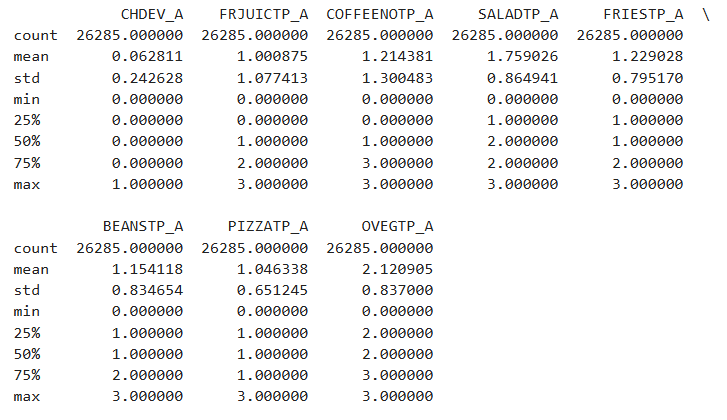
\includegraphics[width=0.6\textwidth]{../Image/P1.jpg}
	\caption{Descriptive Statistics of Life Styles and Coronary Heart Disease}
	\label{fig:P1}
\end{figure}

We can use the correlation matrix to explore the relationship between various variables and show them through visual methods.

\begin{figure}[!h]
	\centering
	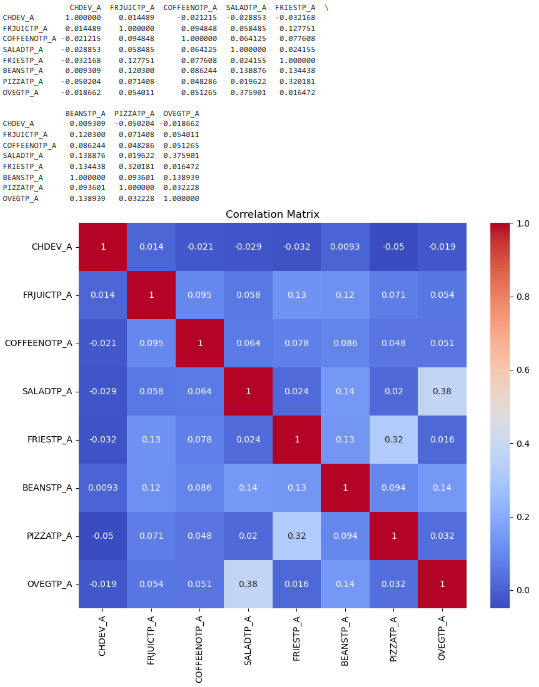
\includegraphics[width=0.5\textwidth]{../Image/P2.jpg}
	\caption{Correlation Matrix of Life Styles and Coronary Heart Disease}
	\label{fig:P2}
\end{figure}

%We'll be able to hypothesis testing to verify two or more statistically significant differences between samples, such as we use in Task2 chi-square, here we use T test to check whether to drink pure fruit juice of Coronary Heart diseases have a significant impact. As shown below, because P < 0.05, the results can be considered statistically significant, the hypothesis can be rejected and a significant difference between the sample means can be considered.

%\begin{figure}[!h]
%	\centering
%	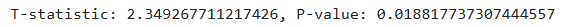
\includegraphics[width=0.7\textwidth]{../Image/P3.jpg}
%	\caption{T test of Life Styles and Coronary Heart Disease}
%	\label{fig:P3}
%\end{figure}

In addition to these kind of statistical methods described above, we can also use some model, to help us better understand and use the data set. According to the figure below, the logistic regression analysis on dietary factors for heart disease showed significant overall model fit (chi2=118.58, p-value=0.0000), with a pseudo R2 of 0.0104. The results indicated that the frequency of fruit juice intake (coefficient=0.0939676, p-value=0.000) and bean intake (coefficient=0.1194858, p-value=0.000) are significantly positively associated with heart disease. Conversely, the frequencies of coffee (coefficient=-0.0507593, p-value=0.015), salad (coefficient=-0.1249328, p-value=0.000), fried potatoes (coefficient=-0.1002222, p-value=0.005), and pizza (coefficient=-0.2981702, p-value=0.000) intake are significantly negatively associated with heart disease. The frequency of other vegetable intake showed no significant association with heart disease (coefficient=-0.0502875, p-value=0.135).

\begin{figure}[!h]
	\centering
	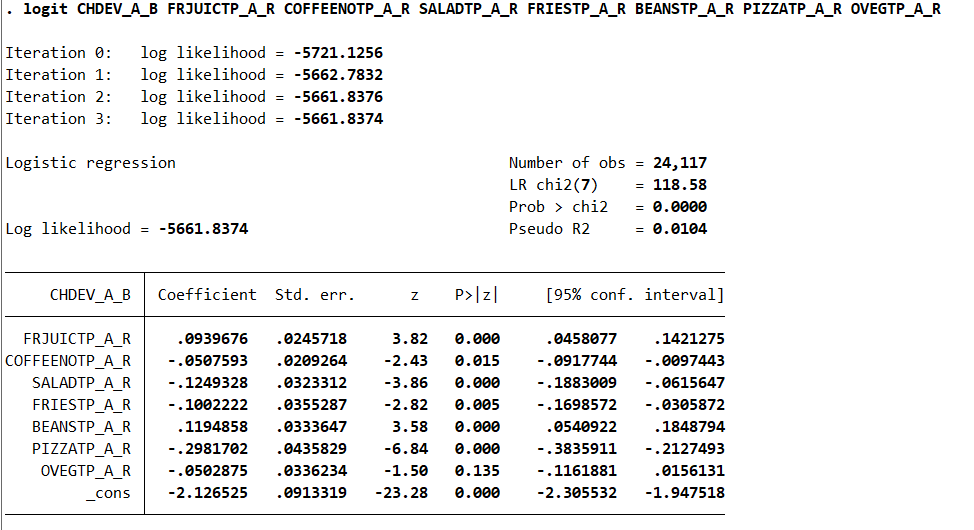
\includegraphics[width=0.8\textwidth]{../Image/L_C.jpg}
	\caption{Life Styles with Coronary Heart Disease}
	\label{fig:G5}
\end{figure}

There are some numerical differences in this result when using different tools, but the general trend is the same. This is probably due to the different processing of the top of the default debit, regularization, optimization of the algorithm and convergence criteria, and so on. graph of the results of doing the same processing in python. When I do the same processing in other diseases, I will release the two images directly.


\begin{figure}[!h]
	\centering
	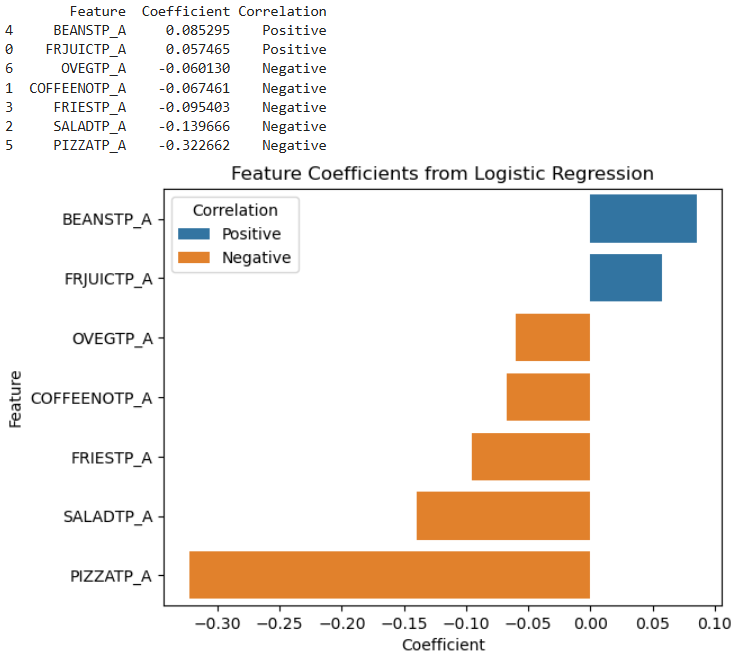
\includegraphics[width=0.5\textwidth]{../Image/P4.png}
	\caption{Feature Coefficients of Life Styles with Coronary Heart Disease}
	\label{fig:P4}
\end{figure}

In addition to logistic regression, we can use other models to make some predictions about pathology diagnosis using data on eating habits. Below I will show how well KNN, K-means, Decision Tree, Random Forest and Catboost models make predictions for Coronary Heart Disease.
\newpage
\begin{figure}[h!]
	\centering
	\begin{minipage}{0.32\textwidth}
		\centering
		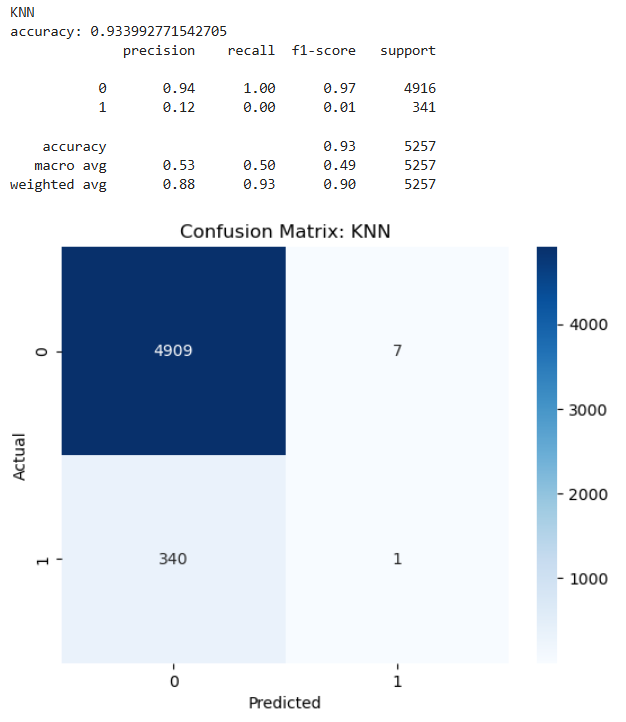
\includegraphics[width=0.9\linewidth]{../Image/P8.jpg}
		\caption{KNN Prediction}
		\label{fig:P8}
	\end{minipage}\hfill
	\begin{minipage}{0.32\textwidth}
		\centering
		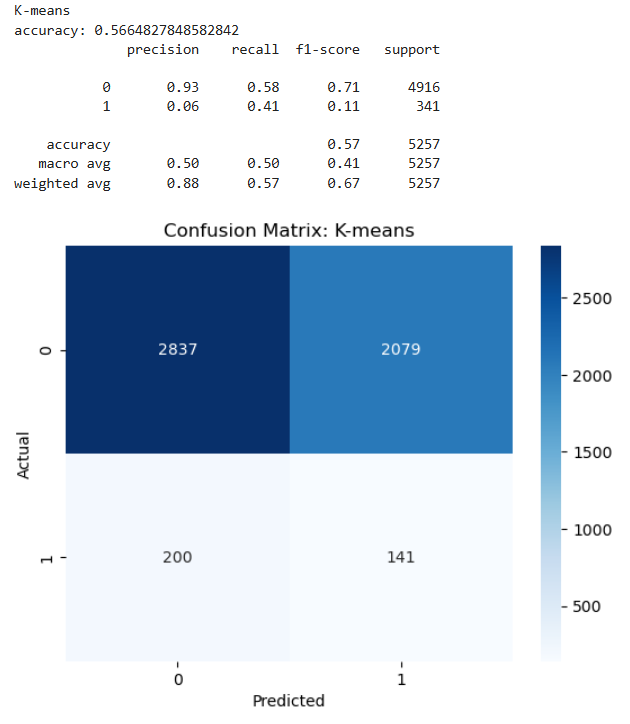
\includegraphics[width=0.9\linewidth]{../Image/P9.jpg}
		\caption{K-means Prediction}
		\label{fig:P9}
	\end{minipage}\hfill
	\begin{minipage}{0.32\textwidth}
		\centering
		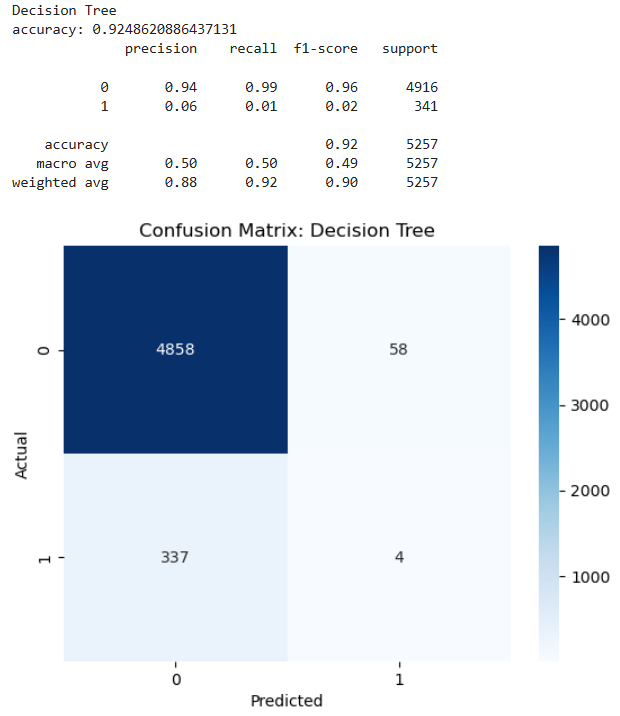
\includegraphics[width=0.9\linewidth]{../Image/P10.jpg}
		\caption{Decision Tree Prediction}
		\label{fig:P10}
	\end{minipage}
	
	\vspace{0.5cm} % Adjust space between rows
	
	\begin{minipage}{0.48\textwidth}
		\centering
		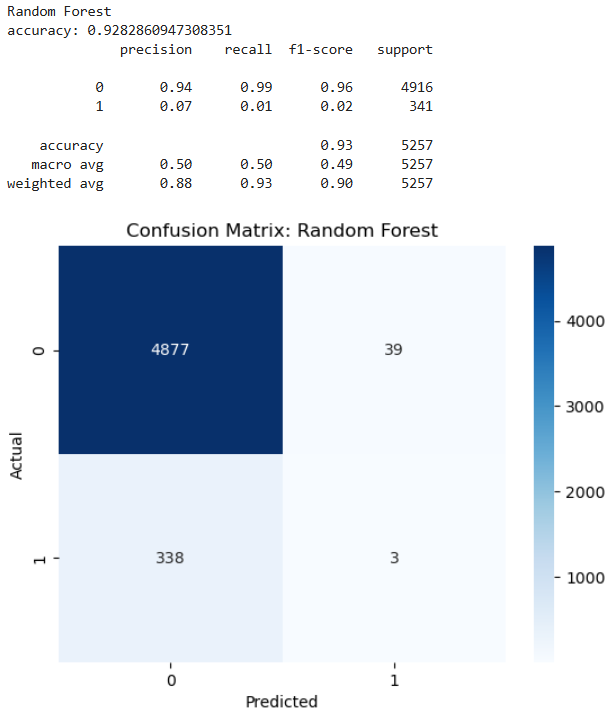
\includegraphics[width=0.7\linewidth]{../Image/P11.jpg}
		\caption{Random Forest Prediction}
		\label{fig:P11}
	\end{minipage}\hfill
	\begin{minipage}{0.48\textwidth}
		\centering
		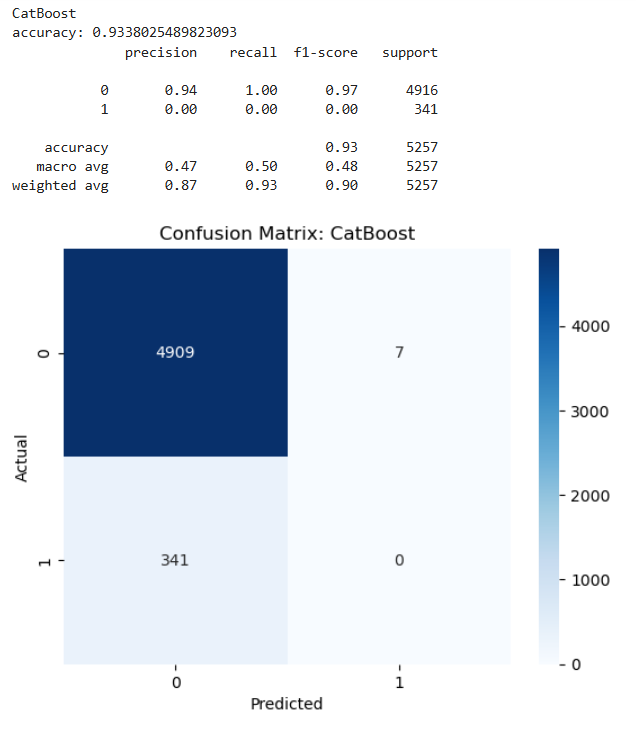
\includegraphics[width=0.7\linewidth]{../Image/P12.jpg}
		\caption{CatBoost Prediction}
		\label{fig:P12}
	\end{minipage}
	%\caption{Overall caption for the figure}
	%\label{fig:all_pictures}
\end{figure}

From the above five images, it can be noticed that KNN, Random Forest and Catboost have the best prediction performance. K-means performs worse because it is a clustering algorithm, not a classification algorithm. Its goal is to categorize the data into K clusters, not to predict category labels, and K-means is very sensitive to noise. I will not show the K-means results when dealing with other cardiovascular diseases.

In addition, the Decision Tree, the Random Forest and Catboost because of their model features, we can observe it features of reference importance, as shown in the figure below.

\begin{figure}[h!]
	\centering
	\begin{minipage}{0.32\textwidth}
		\centering
		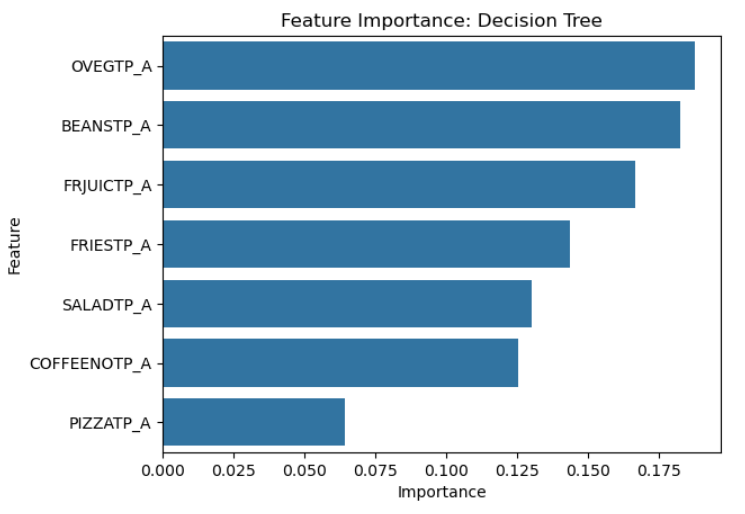
\includegraphics[width=0.9\linewidth]{../Image/P13.jpg}
		\caption{Decision Tree Feature Importance}
		\label{fig:P13}
	\end{minipage}\hfill
	\begin{minipage}{0.32\textwidth}
		\centering
		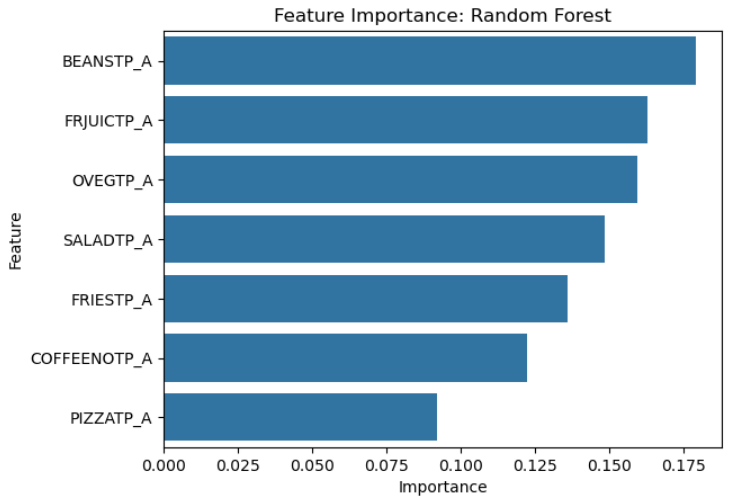
\includegraphics[width=0.9\linewidth]{../Image/P14.jpg}
		\caption{Random Forest Feature Importance}
		\label{fig:P14}
	\end{minipage}\hfill
	\begin{minipage}{0.32\textwidth}
		\centering
		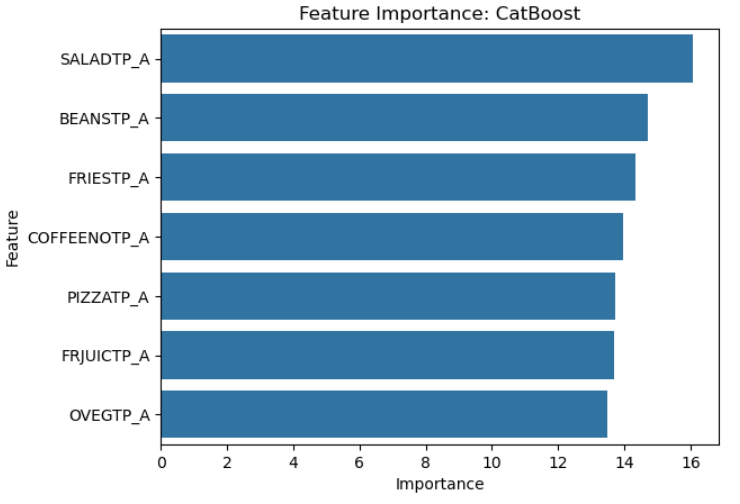
\includegraphics[width=0.9\linewidth]{../Image/P15.jpg}
		\caption{CatBoost Importance}
		\label{fig:P15}
	\end{minipage}
\end{figure}

\subsubsection{Life Styles with Angina}

In explore the life styles and the relationship between Angina, we can also finish a Correlation Matrix, to roughly understand the relations between the coefficient of each variable.

\begin{figure}[!h]
	\centering
	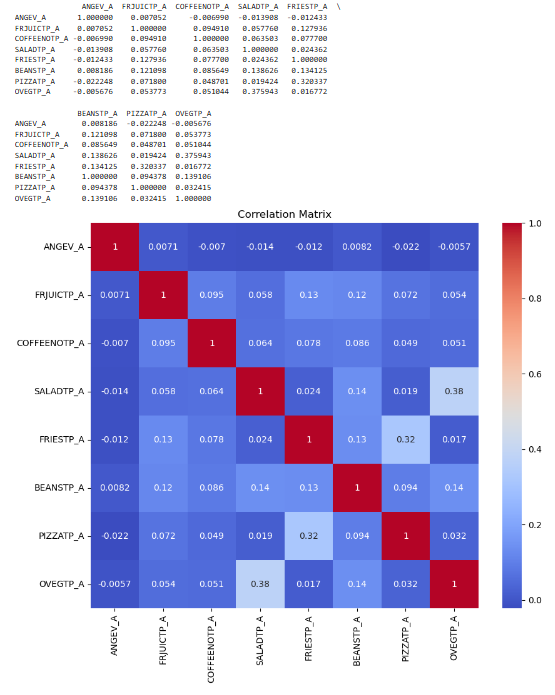
\includegraphics[width=0.5\textwidth]{../Image/P5.jpg}
	\caption{Correlation Matrix of Life Styles and Angina}
	\label{fig:P5}
\end{figure}

%Similarly we can use the T test to determine whether the variable is significant with angina or not. The graph below shows P > 0.05, which meets the original hypothesis, indicating that there is no statistically significant relationship between whether or not drinking pure fruit juice to drink is diagnosed with angina.
%\newpage
%\begin{figure}[!h]
%	\centering
%	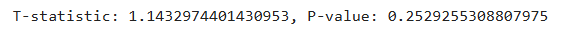
\includegraphics[width=0.7\textwidth]{../Image/P6.jpg}
%	\caption{T test of Life Styles and Angina}
%	\label{fig:P6}
%\end{figure}

By investigating the association of dietary habits with Angina by logistic regression, we obtained the following figure. By this figure we can find that drink pure fruit juice, drink coffee with sugar, eat salad, fired potatoes and other vegetables while all showed a certain negative correlation, but they all crossed zero at the 95\% confidence interval value, it makes them in the statistical significance is not big, low influence not for reference. While eating beans was significantly positive correlation in the survey, using the pizza for significant negative correlation.

\begin{figure}[!h]
	\centering
	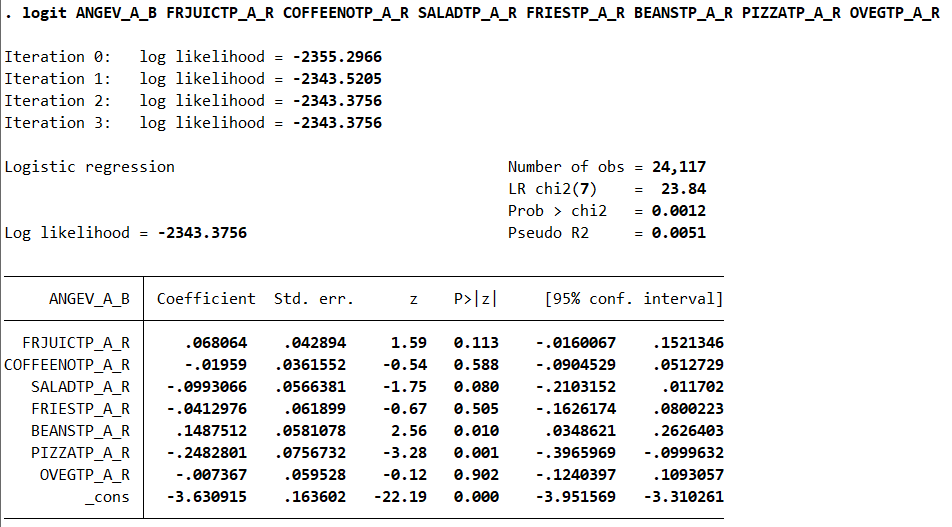
\includegraphics[width=0.8\textwidth]{../Image/L_A.jpg}
	\caption{Life Styles with Angina}
	\label{fig:G6}
\end{figure}

\begin{figure}[!h]
	\centering
	\includegraphics[width=0.6\textwidth]{../Image/P7.jpg}
	\caption{Feature Coefficients of Life Styles with Angina}
	\label{fig:P7}
\end{figure}

Four models, KNN, Decision Tree, Random Forest and CatBoost are used to predict the probability that Angina is diagnosed. And the associated feature importance picture is obtained as shown below.

\begin{figure}[h!]
	\begin{minipage}{0.48\textwidth}
		\centering
		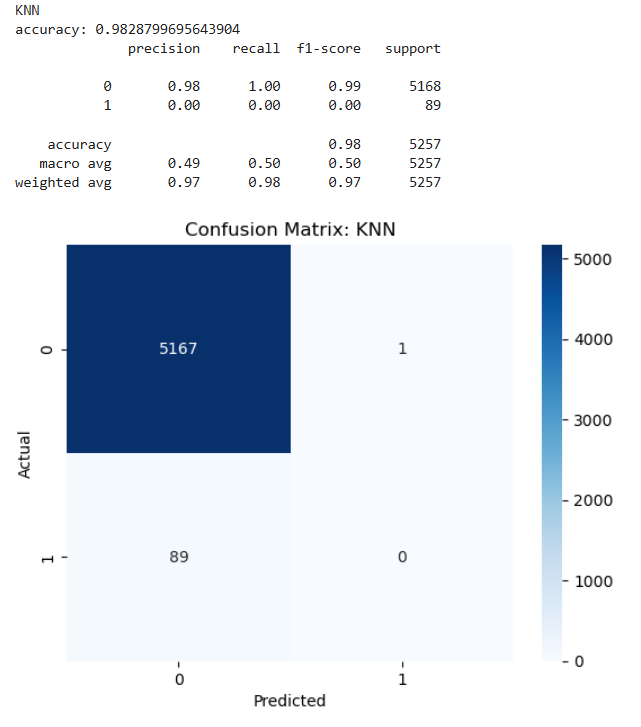
\includegraphics[width=0.6\linewidth]{../Image/P16.jpg}
		\caption{KNN Prediction}
		\label{fig:P16}
	\end{minipage}\hfill
	\begin{minipage}{0.48\textwidth}
		\centering
		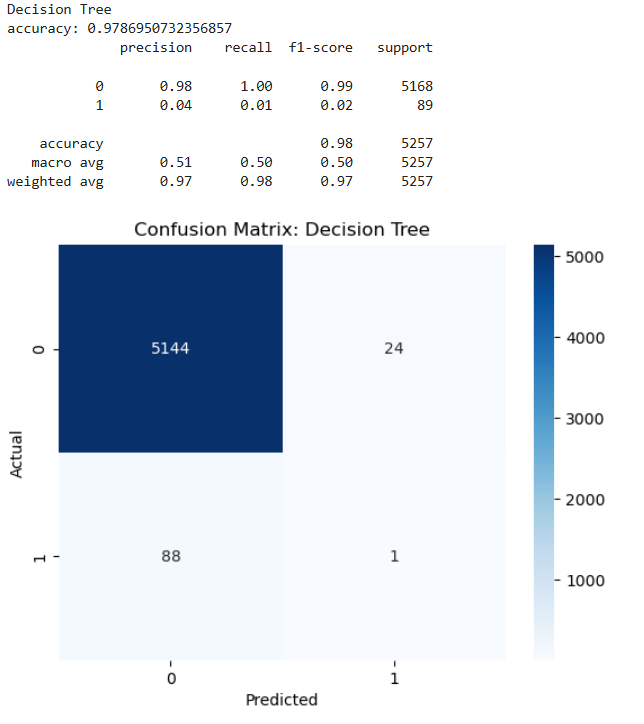
\includegraphics[width=0.6\linewidth]{../Image/P17.jpg}
		\caption{Decision Tree Prediction}
		\label{fig:P17}
	\end{minipage}
	
	\vspace{0.5cm} % Adjust space between rows
	
	\begin{minipage}{0.48\textwidth}
		\centering
		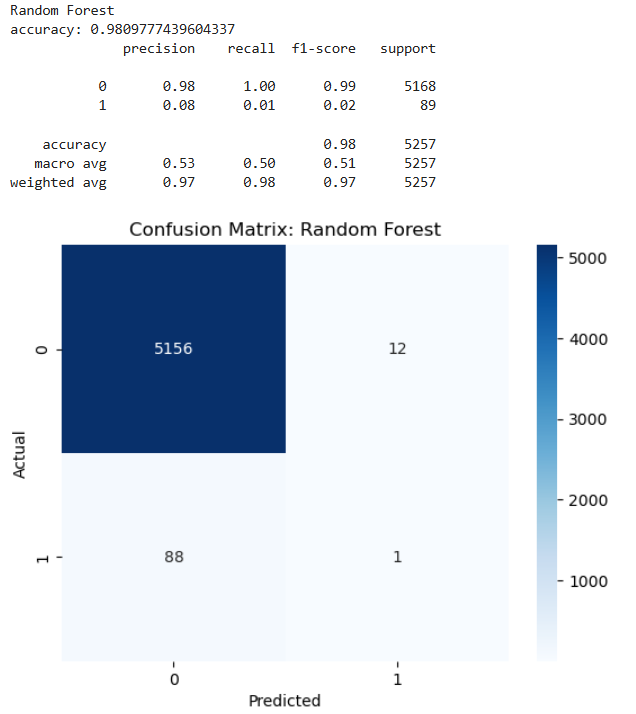
\includegraphics[width=0.6\linewidth]{../Image/P18.jpg}
		\caption{Random Forest Prediction}
		\label{fig:P18}
	\end{minipage}\hfill
	\begin{minipage}{0.48\textwidth}
		\centering
		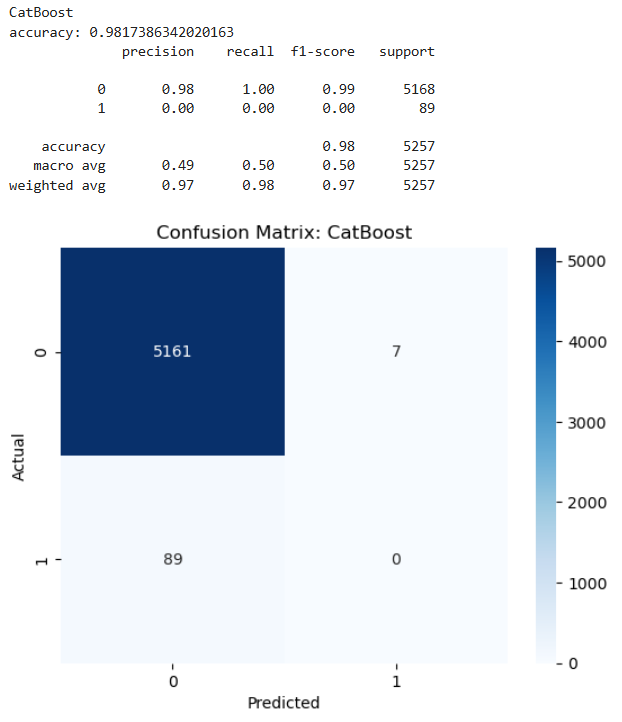
\includegraphics[width=0.6\linewidth]{../Image/P19.jpg}
		\caption{CatBoost Prediction}
		\label{fig:P19}
	\end{minipage}
\end{figure}

\begin{figure}[h!]
	\centering
	\begin{minipage}{0.32\textwidth}
		\centering
		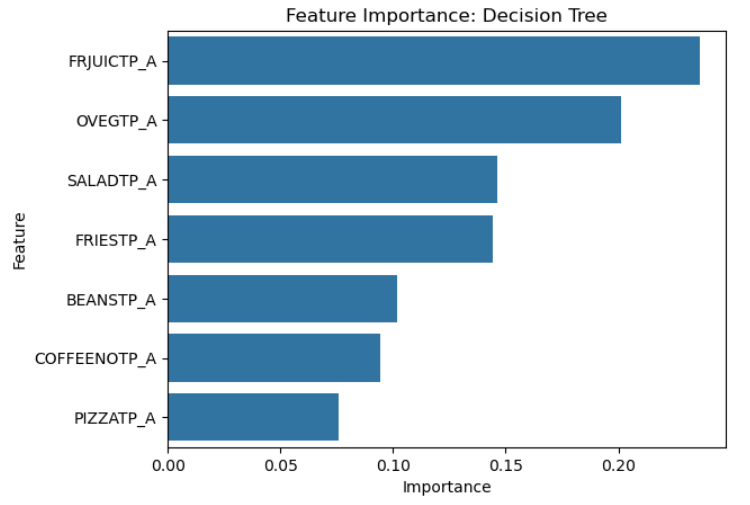
\includegraphics[width=0.9\linewidth]{../Image/P20.jpg}
		\caption{Decision Tree Feature Importance}
		\label{fig:P20}
	\end{minipage}\hfill
	\begin{minipage}{0.32\textwidth}
		\centering
		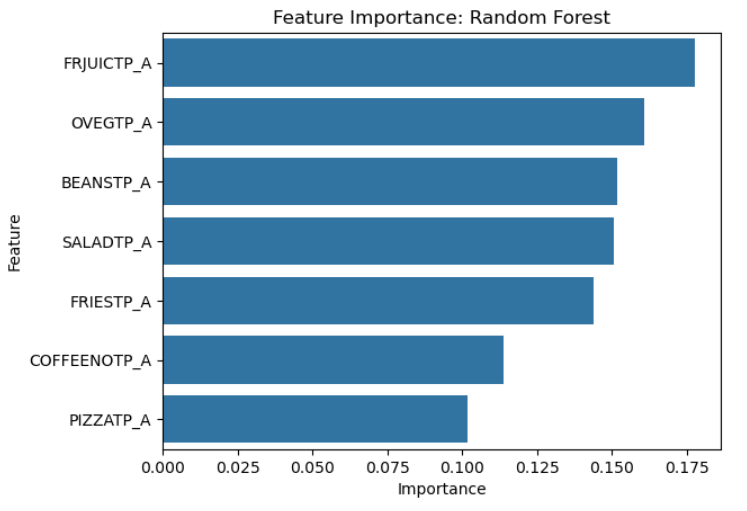
\includegraphics[width=0.9\linewidth]{../Image/P21.jpg}
		\caption{Random Forest Feature Importance}
		\label{fig:P21}
	\end{minipage}\hfill
	\begin{minipage}{0.32\textwidth}
		\centering
		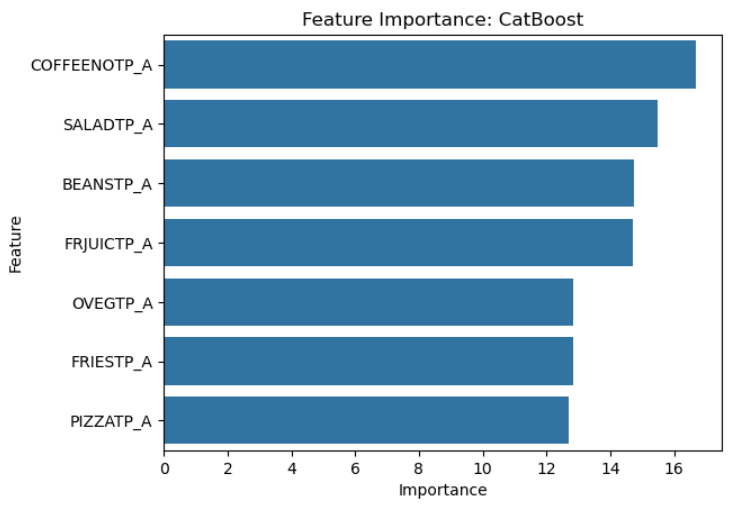
\includegraphics[width=0.9\linewidth]{../Image/P22.jpg}
		\caption{CatBoost Importance}
		\label{fig:P22}
	\end{minipage}
\end{figure}

\subsubsection{Life Styles with Heart Attack}

When dealing with Life Styles and Heart Attack, we still first look at their correlation matrix to get a general idea of the coefficient relationship between these variables, and also to get a general idea of the importance of the variables.

\begin{figure}[!h]
	\centering
	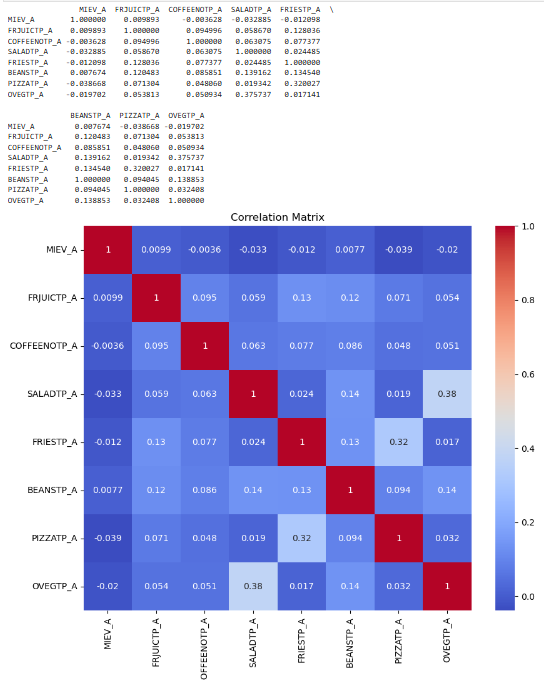
\includegraphics[width=0.5\textwidth]{../Image/P23.jpg}
	\caption{Correlation Matrix of Life Styles and Heart Attack}
	\label{fig:P5}
\end{figure}

%In this case, we performed a T test to notice that the hypothesis of the T test was violated due to P > 0.05,which indicates that the relationship between Heart Attack and drinking pure fruit juice is not statistically significant.

%\begin{figure}[!h]
%	\centering
%	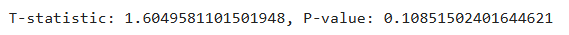
\includegraphics[width=0.7\textwidth]{../Image/P25.jpg}
%	\caption{T test of Life Styles and Heart Attack}
%	\label{fig:P25}
%\end{figure}

Investigating the association between dietary habits and Heart Attack through logistic regression, we obtained the following graph. From this figure we can find that drinking sweetened coffee and eating fired potatoes still both cross the 0 value within the 95\% confidence interval and their p-values are greater than 0.5, indicating that their effects are not significant. While quoting pure fruit juice and using beans are significantly positively correlated in this survey. The use of salads and pizzas were significantly negatively correlated.
\newpage
\begin{figure}[!h]
	\centering
	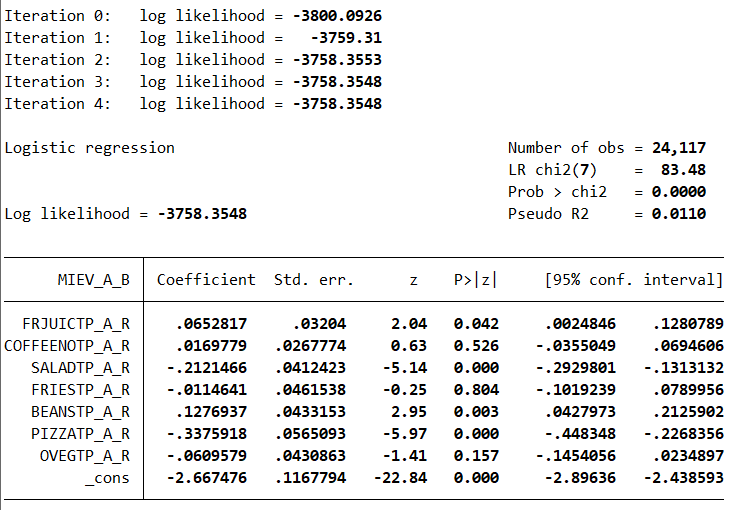
\includegraphics[width=0.7\textwidth]{../Image/L_M.jpg}
	\caption{Life Styles with Heart Attack}
	\label{fig:G7}
\end{figure}

\begin{figure}[!h]
	\centering
	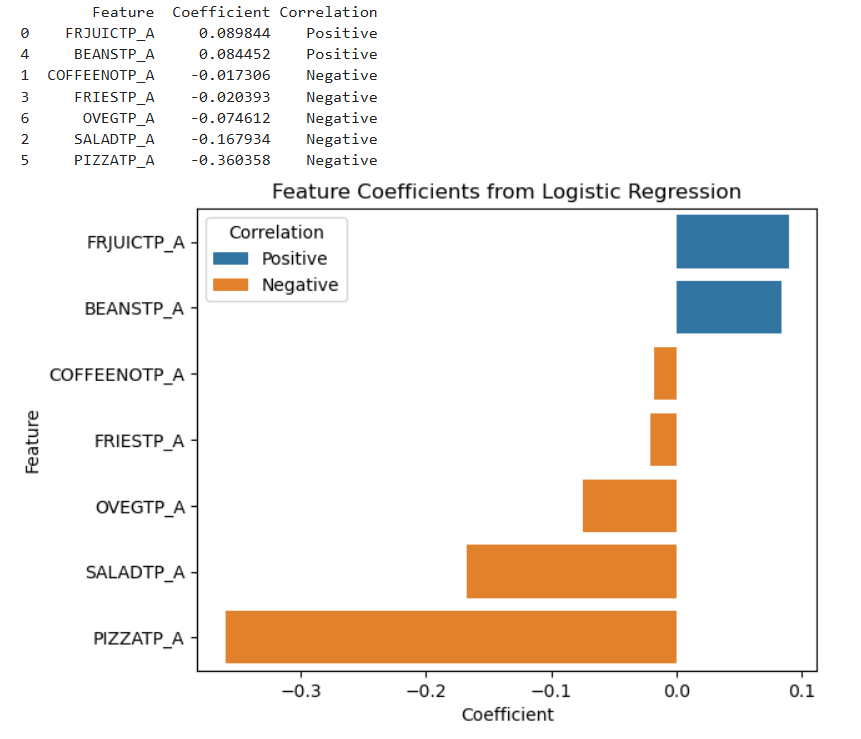
\includegraphics[width=0.6\textwidth]{../Image/P24.jpg}
	\caption{Feature Coefficients of Life Styles with Heart Attack}
	\label{fig:P24}
\end{figure}

We also make a prediction of Heart Attack being diagnosed using the four models described above, and their predictions are shown below.

\newpage
\begin{figure}[h!]
	\begin{minipage}{0.48\textwidth}
		\centering
		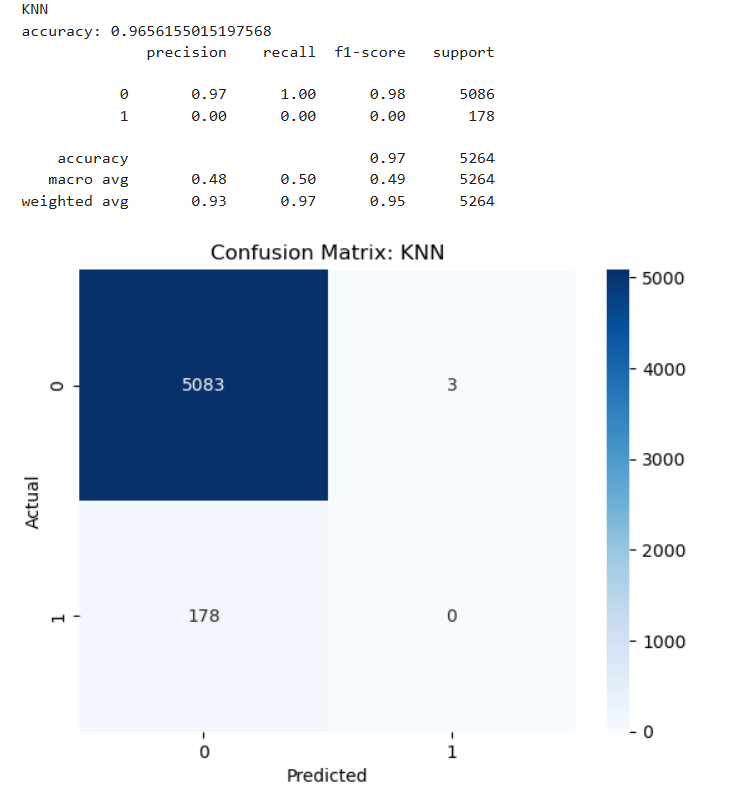
\includegraphics[width=0.7\linewidth]{../Image/P26.jpg}
		\caption{KNN Prediction}
		\label{fig:P26}
	\end{minipage}\hfill
	\begin{minipage}{0.48\textwidth}
		\centering
		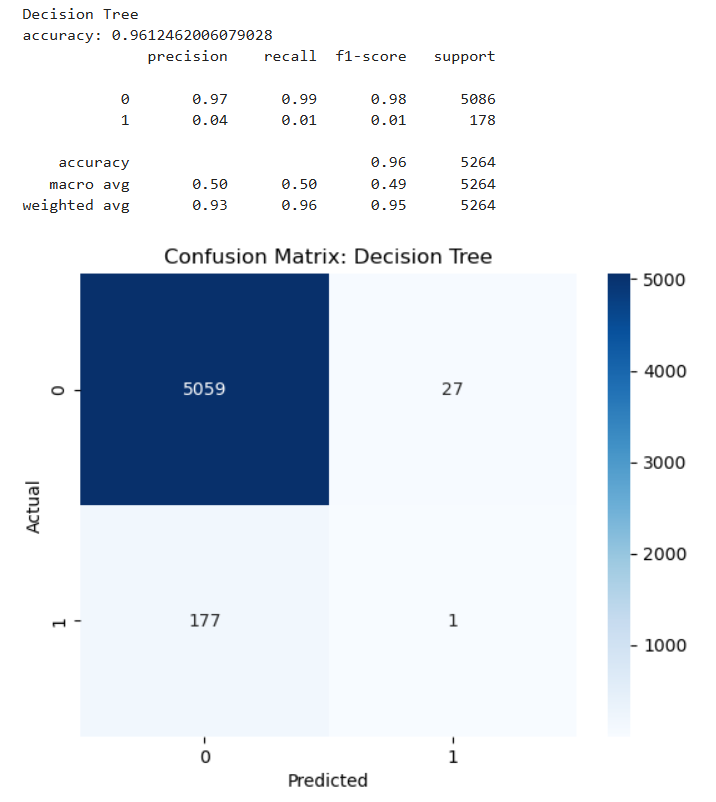
\includegraphics[width=0.7\linewidth]{../Image/P28.jpg}
		\caption{Decision Tree Prediction}
		\label{fig:P28}
	\end{minipage}
	
	\vspace{0.5cm} % Adjust space between rows
	
	\begin{minipage}{0.48\textwidth}
		\centering
		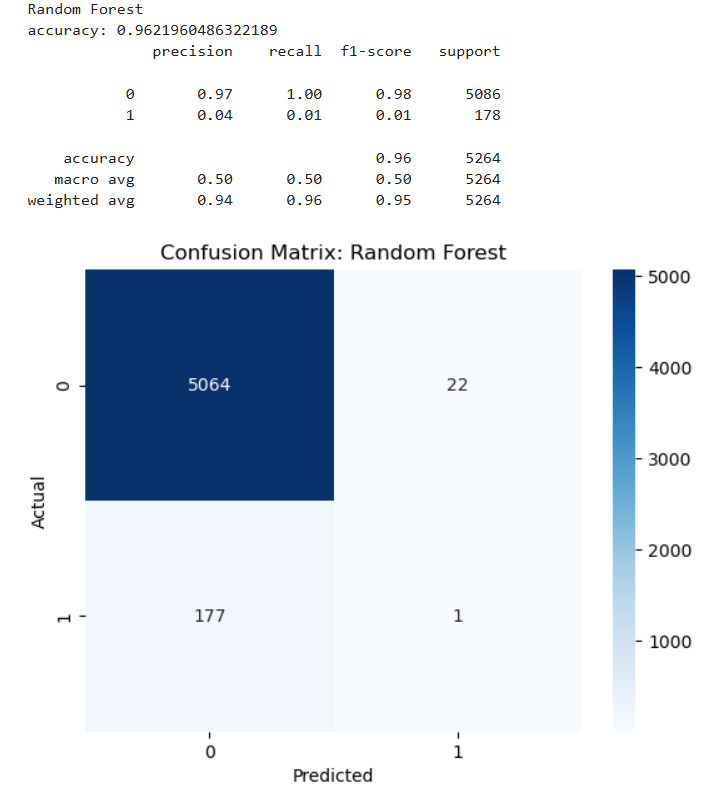
\includegraphics[width=0.7\linewidth]{../Image/P29.jpg}
		\caption{Random Forest Prediction}
		\label{fig:P29}
	\end{minipage}\hfill
	\begin{minipage}{0.48\textwidth}
		\centering
		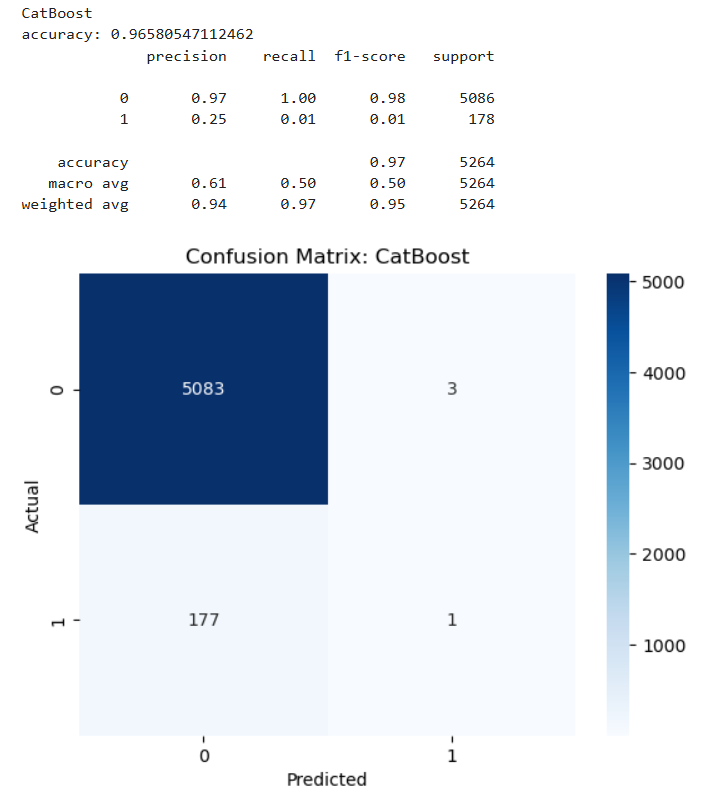
\includegraphics[width=0.7\linewidth]{../Image/P30.jpg}
		\caption{CatBoost Prediction}
		\label{fig:P30}
	\end{minipage}
\end{figure}

\begin{figure}[h!]
	\centering
	\begin{minipage}{0.32\textwidth}
		\centering
		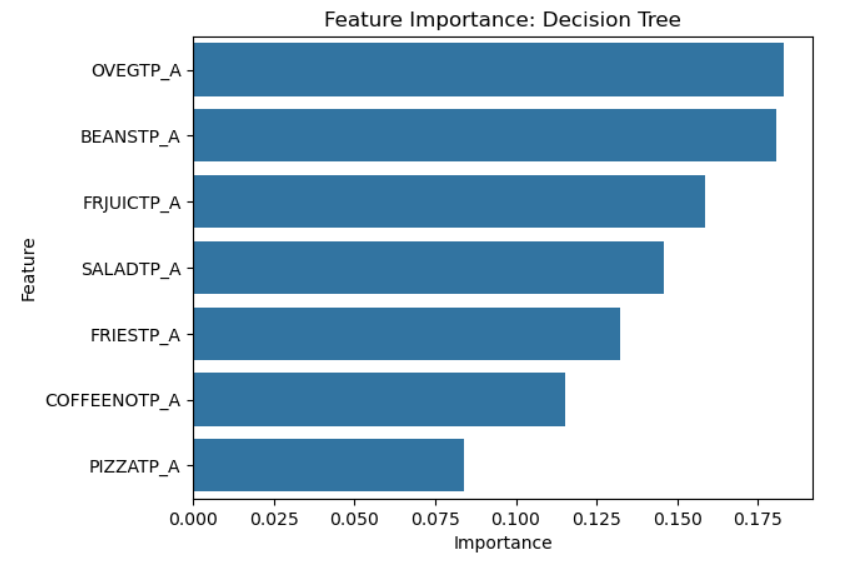
\includegraphics[width=0.9\linewidth]{../Image/P31.jpg}
		\caption{Decision Tree Feature Importance}
		\label{fig:P31}
	\end{minipage}\hfill
	\begin{minipage}{0.32\textwidth}
		\centering
		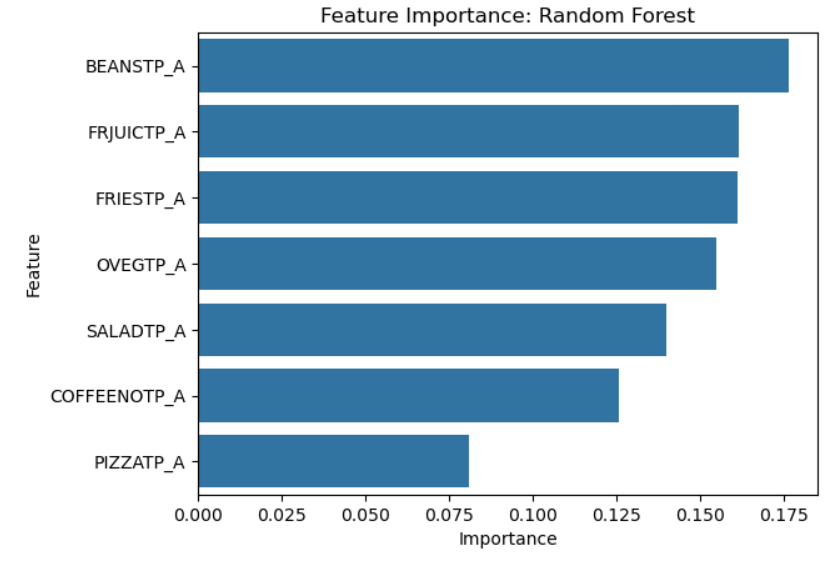
\includegraphics[width=0.9\linewidth]{../Image/P32.jpg}
		\caption{Random Forest Feature Importance}
		\label{fig:P32}
	\end{minipage}\hfill
	\begin{minipage}{0.32\textwidth}
		\centering
		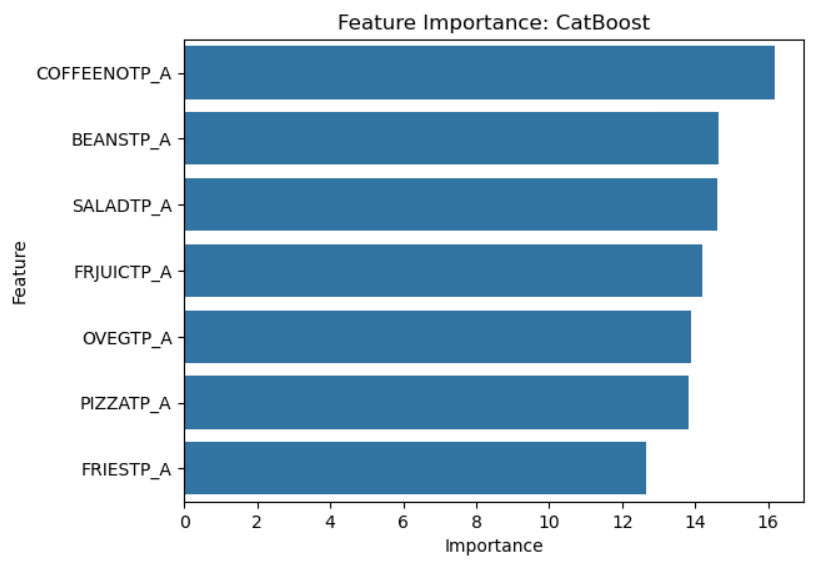
\includegraphics[width=0.9\linewidth]{../Image/P33.jpg}
		\caption{CatBoost Importance}
		\label{fig:P33}
	\end{minipage}
\end{figure}



\subsubsection{Life Styles with Stroke}

The following figure shows the coefficient relationship between various dietary habits and stroke in the dataset.
\newpage
\begin{figure}[!h]
	\centering
	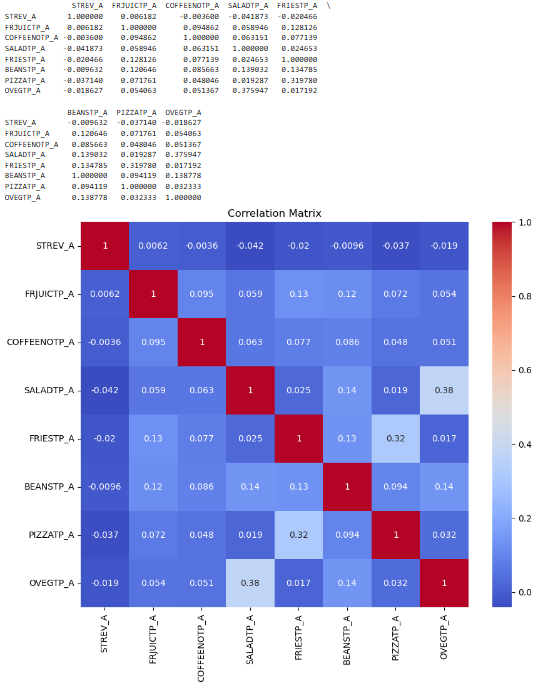
\includegraphics[width=0.5\textwidth]{../Image/P34.jpg}
	\caption{Correlation Matrix of Life Styles and Stroke}
	\label{fig:P34}
\end{figure}

%In this case, we noticed that the hypothesis of the T test was violated due to P > 0.05, which indicates that the relationship between Stroke and drinking pure fruit juice is not statistically significant.

%\begin{figure}[!h]
%	\centering
%	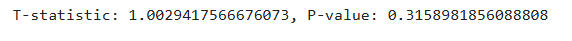
\includegraphics[width=0.7\textwidth]{../Image/P35.jpg}
%	\caption{T test of Life Styles and Stroke}
%	\label{fig:P35}
%\end{figure}



Analyzing the relationship between dietary habits and stroke through logistic regression, we obtained the following results: as can be seen from the graph, sweetened coffee, fried potatoes, beans, or other vegetables all crossed a value of 0 or had a p-value of greater than 0.5 within the 95\% confidence interval, suggesting that they did not have a significant effect. However, pure fruit juices showed a significant positive correlation in the survey, while salads and pizzas showed a significant negative correlation.

\begin{figure}[!h]
	\centering
	\includegraphics[width=0.7\textwidth]{../Image/L_S.jpg}
	\caption{Life Styles with Stroke}
	\label{fig:G8}
\end{figure}
\newpage
\begin{figure}[!h]
	\centering
	\includegraphics[width=0.6\textwidth]{../Image/P36.jpg}
	\caption{Feature Coefficients of Life Styles with Stroke}
	\label{fig:P36}
\end{figure}

The next images will show how well the four models predict stroke, and the importance of the variables in these models.

\begin{figure}[h!]
	\begin{minipage}{0.48\textwidth}
		\centering
		\includegraphics[width=0.6\linewidth]{../Image/P37.jpg}
		\caption{KNN Prediction}
		\label{fig:P37}
	\end{minipage}\hfill
	\begin{minipage}{0.48\textwidth}
		\centering
		\includegraphics[width=0.6\linewidth]{../Image/P38.jpg}
		\caption{Decision Tree Prediction}
		\label{fig:P38}
	\end{minipage}
	
	\vspace{0.5cm} % Adjust space between rows
	
	\begin{minipage}{0.48\textwidth}
		\centering
		\includegraphics[width=0.6\linewidth]{../Image/P39.jpg}
		\caption{Random Forest Prediction}
		\label{fig:P39}
	\end{minipage}\hfill
	\begin{minipage}{0.48\textwidth}
		\centering
		\includegraphics[width=0.6\linewidth]{../Image/P40.jpg}
		\caption{CatBoost Prediction}
		\label{fig:P40}
	\end{minipage}
\end{figure}
\newpage
\begin{figure}[h!]
	\centering
	\begin{minipage}{0.32\textwidth}
		\centering
		\includegraphics[width=0.9\linewidth]{../Image/P41.jpg}
		\caption{Decision Tree Feature Importance}
		\label{fig:P41}
	\end{minipage}\hfill
	\begin{minipage}{0.32\textwidth}
		\centering
		\includegraphics[width=0.9\linewidth]{../Image/P42.jpg}
		\caption{Random Forest Feature Importance}
		\label{fig:P42}
	\end{minipage}\hfill
	\begin{minipage}{0.32\textwidth}
		\centering
		\includegraphics[width=0.9\linewidth]{../Image/P43.jpg}
		\caption{CatBoost Importance}
		\label{fig:P43}
	\end{minipage}
\end{figure}

\subsubsection{Evaluation}

The conclusions generated by these statistical software programs cannot be used to develop a dietary program and may even be contrary to your doctor's recommendations. These preliminary conclusions are based on statistical calculations only and are therefore influenced by the data set used. In performing the logistic regression analysis, although I cleaned the data and selected the variables, the results may be subject to error due to factors such as modeling and sample representativeness. The variables selected may not be representative enough or selected in a limited direction, and some variables may need to work together to show a certain effect. Each conclusion can only reflect the statistically specific performance of the data set used.

For model prediction accuracy, we take the KNN model for Coronary Heart Disease as an example. Although the prediction accuracy of this model is as high as 93\%, if we look at the other parameters in detail, we can see that the model performs very poorly for category 1 (diagnosis of Coronary Heart Disease). The model almost completely ignores category 1, recognizing only 1 of the 341 category 1s in the test, and incorrectly identifying 7 category 0s as category 1s, resulting in false-positive cases. This resulted in low precision, recall and F1-score for category 1. This problem is usually caused by an imbalance in the number of categories. In the future, we can adjust the categorie weights so that the model focuses more on a small number of classes. Or train a better model by hyperparameterization.


\subsection{Life Styles with BMI}

The figure below shows the coefficient relationship between various dietary habits and BMI in the data set. 

\begin{figure}[!h]
	\centering
	\includegraphics[width=0.3\textwidth]{../Image/P44.jpg}
	\caption{Correlation Matrix of Life Styles and BMI}
	\label{fig:P44}
\end{figure}

%We can also confirm from the side by T test that most of the parameters have no statistically %significant effect on BMI.

%\begin{figure}[!h]
%	\centering
%	\includegraphics[width=0.7\textwidth]{../Image/P45.jpg}
%	\caption{T test of Life Styles and BMI}
%	\label{fig:P45}
%\end{figure}

In the above we are proceeding with logistic regression using stata, simply because the dependent variable of logistic regression is binary. And below we are going to explore the relationship between BMI and life styles, in our codebook, BMI is categorized into four degrees, so logistic regression is no longer applicable. Here we consider Ordered Logistic Regression or Multinomial Logistic Regression. and because BMI as the dependent variable, 1, 2, 3, 4 indicates four different degrees, we choose to use Ordered Logistic Regression.

As shown in the figure below, drinking pure fruit juice, eating salads with sugar coffee or tee, beans and other vegetables are all significantly negatively correlated with BMI. While eating fried potatoes and pizza had a significant positive correlation with BMI. It should be noted that none of the food items with positive or negative correlations were better with more. Maintaining a healthy BMI requires eating the right diet.

\begin{figure}[!h]
	\centering
	\includegraphics[width=0.8\textwidth]{../Image/OL_BMI.jpg}
	\caption{Life Styles with BMI}
	\label{fig:G9}
\end{figure}

\begin{figure}[!h]
	\centering
	\includegraphics[width=0.6\textwidth]{../Image/P46.jpg}
	\caption{Feature Coefficients of Life Styles with BMI}
	\label{fig:P46}
\end{figure}

When dealing with the relationship between life styles and BMI, I still used the previous four models to make predictions. Here are the models of rendering and variable importance.

\newpage
\begin{figure}[h!]
	\begin{minipage}{0.48\textwidth}
		\centering
		\includegraphics[width=0.7\linewidth]{../Image/P47.jpg}
		\caption{KNN Prediction}
		\label{fig:P47}
	\end{minipage}\hfill
	\begin{minipage}{0.48\textwidth}
		\centering
		\includegraphics[width=0.7\linewidth]{../Image/P48.jpg}
		\caption{Decision Tree Prediction}
		\label{fig:P48}
	\end{minipage}
	
	\vspace{0.5cm} % Adjust space between rows
	
	\begin{minipage}{0.48\textwidth}
		\centering
		\includegraphics[width=0.7\linewidth]{../Image/P49.jpg}
		\caption{Random Forest Prediction}
		\label{fig:P49}
	\end{minipage}\hfill
	\begin{minipage}{0.48\textwidth}
		\centering
		\includegraphics[width=0.7\linewidth]{../Image/P50.jpg}
		\caption{CatBoost Prediction}
		\label{fig:P50}
	\end{minipage}
\end{figure}
\begin{figure}[h!]
	\centering
	\begin{minipage}{0.32\textwidth}
		\centering
		\includegraphics[width=0.9\linewidth]{../Image/P51.jpg}
		\caption{Decision Tree Feature Importance}
		\label{fig:P51}
	\end{minipage}\hfill
	\begin{minipage}{0.32\textwidth}
		\centering
		\includegraphics[width=0.9\linewidth]{../Image/P52.jpg}
		\caption{Random Forest Feature Importance}
		\label{fig:P52}
	\end{minipage}\hfill
	\begin{minipage}{0.32\textwidth}
		\centering
		\includegraphics[width=0.9\linewidth]{../Image/P53.jpg}
		\caption{CatBoost Importance}
		\label{fig:P53}
	\end{minipage}
\end{figure}

\subsubsection{Evaluation}

We can find that the model does not perform well in predicting BMI. A big reason for this is that our code uses the most basic parameters and does not spend enough time on feature engineering and hyperparameter model training. Moreover, the dataset itself is not uniformly distributed across BMI categories, which also has a certain impact on the training of classification algorithms. If the future have more time for training, we can get a good accuracy of BMI prediction model.

\newpage
\section{Task 4}

In this section, I will explain to you the mathematical analysis software used in this report. I analyzed the data in this report using Stata. Stata is a powerful statistical analysis software that is widely used in various research fields. For this report, Stata was selected because of its flexible data processing capabilities and rich statistical analysis capabilities, as well as its processing advantages over complex data sets. In addition, its powerful graphing capabilities help me visually describe the relationships between various variables and the trends of disease as they change. It can also export forms directly into latex format, helping me fill out the results in my report accurately and completely.

During the completion of the report, I wrote all the do scripts in the attachments folder. They all end up producing an image or table for this report. Before writing each do file script, I clarify its purpose: what I need this do file to accomplish and which data and variables it will utilize. Then, I preprocess the data and variables that will be used. The main task of preprocessing is to clean out invalid or potentially influential data that could affect subsequent results. While reviewing the codebook and dataset, I noticed that most codes provided options such as "unknown," "uncertain," or "refused" for respondents. Such data was not helpful to our research and might have an impact on our data processing. Once, I forgot to exclude them, resulting in several extra bars in a bar chart where there should have been only two. Therefore, during preprocessing, it's crucial to remove such data. This step ensures data quality and consistency, laying the groundwork for subsequent analysis.

In terms of defining and selecting variables, we comprehensively chose the four cardiovascular-related diseases outlined in the codebook to conduct a more thorough analysis. Additionally, for demographic variables, we selected fundamental and widely applicable ones such as age, sex, race, address, and housing type. Regarding lifestyle aspects, in Task 2, we primarily focused on dietary habits because the codebook provided detailed dietary-related data. These types of data also correlate well with demographic variables. In Task 3, we conducted a more detailed study on lifestyle aspects, further exploring the relationships between dietary habits, body mass index, and cardiovascular diseases. Thanks to the tables provided by Stata, we were able to clearly describe the probability of disease occurrence under multiple factors.

In terms of statistical methods, I used the chi-square test, logistic regression analysis, ordered logistic regression, comparative bar graphs, multiway tables, and many other useful graphical tools that stata offers. This is one of the main reasons why I chose stata as a data analysis tool, it provides statistical tools that can be extremely easy to use, such as the chi-square test, which stata encapsulates into a function that requires only a few words to use, which provides me with great convenience. The selection and application of these statistical methods can help to gain a deeper understanding of the impact of lifestyle factors on cardiovascular health and provide a scientific basis and guidance for future prevention strategies and clinical management.

In order to explore whether the variables are significantly correlated with each other, I also considered using the T test method at the very beginning. However, the T test will perform much better with normally distributed continuous variables, and performs mediocre with our discrete categorical data. So I used the chi-square test which is more suitable for our dataset to confirm whether the variables are significantly correlated with each other. In fact, in this report, I am constantly trying to determine the significant correlation between variables, both qualitatively and quantitatively. I used stata's chi-square test. Results from logistic regression or ordinal logistic regression were used to see values within 95\% confidence intervals. I trained multiple models using python to demonstrate correlation between variables by looking at feature importance. I also use correlation coefficients between variables to illustrate the degree of correlation between variables and outcomes.

In addition to using Stata for data processing and statistical analysis, I carried out further work using Python, a flexible and powerful programming language that not only excels in data cleaning and preprocessing, but also demonstrates its power in building and evaluating machine learning models. I also tried to use the dataset and the model to make predictions about disease conditions and BMI conditions. In these areas, python excelled, and its flexibility and ease of writing and modifying allowed me to get a lot of models and experimental data. As I introduced in the Task3, I use the four machine learning algorithms and models. With more time in the future, I can get better models with more practical significance through a lot of cross-validation and hyper-parameter tuning.


I also use Jupyter Notebook, which, with its interactivity, instant feedback, and powerful visualization capabilities, allows me to see the results of my data visualizations clearly and intuitively as I run the Python code, making the process of analyzing the data much more concise and easy to understand.


\newpage
\section{Task 5}
All scripts, images, etc. will be submitted as attachments. Please note that I am using Stata MP 17, if you need to test my scripts, please use the same version number in case some modules may not work. Also all do files need to be run in the same folder as “adult22.csv” or you may need to go into the do file and change the path. 

When testing the correlation between lifestyle habits and CVC in Task3, there were some conclusions I wondered if I was doing it wrong. I ran a logistic regression in python to test this as well. The results are shown in the figure below, and it can be seen that although the correlation values are different, the overall trend of positive and negative correlation is not wrong. The different values may be due to different processing of the top of the default debit, regularization, optimization of the algorithm and convergence criteria, and so on. But it confirms that my general direction is correct. The code can be found in the folder “python\_version”.

\begin{figure}[!h]
	\centering
	\includegraphics[width=0.8\textwidth]{../Image/python.jpg}
	\caption{Python Result}
	\label{fig:G10}
\end{figure}

In addition, all the machine learning related code is in the "python\_version folder". These ipynb files should be run through jupyter notebook.

\end{document}
